\documentclass[10pt,a4paper,titlepage,openany,oneside]{memoir}

%% `usepackage` commands.
%% Packages
%% ========
\usepackage{wrapfig}

%% LaTeX Font encoding -- DO NOT CHANGE
\usepackage[OT1]{fontenc}

%% Babel provides support for languages.  'english' uses British
%% English hyphenation and text snippets like "Figure" and
%% "Theorem". Use the option 'ngerman' if your document is in German.
%% Use 'american' for American English.  Note that if you change this,
%% the next LaTeX run may show spurious errors.  Simply run it again.
%% If they persist, remove the .aux file and try again.
\usepackage[english]{babel}

%% Input encoding 'utf8'. In some cases you might need 'utf8x' for
%% extra symbols. Not all editors, especially on Windows, are UTF-8
%% capable, so you may want to use 'latin1' instead.
\usepackage[utf8]{inputenc}

%% This changes default fonts for both text and math mode to use Herman Zapfs
%% excellent Palatino font. Do not change this.
\usepackage[sc]{mathpazo}

%% The AMS-LaTeX extensions for mathematical typesetting.  Do not
%% remove.
\usepackage{amsmath,amssymb,amsfonts,mathrsfs}
\allowdisplaybreaks

%% NTheorem is a reimplementation of the AMS Theorem package. This
%% will allow us to typeset theorems like examples, proofs and
%% similar.  Do not remove.
%% NOTE: Must be loaded AFTER amsmath, or the \qed placement will
%% break
\usepackage[amsmath,thmmarks]{ntheorem}

%% LaTeX' own graphics handling
\usepackage{graphicx}

%% We unfortunately need this for the Rules chapter.  Remove it
%% afterwards; or at least NEVER use its underlining features.
\usepackage{soul}

%% This allows you to add .pdf files. It is used to add the
%% declaration of originality.
\usepackage{pdfpages}

%% Extra Packages
%% ==============

%% [OPT] Multi-rowed cells in tabulars
%\usepackage{multirow}

%% [REC] Intelligent cross reference package. This allows for nice
%% combined references that include the reference and a hint to where
%% to look for it.
\usepackage{varioref}

%% [OPT] Easily changeable quotes with \enquote{Text}
%\usepackage[german=swiss]{csquotes}

%% [REC] Format dates and time depending on locale
\usepackage{datetime}

%% [OPT] Provides a \cancel{} command to stroke through mathematics.
%\usepackage{cancel}

%% [NEED] This allows for additional typesetting tools in mathmode.
%% See its excellent documentation.
\usepackage{mathtools}

%% [ADV] Conditional commands
%\usepackage{ifthen}

%% [OPT] Manual large braces or other delimiters.
%\usepackage{bigdelim, bigstrut}

%% [REC] Alternate vector arrows. Use the command \vv{} to get scaled
%% vector arrows.
\usepackage[h]{esvect}

%% [NEED] Some extensions to tabulars and array environments.
\usepackage{array}

%% [OPT] Postscript support via pstricks graphics package. Very
%% diverse applications.
%\usepackage{pstricks,pst-all}

%% [?] This seems to allow us to define some additional counters.
%\usepackage{etex}

%% [ADV] XY-Pic to typeset some matrix-style graphics
%\usepackage[all]{xy}

%% [OPT] This is needed to generate an index at the end of the
%% document.
\usepackage{makeidx}


\usepackage{minted}
\usemintedstyle{friendly}

%% [REC] Fancy character protrusion.  Must be loaded after all fonts.
\usepackage[activate]{pdfcprot}

%% [REC] Nicer tables.  Read the excellent documentation.
\usepackage{booktabs}

%% Fancy Enumeration environment
\usepackage{enumitem}

%% Bibliography package.
\usepackage[
style=ieee,
sorting=ynt,
natbib=true,
mincitenames=1,
maxcitenames=2,
backend=biber]{biblatex}
\addbibresource{reference.bib}

%% Side-by-Side Figures
\usepackage{caption}
\usepackage{subcaption}

%% Bold math symbols.
\usepackage{bm}
\usepackage{bbm}

%% Color for table cells.
\usepackage{xcolor,colortbl}

%% Table multiple rows.
\usepackage{multirow}

%% Algorithms environment
% \usepackage[ruled,vlined,linesnumbered,noresetcount]{algorithm2e}
\usepackage{algorithm}
\usepackage{algpseudocode}

%% Force Figures to not float out of Section
\usepackage{float}

% For creating directory tree diagrams
\usepackage{dirtree}

%% Make document internal hyperlinks wherever possible. (TOC, references)
%% This MUST be loaded after varioref. We just load it last to be safe.
\usepackage[
linkcolor=black,
colorlinks=true,
citecolor=black,
filecolor=black]{hyperref}

%% Our layout configuration.
%% Memoir layout setup

%% NOTE: You are strongly advised not to change any of them unless you
%% know what you are doing.  These settings strongly interact in the
%% final look of the document.

% Turn extra space before chapter headings off.
\setlength{\beforechapskip}{0pt}

\nonzeroparskip
\parindent=0pt
\defaultlists

% Chapter style redefinition
\makeatletter

\if@twoside
  \pagestyle{Ruled}
  \copypagestyle{chapter}{Ruled}
\else
  \pagestyle{ruled}
  \copypagestyle{chapter}{ruled}
\fi
\makeoddhead{chapter}{}{}{}
\makeevenhead{chapter}{}{}{}
\makeheadrule{chapter}{\textwidth}{0pt}
\copypagestyle{abstract}{empty}

\makechapterstyle{bianchimod}{%
  \chapterstyle{default}
  \renewcommand*{\chapnamefont}{\normalfont\Large\sffamily}
  \renewcommand*{\chapnumfont}{\normalfont\Large\sffamily}
  \renewcommand*{\printchaptername}{%
    \chapnamefont\centering\@chapapp}
  \renewcommand*{\printchapternum}{\chapnumfont {\thechapter}}
  \renewcommand*{\chaptitlefont}{\normalfont\huge\sffamily}
  \renewcommand*{\printchaptertitle}[1]{%
    \hrule\vskip\onelineskip \centering \chaptitlefont\textbf{\vphantom{gyM}##1}\par}
  \renewcommand*{\afterchaptertitle}{\vskip\onelineskip \hrule\vskip
    \afterchapskip}
  \renewcommand*{\printchapternonum}{%
    \vphantom{\chapnumfont {9}}\afterchapternum}}

% Use the newly defined style
\chapterstyle{bianchimod}

\setsecheadstyle{\Large\bfseries\sffamily}
\setsubsecheadstyle{\large\bfseries\sffamily}
\setsubsubsecheadstyle{\bfseries\sffamily}
\setparaheadstyle{\normalsize\bfseries\sffamily}
\setsubparaheadstyle{\normalsize\itshape\sffamily}
\setsubparaindent{0pt}

% Set captions to a more separated style for clearness
\captionnamefont{\sffamily\bfseries\footnotesize}
\captiontitlefont{\sffamily\footnotesize}
\setlength{\intextsep}{12pt}
\setlength{\belowcaptionskip}{1pt}

% Set section and TOC numbering depth to subsection
\setsecnumdepth{subsection}
\settocdepth{subsection}

%% Titlepage adjustments
\pretitle{\vspace{0pt plus 0.7fill}\begin{center}\HUGE\sffamily\bfseries}
\posttitle{\end{center}\par}
\preauthor{\par\begin{center}\let\and\\\Large\sffamily}
\postauthor{\end{center}}
\predate{\par\begin{center}\Large\sffamily}
\postdate{\end{center}}

\def\@advisors{}
\newcommand{\advisors}[1]{\def\@advisors{#1}}
\def\@department{}
\newcommand{\department}[1]{\def\@department{#1}}
\def\@thesistype{}
\newcommand{\thesistype}[1]{\def\@thesistype{#1}}

\renewcommand{\maketitlehooka}{\noindent\logo[2.5in]}

\renewcommand{\maketitlehookb}{\vspace{1in}%
  \par\begin{center}\Large\sffamily\@thesistype\end{center}}

\renewcommand{\maketitlehookd}{%
  \vfill\par
  \begin{flushright}
    \sffamily
    \@advisors\par
    \@department, Imperial College London
  \end{flushright}
}

\checkandfixthelayout

\setlength{\droptitle}{-35pt} %-48

\makeatother

% This defines how theorems should look. Best leave as is.
\theoremstyle{plain}
\setlength\theorempostskipamount{0pt}

%%% Local Variables:
%%% mode: latex
%%% TeX-master: "thesis"
%%% End:


%% Theorem environments.
%% Theorem-like environments

\numberwithin{equation}{chapter}

%% English variants
\newtheorem{theorem}{Theorem}[chapter]
\newtheorem{example}[theorem]{Example}
\newtheorem{remark}[theorem]{Remark}
\newtheorem{corollary}[theorem]{Corollary}
\newtheorem{definition}[theorem]{Definition}
\newtheorem{lemma}[theorem]{Lemma}
\newtheorem{proposition}[theorem]{Proposition}
\newtheorem{hypothesis}[theorem]{Hypothesis}
\newtheorem{assumption}[theorem]{Assumption}

%% Proof environment with a small square as a "qed" symbol
\theoremstyle{nonumberplain}
\theorembodyfont{\normalfont}
\theoremsymbol{\ensuremath{\square}}
\newtheorem{proof}{Proof}


%% Helpful macros.
%% Custom commands
%% ===============

%% logo command
\newcommand{\logo}[1][\textwidth]{\resizebox{#1}{!}{
\includegraphics{setup/logo}}}

%% Ian Goodfellow LaTeX commands for math.
%%%%% NEW MATH DEFINITIONS %%%%%



\def\ceil#1{\lceil #1 \rceil}
\def\floor#1{\lfloor #1 \rfloor}
\def\1{\bm{1}}
\newcommand{\train}{\mathcal{D}}
\newcommand{\valid}{\mathcal{D_{\mathrm{valid}}}}
\newcommand{\test}{\mathcal{D_{\mathrm{test}}}}

\def\eps{{\epsilon}}


% Random variables
\def\reta{{\textnormal{$\eta$}}}
\def\ra{{\textnormal{a}}}
\def\rb{{\textnormal{b}}}
\def\rc{{\textnormal{c}}}
\def\rd{{\textnormal{d}}}
\def\re{{\textnormal{e}}}
\def\rf{{\textnormal{f}}}
\def\rg{{\textnormal{g}}}
\def\rh{{\textnormal{h}}}
\def\ri{{\textnormal{i}}}
\def\rj{{\textnormal{j}}}
\def\rk{{\textnormal{k}}}
\def\rl{{\textnormal{l}}}
%\def\rm{{\textnormal{m}}}
\def\rn{{\textnormal{n}}}
\def\ro{{\textnormal{o}}}
\def\rp{{\textnormal{p}}}
\def\rq{{\textnormal{q}}}
\def\rr{{\textnormal{r}}}
\def\rs{{\textnormal{s}}}
\def\rt{{\textnormal{t}}}
\def\ru{{\textnormal{u}}}
\def\rv{{\textnormal{v}}}
\def\rw{{\textnormal{w}}}
\def\rx{{\textnormal{x}}}
\def\ry{{\textnormal{y}}}
\def\rz{{\textnormal{z}}}

% Random vectors
\def\rvepsilon{{\mathbf{\epsilon}}}
\def\rvtheta{{\mathbf{\theta}}}
\def\rva{{\mathbf{a}}}
\def\rvb{{\mathbf{b}}}
\def\rvc{{\mathbf{c}}}
\def\rvd{{\mathbf{d}}}
\def\rve{{\mathbf{e}}}
\def\rvf{{\mathbf{f}}}
\def\rvg{{\mathbf{g}}}
\def\rvh{{\mathbf{h}}}
\def\rvu{{\mathbf{i}}}
\def\rvj{{\mathbf{j}}}
\def\rvk{{\mathbf{k}}}
\def\rvl{{\mathbf{l}}}
\def\rvm{{\mathbf{m}}}
\def\rvn{{\mathbf{n}}}
\def\rvo{{\mathbf{o}}}
\def\rvp{{\mathbf{p}}}
\def\rvq{{\mathbf{q}}}
\def\rvr{{\mathbf{r}}}
\def\rvs{{\mathbf{s}}}
\def\rvt{{\mathbf{t}}}
\def\rvu{{\mathbf{u}}}
\def\rvv{{\mathbf{v}}}
\def\rvw{{\mathbf{w}}}
\def\rvx{{\mathbf{x}}}
\def\rvy{{\mathbf{y}}}
\def\rvz{{\mathbf{z}}}

% Elements of random vectors
\def\erva{{\textnormal{a}}}
\def\ervb{{\textnormal{b}}}
\def\ervc{{\textnormal{c}}}
\def\ervd{{\textnormal{d}}}
\def\erve{{\textnormal{e}}}
\def\ervf{{\textnormal{f}}}
\def\ervg{{\textnormal{g}}}
\def\ervh{{\textnormal{h}}}
\def\ervi{{\textnormal{i}}}
\def\ervj{{\textnormal{j}}}
\def\ervk{{\textnormal{k}}}
\def\ervl{{\textnormal{l}}}
\def\ervm{{\textnormal{m}}}
\def\ervn{{\textnormal{n}}}
\def\ervo{{\textnormal{o}}}
\def\ervp{{\textnormal{p}}}
\def\ervq{{\textnormal{q}}}
\def\ervr{{\textnormal{r}}}
\def\ervs{{\textnormal{s}}}
\def\ervt{{\textnormal{t}}}
\def\ervu{{\textnormal{u}}}
\def\ervv{{\textnormal{v}}}
\def\ervw{{\textnormal{w}}}
\def\ervx{{\textnormal{x}}}
\def\ervy{{\textnormal{y}}}
\def\ervz{{\textnormal{z}}}

% Random matrices
\def\rmA{{\mathbf{A}}}
\def\rmB{{\mathbf{B}}}
\def\rmC{{\mathbf{C}}}
\def\rmD{{\mathbf{D}}}
\def\rmE{{\mathbf{E}}}
\def\rmF{{\mathbf{F}}}
\def\rmG{{\mathbf{G}}}
\def\rmH{{\mathbf{H}}}
\def\rmI{{\mathbf{I}}}
\def\rmJ{{\mathbf{J}}}
\def\rmK{{\mathbf{K}}}
\def\rmL{{\mathbf{L}}}
\def\rmM{{\mathbf{M}}}
\def\rmN{{\mathbf{N}}}
\def\rmO{{\mathbf{O}}}
\def\rmP{{\mathbf{P}}}
\def\rmQ{{\mathbf{Q}}}
\def\rmR{{\mathbf{R}}}
\def\rmS{{\mathbf{S}}}
\def\rmT{{\mathbf{T}}}
\def\rmU{{\mathbf{U}}}
\def\rmV{{\mathbf{V}}}
\def\rmW{{\mathbf{W}}}
\def\rmX{{\mathbf{X}}}
\def\rmY{{\mathbf{Y}}}
\def\rmZ{{\mathbf{Z}}}

% Elements of random matrices
\def\ermA{{\textnormal{A}}}
\def\ermB{{\textnormal{B}}}
\def\ermC{{\textnormal{C}}}
\def\ermD{{\textnormal{D}}}
\def\ermE{{\textnormal{E}}}
\def\ermF{{\textnormal{F}}}
\def\ermG{{\textnormal{G}}}
\def\ermH{{\textnormal{H}}}
\def\ermI{{\textnormal{I}}}
\def\ermJ{{\textnormal{J}}}
\def\ermK{{\textnormal{K}}}
\def\ermL{{\textnormal{L}}}
\def\ermM{{\textnormal{M}}}
\def\ermN{{\textnormal{N}}}
\def\ermO{{\textnormal{O}}}
\def\ermP{{\textnormal{P}}}
\def\ermQ{{\textnormal{Q}}}
\def\ermR{{\textnormal{R}}}
\def\ermS{{\textnormal{S}}}
\def\ermT{{\textnormal{T}}}
\def\ermU{{\textnormal{U}}}
\def\ermV{{\textnormal{V}}}
\def\ermW{{\textnormal{W}}}
\def\ermX{{\textnormal{X}}}
\def\ermY{{\textnormal{Y}}}
\def\ermZ{{\textnormal{Z}}}

% Vectors
\def\vzero{{\mathbf{0}}}
\def\vone{{\mathbf{1}}}
\def\va{{\mathbf{a}}}
\def\vb{{\mathbf{b}}}
\def\vc{{\mathbf{c}}}
\def\vd{{\mathbf{d}}}
\def\ve{{\mathbf{e}}}
\def\vf{{\mathbf{f}}}
\def\vg{{\mathbf{g}}}
\def\vh{{\mathbf{h}}}
\def\vi{{\mathbf{i}}}
\def\vj{{\mathbf{j}}}
\def\vk{{\mathbf{k}}}
\def\vl{{\mathbf{l}}}
\def\vm{{\mathbf{m}}}
\def\vn{{\mathbf{n}}}
\def\vo{{\mathbf{o}}}
\def\vp{{\mathbf{p}}}
\def\vq{{\mathbf{q}}}
\def\vr{{\mathbf{r}}}
\def\vs{{\mathbf{s}}}
\def\vt{{\mathbf{t}}}
\def\vu{{\mathbf{u}}}
\def\vv{{\mathbf{v}}}
\def\vw{{\mathbf{w}}}
\def\vx{{\mathbf{x}}}
\def\vy{{\mathbf{y}}}
\def\vz{{\mathbf{z}}}
\def\vlambda{{\mathbf{\lambda}}}
\def\vmu{{\mathbf{\mu}}}
\def\valpha{{\mathbf{\alpha}}}
\def\vbeta{{\mathbf{\beta}}}
\def\vgamma{{\mathbf{\gamma}}}
\def\vtheta{{\mathbf{\theta}}}
\def\vepsilon{{\mathbf{\epsilon}}}
\def\vomega{{\mathbf{\omega}}}
\def\vpsi{{\mathbf{\psi}}}
\def\vphi{{\mathbf{\phi}}}
\def\vsigma{{\mathbf{\sigma}}}
\def\vSigma{{\mathbf{\Sigma}}}
\def\veta{{\mathbf{\eta}}}
\def\vrho{{\mathbf{\rho}}}
\def\vRho{{\mathbf{\Rho}}}
\def\vphi{{\mathbf{\phi}}}
\def\vPhi{{\mathbf{\Phi}}}
\def\vDelta{{\mathbf{\Delta}}}
\def\vdelta{{\mathbf{\delta}}}
%\def\KeyIdea{{\marginpar{KEY IDEA}}}
% YB: until we populate the book more thoroughly with KEY IDEA, probably best to leave this out
\def\KeyIdea{}

% Elements of vectors
\def\evalpha{{\alpha}}
\def\evbeta{{\beta}}
\def\evepsilon{{\epsilon}}
\def\evlambda{{\lambda}}
\def\evomega{{\omega}}
\def\evmu{{\mu}}
\def\evpsi{{\psi}}
\def\evsigma{{\sigma}}
\def\evtheta{{\theta}}
\def\eva{{a}}
\def\evb{{b}}
\def\evc{{c}}
\def\evd{{d}}
\def\eve{{e}}
\def\evf{{f}}
\def\evg{{g}}
\def\evh{{h}}
\def\evi{{i}}
\def\evj{{j}}
\def\evk{{k}}
\def\evl{{l}}
\def\evm{{m}}
\def\evn{{n}}
\def\evo{{o}}
\def\evp{{p}}
\def\evq{{q}}
\def\evr{{r}}
\def\evs{{s}}
\def\evt{{t}}
\def\evu{{u}}
\def\evv{{v}}
\def\evw{{w}}
\def\evx{{x}}
\def\evy{{y}}
\def\evz{{z}}

% Matrix
\def\mA{{\textrm{A}}}
\def\mB{{\textrm{B}}}
\def\mC{{\textrm{C}}}
\def\mD{{\textrm{D}}}
\def\mE{{\textrm{E}}}
\def\mF{{\textrm{F}}}
\def\mG{{\textrm{G}}}
\def\mH{{\textrm{H}}}
\def\mI{{\textrm{I}}}
\def\mJ{{\textrm{J}}}
\def\mK{{\textrm{K}}}
\def\mL{{\textrm{L}}}
\def\mM{{\textrm{M}}}
\def\mN{{\textrm{N}}}
\def\mO{{\textrm{O}}}
\def\mP{{\textrm{P}}}
\def\mQ{{\textrm{Q}}}
\def\mR{{\textrm{R}}}
\def\mS{{\textrm{S}}}
\def\mT{{\textrm{T}}}
\def\mU{{\textrm{U}}}
\def\mV{{\textrm{V}}}
\def\mW{{\textrm{W}}}
\def\mX{{\textrm{X}}}
\def\mY{{\textrm{Y}}}
\def\mZ{{\textrm{Z}}}
\def\mBeta{{\textrm{\beta}}}
\def\mPhi{{\textrm{\Phi}}}
\def\mLambda{{\textrm{\Lambda}}}
\def\mSigma{{\textrm{\Sigma}}}

% Tensor
% Got this from here: http://tex.stackexchange.com/questions/77640/bold-italic-and-sans-serif-math-symbols
\DeclareMathAlphabet{\mathsfit}{\encodingdefault}{\sfdefault}{m}{sl}
\SetMathAlphabet{\mathsfit}{bold}{\encodingdefault}{\sfdefault}{bx}{n}
\newcommand{\tens}[1]{\bm{\mathsfit{#1}}}
\def\tA{{\tens{A}}}
\def\tB{{\tens{B}}}
\def\tC{{\tens{C}}}
\def\tD{{\tens{D}}}
\def\tE{{\tens{E}}}
\def\tF{{\tens{F}}}
\def\tG{{\tens{G}}}
\def\tH{{\tens{H}}}
\def\tI{{\tens{I}}}
\def\tJ{{\tens{J}}}
\def\tK{{\tens{K}}}
\def\tL{{\tens{L}}}
\def\tM{{\tens{M}}}
\def\tN{{\tens{N}}}
\def\tO{{\tens{O}}}
\def\tP{{\tens{P}}}
\def\tQ{{\tens{Q}}}
\def\tR{{\tens{R}}}
\def\tS{{\tens{S}}}
\def\tT{{\tens{T}}}
\def\tU{{\tens{U}}}
\def\tV{{\tens{V}}}
\def\tW{{\tens{W}}}
\def\tX{{\tens{X}}}
\def\tY{{\tens{Y}}}
\def\tZ{{\tens{Z}}}


% Graph
\def\gA{{\mathcal{A}}}
\def\gB{{\mathcal{B}}}
\def\gC{{\mathcal{C}}}
\def\gD{{\mathcal{D}}}
\def\gE{{\mathcal{E}}}
\def\gF{{\mathcal{F}}}
\def\gG{{\mathcal{G}}}
\def\gH{{\mathcal{H}}}
\def\gI{{\mathcal{I}}}
\def\gJ{{\mathcal{J}}}
\def\gK{{\mathcal{K}}}
\def\gL{{\mathcal{L}}}
\def\gM{{\mathcal{M}}}
\def\gN{{\mathcal{N}}}
\def\gO{{\mathcal{O}}}
\def\gP{{\mathcal{P}}}
\def\gQ{{\mathcal{Q}}}
\def\gR{{\mathcal{R}}}
\def\gS{{\mathcal{S}}}
\def\gT{{\mathcal{T}}}
\def\gU{{\mathcal{U}}}
\def\gV{{\mathcal{V}}}
\def\gW{{\mathcal{W}}}
\def\gX{{\mathcal{X}}}
\def\gY{{\mathcal{Y}}}
\def\gZ{{\mathcal{Z}}}

% Sets
\def\sA{{\mathbb{A}}}
\def\sB{{\mathbb{B}}}
\def\sC{{\mathbb{C}}}
\def\sD{{\mathbb{D}}}
% Don't use a set called E, because this would be the same as our symbol
% for expectation.
\def\sF{{\mathbb{F}}}
\def\sG{{\mathbb{G}}}
\def\sH{{\mathbb{H}}}
\def\sI{{\mathbb{I}}}
\def\sJ{{\mathbb{J}}}
\def\sK{{\mathbb{K}}}
\def\sL{{\mathbb{L}}}
\def\sM{{\mathbb{M}}}
\def\sN{{\mathbb{N}}}
\def\sO{{\mathbb{O}}}
\def\sP{{\mathbb{P}}}
\def\sQ{{\mathbb{Q}}}
\def\sR{{\mathbb{R}}}
\def\sS{{\mathbb{S}}}
\def\sT{{\mathbb{T}}}
\def\sU{{\mathbb{U}}}
\def\sV{{\mathbb{V}}}
\def\sW{{\mathbb{W}}}
\def\sX{{\mathbb{X}}}
\def\sY{{\mathbb{Y}}}
\def\sZ{{\mathbb{Z}}}

% Matrix elements
% NOTE: we changed these from lower case to upper case to avoid
% clashes between vectors and matrices with same letter name.
% For example, we don't want elements of the hidden layer vector
% h to have the same name as elements of the Hessian matrix H
\def\emLambda{{\Lambda}}
\def\emA{{A}}
\def\emB{{B}}
\def\emC{{C}}
\def\emD{{D}}
\def\emE{{E}}
\def\emF{{F}}
\def\emG{{G}}
\def\emH{{H}}
\def\emI{{I}}
\def\emJ{{J}}
\def\emK{{K}}
\def\emL{{L}}
\def\emM{{M}}
\def\emN{{N}}
\def\emO{{O}}
\def\emP{{P}}
\def\emQ{{Q}}
\def\emR{{R}}
\def\emS{{S}}
\def\emT{{T}}
\def\emU{{U}}
\def\emV{{V}}
\def\emW{{W}}
\def\emX{{X}}
\def\emY{{Y}}
\def\emZ{{Z}}
\def\emSigma{{\Sigma}}

% Tensor elements
% Same font as tensor, without \bm wrapper
\newcommand{\etens}[1]{\mathsfit{#1}}
\def\etLambda{{\etens{\Lambda}}}
\def\etA{{\etens{A}}}
\def\etB{{\etens{B}}}
\def\etC{{\etens{C}}}
\def\etD{{\etens{D}}}
\def\etE{{\etens{E}}}
\def\etF{{\etens{F}}}
\def\etG{{\etens{G}}}
\def\etH{{\etens{H}}}
\def\etI{{\etens{I}}}
\def\etJ{{\etens{J}}}
\def\etK{{\etens{K}}}
\def\etL{{\etens{L}}}
\def\etM{{\etens{M}}}
\def\etN{{\etens{N}}}
\def\etO{{\etens{O}}}
\def\etP{{\etens{P}}}
\def\etQ{{\etens{Q}}}
\def\etR{{\etens{R}}}
\def\etS{{\etens{S}}}
\def\etT{{\etens{T}}}
\def\etU{{\etens{U}}}
\def\etV{{\etens{V}}}
\def\etW{{\etens{W}}}
\def\etX{{\etens{X}}}
\def\etY{{\etens{Y}}}
\def\etZ{{\etens{Z}}}

% The true underlying data-generating distribution
\newcommand{\pdata}{p_{\rm{data}}}
% The empirical distribution defined by the training set
\newcommand{\ptrain}{\hat{p}_{\rm{data}}}
\def\empirical{\ptrain} % Accidental duplicate
\newcommand{\Ptrain}{\hat{P}_{\rm{data}}}
% The model distribution
\newcommand{\pmodel}{p_{\rm{model}}}
\newcommand{\Pmodel}{P_{\rm{model}}}
\newcommand{\ptildemodel}{\tilde{p}_{\rm{model}}}
% Stochastic autoencoder distributions
\newcommand{\pencode}{p_{\rm{encoder}}}
\newcommand{\pdecode}{p_{\rm{decoder}}}
\newcommand{\precons}{p_{\rm{reconstruct}}}

\newcommand{\laplace}{\mathrm{Laplace}} % Laplace distribution, see first use in prob.tex

\newcommand{\E}{\mathbb{E}}
\newcommand{\Ls}{\mathcal{L}}
\newcommand{\R}{\mathbb{R}}
\newcommand{\emp}{\tilde{p}}
\newcommand{\lr}{\alpha}
\newcommand{\reg}{\lambda}
\newcommand{\rect}{\mathrm{rectifier}}
\newcommand{\softmax}{\mathrm{softmax}}
\newcommand{\sigmoid}{\sigma} % Note: main text often hardcodes \sigma still, also
% many equations would likely frame bust if expanded to say \mathrm{sigmoid}
\newcommand{\sigm}{\sigmoid} % Duplicate command, this one is deprecated
\newcommand{\softplus}{\zeta} % Note: some figures may not use this macro, but main text consistently does
\newcommand{\KL}{D_{\mathrm{KL}}}
\newcommand{\Var}{\mathrm{Var}}
\newcommand{\standarderror}{\mathrm{SE}}
\newcommand{\Cov}{\mathrm{Cov}}
% Put these here so we can keep same syntax throughout the book but also change
% it easily.
% Wolfram Mathworld says $L^2$ is for function spaces and $\ell^2$ is for vectors
% But then they seem to use $L^2$ for vectors throughout the site, and so does
% wikipedia.
% No one really seems to use subscripts (l_2, L_2) on general math reference
% sites, though subscripts seem popular in machine learning.
\newcommand{\normlzero}{L^0}
\newcommand{\normlone}{L^1}
\newcommand{\normltwo}{L^2}
\newcommand{\normlp}{L^p}
\newcommand{\normmax}{L^\infty}



% NOTE: This one was not done with a macro originally, many uses need to converted
% to \parents rather than Pa if we want to change it.
\newcommand{\parents}{Pa} % See usage in notation.tex. Chosen to match Daphne's book.

\DeclareMathOperator*{\argmax}{argmax}
\DeclareMathOperator*{\argmin}{argmin}
\DeclareMathOperator{\sign}{sign}
\DeclareMathOperator{\Tr}{Tr}
\let\ab\allowbreak

%% Fixed/scaling delimiter examples (see mathtools documentation)
\DeclarePairedDelimiter\abs{\lvert}{\rvert}
\DeclarePairedDelimiter\norm{\lVert}{\rVert}

%% Use the alternative epsilon per default and define the old one as \oldepsilon
\let\oldepsilon\epsilon
\renewcommand{\epsilon}{\ensuremath\varepsilon}

%% Also set the alternate phi as default.
\let\oldphi\phi
\renewcommand{\phi}{\ensuremath{\varphi}}

%% Text over sign.
\newcommand{\textoversign}[2]{\overset{\mathclap{\strut\text{#2}}}#1}

%% Statistics symbols
\def\E{{\mathbb{E}}}
\def\Var{{\mathrm{Var}}}
\def\Cov{{\mathrm{Cov}}}

%% Document information
%% ====================
\title{World Wide Mind: Real-time EEG decoding across 100 brains}
\author{James Teversham, CID 01997171}
\thesistype{Dissertation, MSc Applied Machine Learning}
\advisors{Prepared for Dr Tim Constandinou}
\department{Department of Electrical and Electronic Engineering}
\date{2 September 2021}

\setlrmarginsandblock{2cm}{2cm}{*}
\setulmarginsandblock{2cm}{2cm}{1}
\checkandfixthelayout 

\begin{document}

%% Spacing above & below `equation` blocks.
%% Should come after `\begin{document}`
\setlength{\abovedisplayskip}{0.35in}
\setlength{\belowdisplayskip}{0.35in}

\frontmatter

%% Title page is autogenerated from document information above.
\begin{titlingpage}
  \calccentering{\unitlength}
  \begin{adjustwidth*}{\unitlength-24pt}{-\unitlength-24pt}
    \maketitle
  \end{adjustwidth*}
\end{titlingpage}

\renewcommand{\abstractname}{Statement of Originality}
\begin{abstract}
\noindent
I, James Teversham, hereby certify that:
\vspace{0.5cm}
\begin{enumerate}
    \item  I know that plagiarism is wrong. Plagiarism is to use another’s work and pretend that it is one’s own. 
    \item I have used the IEEE convention for citation and referencing. Each contribution to, and quotation in, this report from the work(s) of other people has been attributed, and has been cited and referenced.
    \item This report is my own work.
    \item I have not allowed, and will not allow, anyone to copy my work with the intention of passing it off as their own work or part thereof.
\end{enumerate}
\vspace{1cm}

\noindent
Signed
\vspace{2cm}

\noindent
2 September 2021
\end{abstract}

\newpage

\renewcommand{\abstractname}{Foreword and Acknowledgements}
\begin{abstract}
Thanks mom
\end{abstract}

\newpage

\renewcommand{\abstractname}{Abstract}
 \begin{abstract}
 \noindent
The cost of existing brain-computer interface (BCI) technologies makes them inaccessible to the general public and largely prohibits their use on a mass scale. This project details the development of a novel, ultra low-cost BCI prototype that attempts to start changing this. This prototype, and its future extensions, is hoped to facilitate public engagement and education in the domain of EEG sensing and other neurotechnologies, as well as improving advocacy an encouraging further research funding.
\vspace{0.4cm}

\noindent
In particular, this study presents the development of real time decoding and communication of raw EEG signals acquired from an ultra low-cost proprietary EEG-based BCI device developed by the \href{https://www.imperial.ac.uk/next-generation-neural-interfaces/}{Next Generation Neural Interfaces} (NGNI) Lab at Imperial College. It forms part of a broader project being coordinated by the NGNI Lab that will be presented in an exhibition hosted by the Royal Society. The BCI prototype developed in this project will be worn by up to 100 different audience members at this exhibit and will serve to decode basic EEG signals concurrently and in real time in order to facilitate collaborative control in a multi-player game using only mental control.
\vspace{0.4cm}

\noindent
This project was designed under very challenging constraints, including: a budget of around 20 GBP (compared to the price of several hundred GBP for a typical BCI device), availability of only a single EEG channel and the limitation of dry surface electrodes. The steady state visual evoked potential (SSVEP) paradigm is used as the BCI control signal of choice owing to its ease of implementation, relatively high achievable SNR and the fact that it does not require user training. Based on their wide-spread used in the field of EEG signal processing, decoding algorithms based on canonical correlation analysis (CCA) such as Multi-set CCA (MsetCCA) and Generalised CCA (GCCA) are explored most closely. An MQTT client for publishing decoded data to a cloud service using Amazon Web Services (AWS) IoT Core is also implemented in firmware. Towards the objective of creating a \textit{fully mobile} BCI, all operations necessary for signal acquisition, processing, decoding and communication are capable of running on the device itself. This functionality is fully implemented in the firmware of the electronic hardware provided by the NGNI Lab based on the ESP32 SoC by Espressif Systems. All firmware is implemented in Micropython, the cross-architecture Python compiler and runtime for microcontrollers that runs on bare-metal.
\vspace{0.4cm}

\noindent
Subject to performing a short calibration sequence each time the BCI is put on, optimal results show that decoding accuracy of $95.56 \pm 3.74\%$ with an information transfer rate (ITR) of $102$ bits/min ($p=4$ calibration trials of $T=0.75$s each) can be achieved by the MsetCCA algorithm. With more modest calibration requirements ($p=2$ calibration trials of $T=1$s each), accuracy of $80.56 \pm 4.46\%$ with an ITR of $40$ bits/min can be achieved using the same algorithm. All decoding computation occurs on-device in real time. 
\vspace{0.4cm}

\noindent
Although the fact that data was only collected from a single test subject in this study is a significant limitation, the prototype produced nonetheless presents a very encouraging proof-of-concept that warrants further investigation and more stringent testing. Importantly, it has been developed with exclusively open source tools and all source code is freely available \href{https://github.com/JamesTev/EEG-decoding}{here}. It is sincerely hoped that this - even if in some small way - helps to further research, education and engagement in this exciting field.

% \begin{itemize}
%     \item why have have I done this?\footnote{good question :)}
%     \item what does it do
%     \item what are the results
% \end{itemize}



\end{abstract}



%% TOC with the proper setup.
\cleartorecto
\tableofcontents*
\mainmatter

\listoffigures
\newpage
\listoftables

% Table of code listings
\renewcommand\listoflistingscaption{List of Source Code Listings}
\listoflistings

% % % Chapter 1: Introduction
% \chapter{Introduction}

\graphicspath{ {report/Chapter1/assets/} } 

\section{Project Overview}

The core objective of this MSc dissertation project is to assist in the development of an ultra low-cost wearable EEG (electroencephalogram) sensor prototype being developed by Imperial's NGNI (Next Generation Neural Interfaces) for demonstration at the Royal Society Summer Science Exhibition 2021. 

\section{Objectives of the Study}
To develop real time decoding and subsequent visualisation of raw analogue EEG signals acquired from proprietary EEG hardware devices developed by the NGNI lab. As these devices will be worn by up to 100 people during the Royal Society Exhibition, EEG decoding and visualisation needs to happen simultaneously to enable a virtual multiplayer game controlled by participating members of the audience.

\subsection{Research questions to be investigated}

\subsection{Significance of this work}

\section{Scope and Constraints}
The task of using this device at scale in a public setting imposes some unique practical constraints. These are outlined below:
\begin{itemize}
    \item production at scale: 100+ replicas of the EEG device need to be produced.
    \item very tight budget of $\approx$ £20 per device.
    \item hardware must be self-contained and so all computation should happen on the hardware. 
    \item there is to be minimal calibration required from the user. If any, it should be done automatically.
    \item real time decoding and feedback of signals (or as close to real time as possible).
    \item user needs to be able to receive feedback on decoded signals - ideally visually.
    \item device should be unobtrusive and cannot use `wet' electrodes that would hamper the user experience.
\end{itemize}

Furthermore, the EEG hardware in development is based on the low-cost Espressif ESP32 SoC based on the Tensilica Xtensa LX6 MCU. Features that are relevant to this specific project include: 
\begin{itemize}
    \item dual-core, 240MHz CPU
    \item onboard FPU
    \item up to 600 DMIPS performance
    \item ultra low-power (ULP) co-processor
    \item 4 MiB SRAM
    \item integrated WiFi 802.11 b/g/n and BLE
\end{itemize}
Fortunately, the ESP32 SoC is extremely capable for its low cost (less than £5) and should be sufficient to handle on board computation for DSP and decoding provided that it is implemented efficiently. Its dual-core feature is also particularly useful as it will allow computation and networking to run concurrently. 

\subsection{Constraint implications}
The constraints listed above have substantial implications on my project. One of the largest constraints is the budget of £20; entry level consumer-grade BCIs (brain computer interfaces) typically cost in the region of $\$100-\$1000$. As a result, our device will only have \textbf{two active EEG channels}. Although most BCIs have many more active channels, many studies have shown that a viable decoding system can be achieved with only a limited number of channels \cite{Wang2011}, some with even as few as 2 \cite{Acampora2021}. 

The prohibition of wet electrodes is also significant. Wet electrodes are known to significantly improve the quality\footnote{by reducing contact impedance} of the electrical connection to the scalp which would invariably improve SNR. 

The number of samples required for adequate frequency resolution is an important consideration. Initial analysis in the experiments outlined below showed that around 5 seconds worth of sampling at 256Hz was required to achieve adequate frequency resolution. Consequently, computation time is unlikely to be the limiting factor in achieving real time decoding.

\section{Plan of Development}


% % Chapter 2: Literature Review
% % Chapter 2: Lit Review
\chapter{Literature Review}
\label{chapter:lit-review}

\graphicspath{ {report/C2 Literature Review/assets/} } 

% 2.1: EEG and neuroanatomy
\section{Basic neurophysiology}

\subsection{Electrophysiology}
EEG relies on electrophysiological activity generated by electro-chemical neurotransmitters that exchange signals between neurons in the brain \cite{bci-survey-nicolas-alonso}. Roughly speaking, when a neuron is excited by afferent action potentials (rapid changes in cell membrane potentials), postsynaptic potentials (EPSPs) are generated in its apical dendrites \cite{baillet-em-brain-mapping} (neural branches). This induces a potential difference (dipole) which results in a small flow of current from the nonexcited soma membrane to the apical dendrites where the EPSPs are present. \cite{baillet-em-brain-mapping}. This process causes both intracellular current flow within the neuron, as well as extracellular current flow. These current flows are termed \textit{primary} and \textit{secondary} or \textit{return} currents respectively. Both such currents contribute to electrical potentials measured on the scalp, however, it is believed that the source of most measurable EEG potentials arises from large collections of cortical pyramidal neurons arranged in macro-assemblies with dendrites orientated perpendicularly to the local cortical surface \cite{baillet-em-brain-mapping}, \cite{teplan-eeg-measurement}. The specific spatial positioning and simultaneous activation of these large clusters of neurons is believed to generate signals that can be measured on the scalp. Specifically, \cite{baillet-em-brain-mapping} suggests that these signals most likely arise from EPSPs in these macro-assemblies and less so due to rapidly firing action potentials that travel along the axons of excited neurons.

\subsection{Functional neuroimaging}
Various techniques exist for measuring and translating brain activity into electrical signals. These techniques are typically grouped into electrophysiological and hemodynamic. Hemodynamic techniques such as functional magnetic resonance (fMRI) and near infrared (NIR) spectroscopy measure brain activity \textit{indirectly }by tracking relative concentrations of oxyhemoglobin. The blood releases glucose to \textit{active} neurons at a greater rate than inactive ones which causes an increase in oxyhemoglobin in these active areas \cite{bci-survey-nicolas-alonso}, thereby providing a measurable proxy for cerebral activity. While hemodynamic approaches offer superior spatial resolution, they typically offer far lower temporal resolution and require complex, expensive equipment. 

EEG, on the other hand, is a electrophysiological technique that relies on the direct measurement of electrical signals generated by neural cell assemblies. Owing to the fact that it offers high temporal resolution\footnote{typically in the order of tens of milliseconds}, far lower cost than most other techniques, high portability and safety, EEG has become the most widely used neuroimaging modality \cite{bci-survey-nicolas-alonso}. It is these factors that make EEG the most appropriate modality for this project.

\section{Electroencephalography}

\subsection{Invasive vs non-invasive techniques}

The ability to reliably detect EEG signals is made challenging by the fact that neuron potentials must pass through the skull and scalp and will unavoidably be measured in conjunction with background noise and other undesirable artefacts such as electromyography (EMG) signals. Invasive methods that require surgical implantation of electronic devices are sometimes used in order to circumvent some of these challenges. Electrocorticography or intercranial EEG is an example of an invasive method; an electrode array is placed directly on the exposed surface of the brain to measure cerebral activity. 

While invasive methods offer superior signal resolution and quality, they are clearly not suitable for this project. Non-invasive BCIs do not require any surgical intervention and only involve the placement of electrodes on the scalp of the subject. Despite the aforementioned challenges of measuring signals of poorer quality, this has the advantage of convenience, cost effectiveness, safety and minimal invasiveness.

\subsection{The nature of EEG signals}
\label{subsection:nature-of-eeg-signals}
EEG signals most commonly range in amplitude from 0.5 to $100\mu$V peak-to-peak \cite{teplan-eeg-measurement} (in the case of a healthy brain). For reference, this is roughly 100 times lower than the typical amplitude of ECG signals. It is widely believed that EEG signals show varying energy in a few distinct frequency bands depending on mental state and cognitive function of a subject \cite{baillet-em-brain-mapping}, \cite{varnavas-phd}. These frequency bands are summarised below \cite{varnavas-phd}, \cite{bci-survey-nicolas-alonso}:

\begin{table}[!htb]
\centering
\begin{tabular}{@{}ll@{}}
\toprule
\textbf{Frequency band} &
  \textbf{Physiological association} \\ \midrule
\textit{delta} (0.5 - 4Hz) &
  \begin{tabular}[c]{@{}l@{}}Usually only detected in a state of deep sleep. Excessive signal energy in the delta band \\ while awake may suggest neurological disease.\end{tabular} \\
\textit{theta} (4 - 8Hz) &
  \begin{tabular}[c]{@{}l@{}}Cognitive tasks involving association, awareness and meditation. Usually low energy\\ in this band while subject is awake.\end{tabular} \\
\textit{alpha} (8 - 13Hz) &
  \begin{tabular}[c]{@{}l@{}}Typically measured in the occipital region of the brain. Primarily related to visual processing \\ but also memory processes. Induced by closing of the eyes and relaxing and attenuated when \\ eyes are open or by thinking or mental calculation.\end{tabular} \\
\textit{beta} (12 - 30Hz) &
  \begin{tabular}[c]{@{}l@{}}A variety of mental processes such as mathematical computation, planning, high \\ level processing\end{tabular} \\ \bottomrule
\end{tabular}
\caption{Summary of commonly designated EEG signal frequency bands and their broad physiological associations}
\label{tab:c2-freq-bands}
\end{table}

It is worth noting that different areas of the brain may produce signals with different energy compositions across these frequency bands. Consequently, the particular placement of electrodes in measuring localised signals of interest is an important consideration.

\subsection{Electrode choice and placement}
An EEG is signal is most commonly measured as the potential difference over time between active and reference electrodes. A third ground electrode is used to measure differential voltage between the active and reference electrodes and thus, a minimal setup requires at least 3 electrodes in total \cite{bci-survey-nicolas-alonso}. Electrodes be used in conjunction with conductive media such as conductive gel or without and would be termed wet or dry electrodes in these two cases respectively. 

Electrodes are most commonly arranged on the scalp according to the International 10-20 system standardised by the American Electroencephalographic Society. An overview of this system is presented in Figure \ref{fig:10-20-positions}.

\begin{figure}[h]
    \centering
    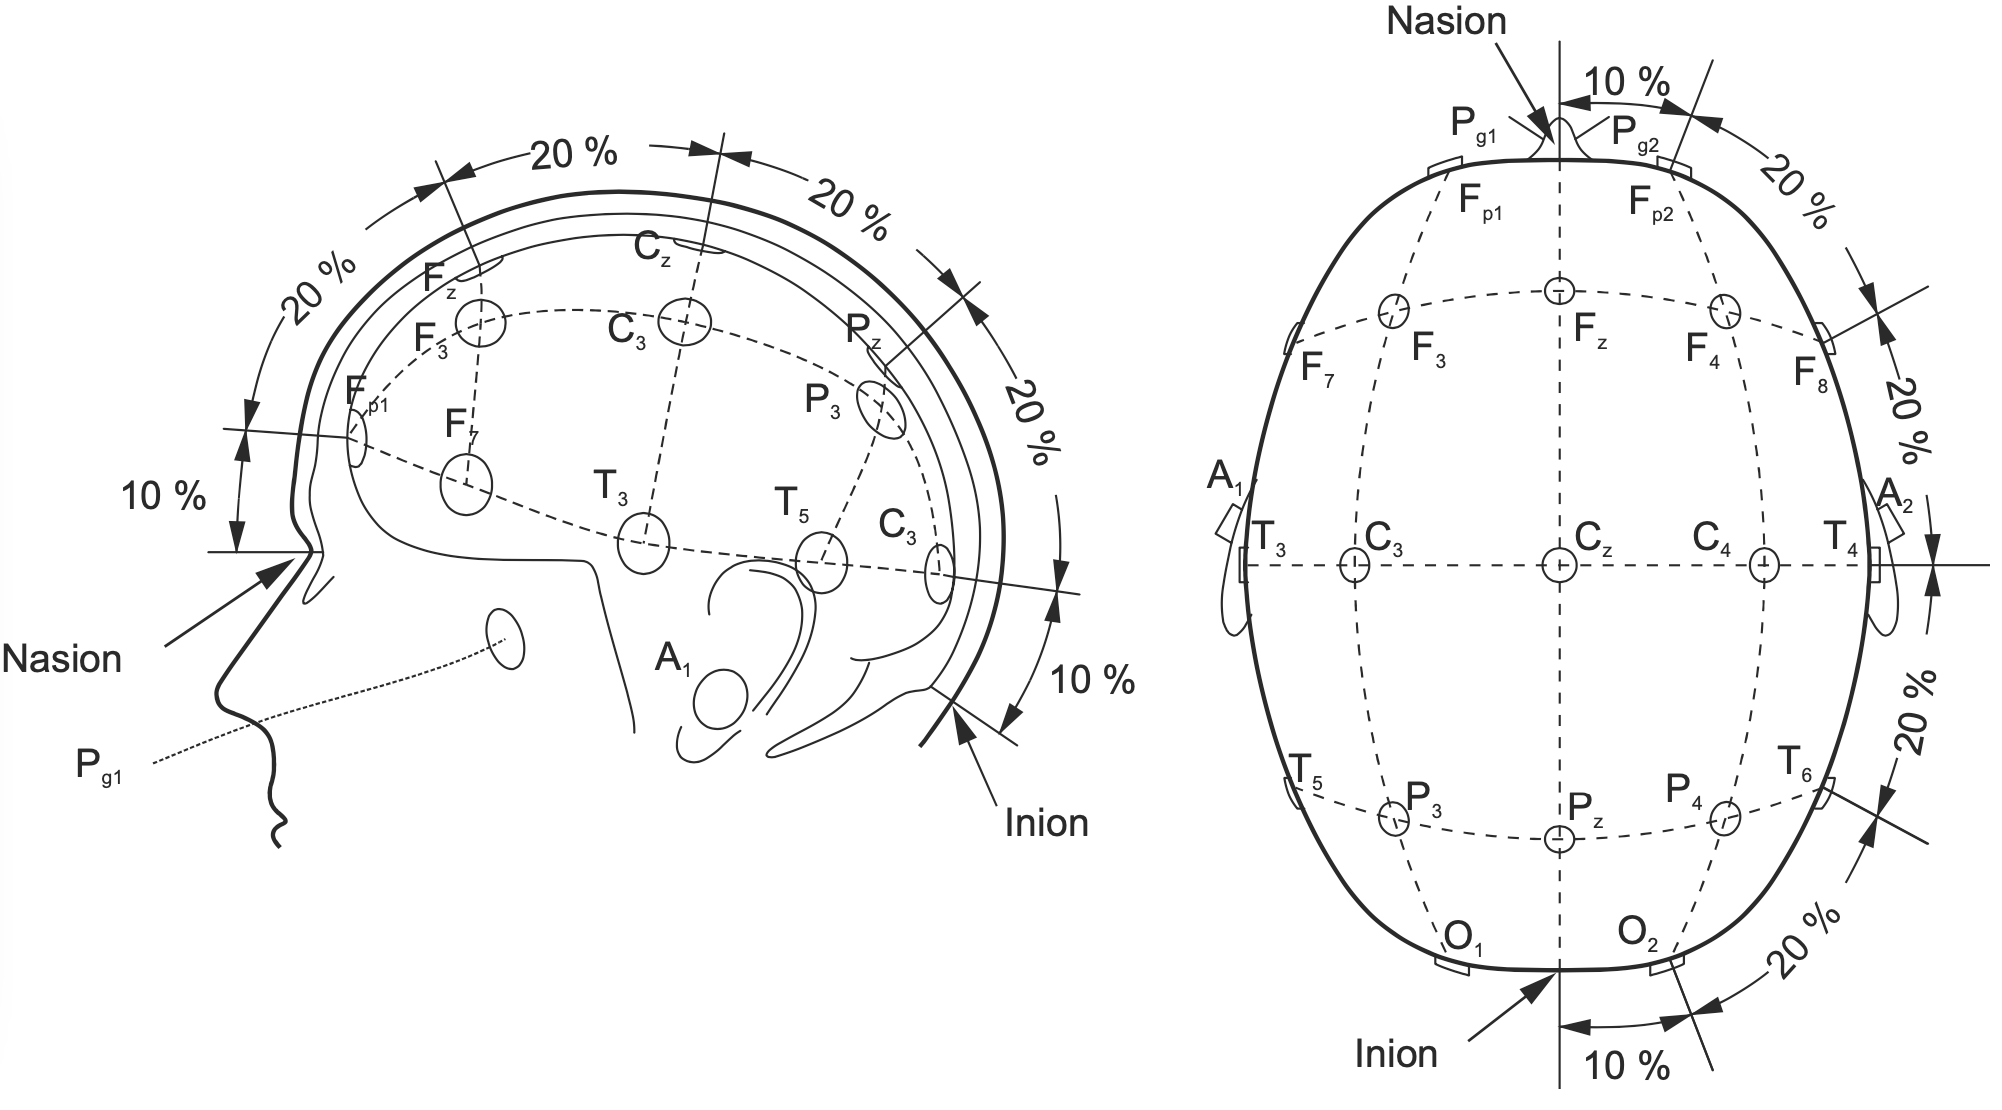
\includegraphics[width=0.8\textwidth]{10-20-electrode.png}
    \caption[Electrode positions according to the 10-20 system]{Diagram illustrating typical electrode placements using the international 10-20 system. A represents the ear lobe, C the central region, P the parietal, F the frontal and O the occipital. The \textit{naison} and \textit{inion} are used as reference locations.}
    \label{fig:10-20-positions}
\end{figure}

\subsection{BCI control signals}
The core role of a BCI is to interpret the intentions of a subject by making sense of their brain signals. These signals are comprised of a superposition of many different neuronal potentials associated with various mental tasks, most of which are not yet understood or clearly identifiable. However, there are some mental processes that have proved to correspond to identifiable signals that can be decoded by BCIs. These signals are either produced predictably in response to a particular external stimulus, or can be be modulated at will by a subject with suitable conditioning \cite{bci-survey-nicolas-alonso}. Some of the most popular BCI control signals are discussed below.

\subsubsection{Visual evoked potentials}
Visual evoked potentials (VEPs) are modulations in the activity of the brain's visual cortex in response to a visual stimulus \cite{bromm-veps}. VEPs can be characterised by the nature of the visual stimulus, namely: the flicker or reversal frequency of the, the morphology of the stimulus itself and by proportion of the visual field occupied by the stimulus \cite{bci-survey-nicolas-alonso}. Most commonly, frequency is modulated between different visual stimuli in order to encode different control targets. Transient VEPs, as the name suggests, are short-term potentials that occur in response to visual stimuli below 6Hz. Conversely, steady state VEPs (SSVEPs) are produced at frequencies above 6Hz and are characterised by sinusoidal signals with a fundamental frequency matching that of the visual stimulus \cite{Xie2016}. VEPs have the advantage of a relatively high information transfer rate (ITR) and do not require any training from the subject as they are elicited involuntarily. 

\subsubsection{Slow cortical potentials}
Slow cortical potentials (SCPs) are slow voltage shifts below 1Hz that correspond to changes in the level of cortical activity \cite{bci-survey-nicolas-alonso}. Although these signals can be self-regulated in order to control external devices through a BCI, reliable operation often requires training and is dependent on numerous external factors such as a subject's psychological state, motivation and social context \cite{bci-survey-nicolas-alonso}. Furthermore, as SCPs occur over several seconds, maximum ITRs attainable are low.

\subsubsection{Event related potentials}
Event related potentials (ERPs), such as the P300 evoked potential, are positive signal spikes generated in response to infrequent or unexpected auditory, visual or somatosensory stimuli \cite{bci-survey-nicolas-alonso}. `P300' is derived from the fact that these potentials are typically evoked around 300ms after observing an infrequent stimulus after a sequence of common or expected ones. P300-based BCIs are only capable of very low ITRs since considerable number of non-target stimuli need to be presented before the infrequent stimulus in order to preserve its novelty. Furthermore, magnitude of P300 responses may decrease with time as the subject begins to anticipate responses. 

\subsubsection{Sensorimotor rhythms}
Sensorimotor rhythms are modulations in cerebral activity associated with motor tasks, even when overt motor action is not performed. BCI control can be achieved through sensorimotor signals as subjects can be trained to generate modulations voluntarily through mental rehearsal of motor actions. For example, a subject may imagine clenching their fists. However, obtaining reliable signals through self-control proves difficult in practice as patients often imagine \textit{visual images } of related movements which does not produce sufficiently similar cerebral activity to the image of performing the actual activity itself \cite{bci-survey-nicolas-alonso}. As such, reliable BCI control usually requires special training with an emphasis on kinesthetic experiences.

\begin{table}[]
\centering
\begin{tabular}{@{}llll@{}}
\toprule
\textbf{Paradigm} &
  \textbf{Physiological phenomena} &
  \textbf{Training required} &
  \textbf{ITR (bits/min)} \\ \midrule
VEP          & \begin{tabular}[c]{@{}l@{}}Signal modulations in the visual cortex in response\\ to a flickering visual stimulus\end{tabular}     & No  & \textbf{60-200} \\
SCP          & \begin{tabular}[c]{@{}l@{}}Slow shifts in cortical potentials due to modulation\\ of cortical activity/concentration\end{tabular} & Yes & 5-12   \\
ERP &
  \begin{tabular}[c]{@{}l@{}}Abrupt signal modulations in response to infrequent\\ or unexpected stimuli\end{tabular} &
  No &
  20-25 \\
Sensorimotor & \begin{tabular}[c]{@{}l@{}}Modulations in signals from the motor cortex \\ synchronised to imagined motor actions\end{tabular}    & Yes & 3-35   \\ \bottomrule
\end{tabular}
\caption[A summary of commonly used BCI control signal paradigms]{A summary of commonly used BCI control signal paradigms. The information transfer rate (ITR) values provided are typical but may vary depending on the type of data acquisition and decoding systems used.}
\label{tab:c2-bci-control-signals}
\end{table}

\section{Steady-state visual evoked potentials (SSVEP)}
Several studies suggest that steady-state visual evoked potentials  \cite{Fernandez-Fraga2016}, \cite{Kanoga2020}, \cite{Acampora2021} (SSVEPs) offer significant potential for EEG decoding tasks similar to those in this project due to the high information transfer rate (ITR), non-invasiveness and relatively high SNR that can be achieved using basic BCI devices \cite{Zhu2021}. Moreover, SSVEP amplitudes change as a function of stimulus intensity (luminance and contrast) \cite{autthasan-single-chan-ssvep} which can easily be controlled. Considering these factors and the fact that SSVEP-based BCIs require little to no user training or prior BCI experience, it is clear that this is the most suitable EEG paradigm for this project. 

\subsection{Evoking and measuring SSVEPs}
\label{subsection:evoking-measuring-ssveps}

Broadly speaking, in order to evoke SSVEPs, flickering visual stimuli with frequencies of around 7-15Hz are commonly used \cite{Acampora2021}, \cite{Chen2017}, \cite{duart-comparing-ssvep-stimuli}, however, Xie et al demonstrated successful decoding with 27.8Hz \cite{Xie2016}. As in \cite{Acampora2021}, \cite{Chen2017}, \cite{autthasan-single-chan-ssvep}, visual stimuli are usually presented using a computer monitor with an LCD display or discrete LEDs. SSVEPs are measured in the occipital and/or parietal regions \cite{Fernandez-Fraga2016} for proximity to the visual cortex. Using the international 10-20 electrode electrode scheme, this corresponds to the parieto-occipital ($\text{PO}_x$) and occipital ($\text{O}_x$)  electrodes.

The aforementioned studies do not provide a unanimous set of parameters for the optimal SSVEP stimulus. There is substantial variation in the frequency, colour and source of stimulus used across these studies and indeed, many other studies in the literature \cite{duart-comparing-ssvep-stimuli}. Duart et al in \cite{duart-comparing-ssvep-stimuli} sought to investigate these stimulus design parameters more closely and compare their impact on accuracy of frequency discrimination and SNR (signal-to-noise ratio) in SSVEP-based BCIs. Specifically, the following parameters were tested:
\begin{itemize}
    \item \textbf{frequency}: low (5Hz), middle (12Hz) and high (30Hz) frequencies were tested.
    \item \textbf{colour}: red, white and green squares were experimented with. 
    \item \textbf{attention}: a measure of attention was tested using to determine correlation with evoked responses.
\end{itemize}
Duart et al found that the middle frequency of 12Hz produced maximal SNR, followed by the low 5Hz frequency. Furthermore, red and green stimuli produced responses with maximum SNR at 5Hz while red and white were optimal at 12Hz. No difference in SNR was observed between colours at 30Hz. Despite red light proving optimal in other studies such as \cite{chu-ssvep-colours}, Duart et al note that red light may produce increased risk of inducing epileptic seizures and should thus be avoided where possible. Moreover, Zhu et al noted that lower (flicker) frequencies and light colours of longer wave length tend to produce greater visual fatigue which consequently degrades SSVEP responses over time \cite{zhu2010survey}. Finally, Duart et al measured attention of subjects undergoing SSVEP trials through the Conner's Continuous Performance Task version 2 (CPT-II) which measures reaction times, omission errors and commission errors \cite{duart-comparing-ssvep-stimuli}. They found that this measure of attention showed a significant correlation to the SNR of evoked SSVEP signals at the low frequency of 5Hz, but less so with higher frequencies. The authors hypothesised that this may be due to the fact that greater concentration is required at lower frequencies that cause greater fatigue \cite{duart-comparing-ssvep-stimuli}.

Taking into account these findings, it would appear that using stimulus frequencies of around 12Hz would be a suitable choice. Furthermore, so as to avoid using red light, white would be a good choice in medium frequency range and green would be suitable for lower frequencies around 5Hz. Using frequencies around 12Hz has the added advantage of causing less visual fatigue and theoretically, should require less active concentration from subjects in order to achieve adequate SNR.

\subsubsection{Electrode placement}

\subsubsection{Time-frequency considerations}
\label{subsection:time-frequency-considerations-c2}
Mention typical time windows required for accurate performance and how/if sliding windows are implemented. 

Mention breaks between trials or any other things done between presentation of stimuli

Also mention typical samplign rates and implications on number of harmonics we can include etc. 

Mention typical filtering choices - e.g. bandpass + 50Hz notch

% Decoding algos section
\section{Computational Approaches for SSVEP Decoding}
\subsection{Power spectral density and frequency domain}
\subsection{Statistical}

\subsubsection{Canonical correlation analysis (CCA)}
\label{subsection:CCA-c2}
CCA is a standard multivariate statistical technique for analysing multiple variables measured on a set of observations. In particular, variables are partitioned into two sets or \textit{views} of the data \cite{cca-tutorial}. Effectively, CCA is a multivariate extension of ordinary correlation. Given variable partitions $\mX \in \R^{m\times p}$, $\mY \in \R^{m\times q}$ each with $m$ observations, CCA seeks to find a linear combination of $\mX$, $\mY$ that maximises the correlation between their images $\vz_X = \mX\vw_X$ and $\vz_Y = \mY\vw_Y$. These images are known as the \textit{canonical variables} and $\vw_X$ and $\vw_Y$ are the \textit{canonical weight vectors} that effectively act as spatial filters across signal channels.

With CCA for SSVEP frequency recognition tasks, $\mX \in \R^{N_s\times N_c}$ is the set of \textit{measured} EEG signals from $N_c$ channels over $N_s$ observations. The measured signals in $\mX$ must be compared with each frequency $f_k \in \mathcal{F}$, a finite set of candidate stimulus frequencies. CCA can be used to compute weighted correlations between the measured signals and each candidate frequency $f_k$ by constructing a sinusoidal reference signal set $\mY_k \in \R^{N_s \times 2N_h}$ as follows: 
\begin{equation}
\mY_{k}=\left(\begin{array}{c}
\sin \left(2 \pi f_{k} t\right) \\
\cos \left(2 \pi f_{k} t\right) \\
\sin \left(4 \pi f_{k} t\right) \\
\cos \left(4 \pi f_{k} t\right) \\
\vdots \\
\sin \left(2 \pi N_h f_{k} t\right) \\
\cos \left(2 \pi N_h f_{k} t\right)
\end{array}\right), \quad t=\frac{1}{f_s}, \frac{2}{f_s}, \ldots, \frac{N_s}{f_s}
\label{eq:sinusoidal-ref}
\end{equation}
where $f_s$ is the sampling frequency and $N_h$ is the number of harmonics in the reference set, a parameter to be chosen. The scalp and other interacting layers between the brain and surface electrodes are both resistive and capacitive, producing low-pass filter dynamics \cite{baillet-em-brain-mapping}, \cite{lin-cca-2006}. Therefore, it is rare that more than $N_h=5$ harmonics are selected in the reference signal set \cite{lin-cca-2006}. The final task of frequency recognition is performed by selecting the frequency $f^*$
\begin{equation}
    f^* = \argmax_{f_k} \; \rho_k, \quad \forall \, f_k \in \mathcal{F}
    \label{eq:cca-freq-discrimination}
\end{equation}
corresponding to the candidate frequency $f_k$ which maximises the canonical correlation $\rho_k$ between $\mX$ and the the reference set $\mY_k$. While standard CCA is a good starting point for statistical SSVEP decoding as it forms the basis of many similar algorithms, there are several extensions which have been shown to improve signal recognition performance \cite{zhang-mset-cca}, \cite{sun-gcca}, \cite{miao-hybrid-cca}. The most promising of these are explored below.

\subsubsection{Task-related component analysis (TRCA)}
\label{section:trca-c2}
Task-related component analysis (TRCA) as a decoding technique in biophysical systems was introduced in the seminal paper by Tanaka et al \cite{tanaka-trca}. TRCA seeks to extract task-related signal components (as opposed to spurious, unwanted components such as EMG artefacts and background noise) by identifying components that lead to maximum reproducibility across trials. Task-related components are constructed as linear combinations of signals recorded across multiple time blocks (trials) and their weights are optimised so as to maximise their inter-block correlation or covariance \cite{tanaka-trca}. Components with maximum inter-block covariance and thus, reproducibility or consistency, are identified as task-related components (subject to certain significance measures as discussed later). Further advantages of TRCA are that, unlike other more common generalised linear models (GLMs), it assumes no \textit{a priori} knowledge of source signals and is not sensitive to autocorrelation \cite{tanaka-trca}. It also offers concrete measures of task-relatedness unlike some other data-driven methods like independent component analysis.

To illustrate the basic idea of this algorithm, \cite{tanaka-trca} presents a useful toy example. Consider a task-related signal $s(t)$ standardised to have zero mean and unit variance embedded in additive white (uncorrelated) noise $n(t)$: $x(t) = a_1s(t) + a_2n(t)$ with some mixing scalars $a_i \in \R$. Then, assume the observable signal $x(t)$ is measured over two distinct blocks or trials to yield $x_1(t)$ and $x_2(t)$. A linear model of the two observed blocks could be defined as follows:
\begin{align}
    x_1(t) = a_{11}s(t) + a_{12}n(t) \\
    x_2(t) = a_{21}s(t) + a_{22}n(t) \\
\end{align}
As mentioned above, TRCA attempts to recover task related components (only $s(t)$ in this case) from a linear combination of observations across trials. Defining this weighted sum as $y(t)$ with 
\begin{equation}
    y(t)= y_1(t) + y_2(t) = w_{1} x_{1}(t)+w_{2} x_{2}(t)=\left(w_{1} a_{11}+w_{2} a_{21}\right) s(t)+\left(w_{1} a_{12}+w_{2} a_{22}\right) n(t)
\end{equation}
Recovering $s(t)$ involves maximising the covariance between $y_1(t)$ and $y_2(t)$:
\begin{align}
\begin{split}
\operatorname{Cov}\left(y_1, y_2\right)=&\left(w_{1} a_{11}+w_{2} a_{21}\right)^{2} \operatorname{Cov}\left(s_1, s_2\right)
+\left(w_{1} a_{12}+w_{2} a_{22}\right)^{2} \operatorname{Cov}\left(n_{1}, n_2\right) \\
&+\left(w_{1} a_{11}+w_{2} a_{21}\right)\left(w_{1} a_{12}+w_{2} a_{22}\right)\left[\operatorname{Cov}\left(s_{2}, n_2\right)\right
\left.+\operatorname{Cov}\left(n_{1}, s_2\right)\right]
\end{split}
\\
\notag
=&\left(w_{1} a_{11}+w_{2} a_{21}\right)^{2} \operatorname{Cov}\left(s_{1}, s_2\right)
\end{align}
Since $\operatorname{Cov}(n_1, n_2) = \operatorname{Cov}(s_1, n_2) = \operatorname{Cov}(n_1, s_2) = 0$. In order to bound this quadratic objective, we choose the weights $w_1, w_2$ so that the variance of $y$ is constrained to 1:
\begin{equation}
    \operatorname{var}(y)=\left(w_{1} a_{11}+w_{2} a_{21}\right)^{2}+\left(w_{1} a_{12}+w_{2} a_{22}\right)^{2}=1
\end{equation}
where $s(t)$ and $n(t)$ are also assumed to be uncorrelated $\forall t$. The solution of this constrained optimisation problem is 
\begin{equation}
    w_{1} a_{11}+w_{2} a_{21} = 1, \quad w_{1} a_{12}+w_{2} a_{22} = 0, 
\end{equation}
which, barring the unlikely case that $a_{11}a_{22} = a_{12}a_{21}$, yields $y(t)=s(t)$ as desired. This demonstrates how inter-trial covariance maximisation can be used for recovery of task-related signals.

Although TRCA has been shown to outperform CCA \cite{lee-trca-2step}, \cite{miao-hybrid-cca}, \cite{sun-gcca}, extended and hybrid forms of these algorithms have produced superior results. Some of these extensions are explored below.

\subsubsection{Multiset canonical correlation analysis (MsetCCA)}
MsetCCA is one extension of standard CCA that takes into account historical data instead of performing inference purely on new observations. Zhang et al propose that this is one of the reasons that standard CCA performs poorly on short time windows; it effectively over fits to localised dynamics \cite{zhang-mset-cca}. Furthermore, the authors suggest that exclusively using the pre-constructed sinusoidal reference set is not optimal since this artificial reference does not exclude other features from real EEG data \cite{zhang-mset-cca}. To circumvent this, MsetCCA seeks to optimise the reference signals used in the CCA algorithm by learning multiple linear transforms to maximise overall correlation between canonical variables over \textit{many} sets of EEG data at each candidate frequency $f_k \in \mathcal{F}$ \cite{zhang-mset-cca}. This optimisation effectively finds optimal joint spatial filters $\vw_1, \dots, \vw_{N_t}$ (over $N_t$ trials) using only historical observations (`training' data). The authors claim that MsetCCA outperforms similar techniques, especially in cases with few channels and short time windows. 

\subsubsection{Generalised canonical correlation analysis (GCCA)}
Wong et al noted in their study of EEG spatial filtering methods in \cite{wong-spatial-filt} that only using historical observations to estimate spatial filters (canonical weights) $\vw_i$, as in MsetCCA, is not optimal. Using both historical data and pre-constructed sinusoidal reference signals as with standard CCA was found to enhance the algorithm's robustness and reduced calibration requirements \cite{wong-spatial-filt}.  Motivated by this, the authors in \cite{sun-gcca} developed a new algorithm called generalised CCA (GCCA) that aims to simultaneously maximise correlation between three sets of data: historical observations, measured signals in a new sample and the pre-constructed sinusoidal reference. As interpreted by the authors in \cite{sun-gcca}, the optimal spatial filters obtained through GCCA perform SSVEP signal denoising.

\subsection{Data-driven and machine learning}

% % Chapter 3: Theory Development
% % Chapter 3: Theory Development
\chapter{Theory Development}
\label{chapter:theory-development}

\graphicspath{ {report/C3 Theory Development/assets/} } 

\section{Theoretical Development of SSVEP Decoding Algorithms}

\subsection{Canonical correlation analysis (CCA)}
\label{section:cca-c3}
Given variable partitions $\mX \in \R^{m\times p}$, $\mY \in \R^{m\times q}$ each with $m$ observations, CCA seeks to find a linear combination of $\mX$, $\mY$ that maximises the correlation between their images. More formally, assuming that the variables (columns) of the two partitions $\vx_1, \dots, \vx_p \in \R^{m}$ and $\vy_1, \dots, \vy_q \in \R^{m}$ are standardised to have zero mean and unit variance, find
\begin{align}
    \rho &= \max_{\vw_X, \vw_Y} \textrm{corr}(\mX \vw_X, \mY \vw_Y) \\
    &= \max_{\vw_X, \vw_Y} \frac{\E[\mX \vw_X\vw_Y^\top\mY^\top ]}{\sqrt{\E[\mX \vw_X\vw_X^\top\mX^\top]\E[\mY \vw_Y\vw_Y^\top\mY^\top]}}
    \label{eq:cca-corr-objective}
\end{align}
where $\rho$ is the \textit{canonical correlation}, $\vw_X$ and $\vw_Y$ are the canonical weight vectors and the images $\vz_X = \mX\vw_X$ and $\vz_Y = \mY\vw_Y$ are the \textit{canonical variables} for $\mX$ and $\mY$ respectively.

\subsubsection{Geometric interpretation}
The authors in \cite{cca-tutorial} present an intuitive geometric analogy. Consider $\mX$ and $\mY$ as linear transforms of position vectors $\vw_X$ and $\vw_Y$ onto their images $\vz_X$ and $\vz_Y$ in $\R^m$. CCA constrains $\vz_X$ and $\vz_Y$ to have unit norm and that the angle $\theta \in [0, \frac{\pi}{2}]$ between them be minimised so as to maximise their correlation. The canonical correlation $\rho$ is then the inner product of $\vz_X$ and $\vz_Y$:
\begin{equation}
    \rho = \vz_X^\top\vz_Y = \|\vz_X\| \|\vz_Y\|\cos(\theta) = \cos(\theta)
\end{equation}
Therefore, CCA aims to find position vectors $\vw_X$, $\vw_Y$ that, after undergoing linear transforms $\mX$ and $\mY$, are mapped to a unit sphere in $\R^m$ where $\theta$ is minimised \cite{cca-tutorial}. Note that there will be $n=\textrm{min}(p, q)$ canonical correlations $\rho_1, \dots, \rho_n$ with $|\rho_i| \geq |\rho_j|, \; \forall \; i < j$. Typically, only the first and largest canonical correlation $\rho_1$ is considered. 

\subsubsection{Solving for canonical weight vectors through the eigenvalue problem}
Consider the case of solving for the first and largest canonical correlation $p_1$. Following the geometric interpretation, the objective is to find
\begin{equation}
    \cos(\theta_1) = \max_{\vw_X, \vw_Y}\langle\,\vz_X,\vz_Y\rangle \quad \textrm{with} \quad \|\vz_X\| = \|\vz_Y\| = 1
\label{eq:cca-objective-1}
\end{equation}
where $\theta_1$ is the smallest angle between image vectors. Defining the within-set covariance matrices as 
\begin{align}
    \mC_{XX} = \mX^\top\mX \quad \textrm{and} \quad
    \mC_{YY} = \mY^\top \mY 
\end{align}
and the inter-set cross covariance matrix as 
\begin{align}
    \mC_{XY} &= \mX^\top\mY,
\end{align}
the unit variance constraint on the image vectors can be rewritten as  \begin{align}
\begin{split}
    \|\vz_X\| &= \vz_X^\top\vz_X = \vw_X^\top \mX^\top \mX \vw_X =  \vw_X^\top \mC_{XX} \vw_X = 1 \\
    \|\vz_Y\| &= \vz_Y^\top\vz_Y = \vw_Y^\top \mY^\top \mY \vw_Y =  \vw_Y^\top \mC_{YY} \vw_Y = 1 
    \end{split}
\label{eq:unit-variance-reformulated}
\end{align}
Substituting (\ref{eq:unit-variance-reformulated}) into (\ref{eq:cca-corr-objective}) yields 

\begin{equation}
\cos(\theta) = \max_{\vw_X, \vw_Y} \vw_X^\top \mC_{XY} \vw_Y 
\end{equation}
Lagrangian dual theory provides a straight forward way to solve the constrained optimisation problem above with unit variance constraints as in (\ref{eq:unit-variance-reformulated}). Consider the Lagrangian for this problem below with Lagrange multipliers $\lambda_1$ and $\lambda_2$:
\begin{equation}
    \mathcal{L}(\vw_X, \vw_Y, \lambda_1, \lambda_2) = \vw_X^\top \mC_{XY} \vw_Y - \frac{\lambda_1}{2}(\vw_X^\top \mC_{XX} \vw_X-1) - \frac{\lambda_2}{2}(\vw_Y^\top \mC_{YY} \vw_Y-1)
\end{equation}
With reference to the KKT conditions, stationary requires
\begin{align}
    \label{eq:cca-lagrange-x}
    \frac{\partial \mathcal{L}}{\partial \vw_X} &= \mC_{XY} \vw_Y - \lambda_1\mC_{XX} \vw_X = 0 \\
    \frac{\partial \mathcal{L}}{\partial \vw_Y} &= \mC_{YX} \vw_X - \lambda_2\mC_{YY} \vw_Y = 0
        \label{eq:cca-lagrange-y}
\end{align}
Since $\mC_{YX} = \mC_{XY}^\top$. Pre-multiplying (\ref{eq:cca-lagrange-x}) by $\vw_X^\top$ and (\ref{eq:cca-lagrange-y}) by $\vw_Y^\top$ yields:
\begin{align}
\begin{split}
    \vw_X^\top\mC_{XY} \vw_Y - \lambda_1\vw_X^\top\mC_{XX} \vw_X &= 0 \\
    \vw_Y^\top\mC_{YX} \vw_X - \lambda_2\vw_Y^\top\mC_{YY} \vw_Y &= 0
\end{split}
\label{eq:lagrange-multi}
\end{align}
Since $\vw_X^\top \mC_{XX} \vw_X = \vw_Y^\top \mC_{YY} \vw_Y =1$, it is clear from (\ref{eq:lagrange-multi}) that $\lambda_1=\lambda_2 = \lambda$. Substituting this result into (\ref{eq:cca-lagrange-x}) yields
\begin{align}
    \vw_X = \frac{\mC_{XX}^{-1}C_{XY}\vw_Y}{\lambda}
\end{align}
Then, substituting into (\ref{eq:cca-lagrange-y}) produces the following generalised eigenvalue problem:
\begin{align}
    \mC_{YX}\mC^{-1}_{XX}\mC_{XY}\vw_{Y} = \lambda^2\mC_{YY}\vw_Y
\end{align}
If $\mC_{YY}$ is non-singular, this reduces to a standard eigenvalue problem of the form
\begin{align}
    \mC_{YY}^{-1}\mC_{YX}\mC^{-1}_{XX}\mC_{XY}\vw_{Y} = \lambda^2\vw_Y
\end{align}
The eigenvalues of the matrix $\mC_{YY}^{-1}\mC_{YX}\mC^{-1}_{XX}\mC_{XY}$ correspond to the squares of the canonical correlations $\rho_1, \dots, \rho_n$.

\subsection{Task-related component analysis (TRCA)}
\label{sec:trca-c3}
Expanding from the toy example in Section \ref{section:trca-c2}, the TRCA algorithm implicitly assumes that observed signals are generated as a linear combination of task-related and task-unrelated components which implies that task-related components can be recovered by applying an appropriate weighting of observed signals across trials \cite{tanaka-trca}. Inter-trial covariance maximisation is the core objective that aims to extract task-related components with maximal temporal similarity across trials. 

Now that multiple trials are to be considered, the signal matrix $\mX\in \R^{N_s \times N_c}$ introduced in Section \ref{section:cca-c3} must be extended to a third order signal tensor $\tX \in \R^{N_s \times N_c \times N_t}$ with $N_t$ trials, each with $N_c$ channels\footnote{the constraint that the number of variables (width of $\mX_i$) for each trial be constant is not strictly necessary. For this application, however, it is assumed that the number of channels will not change between trials of a given experiment.} and $N_s$ samples. Let $\vy^{(k)}$ be the $k$-th trial (block) with $k\in\{1, 2, \dots, N_t\}$ of the signal $y(t)$ and $\vx_i^{(k)}$ be the $k$-th trial of the input signal from channel $i, \, i\in\{1, \dots, N_c\}$. Consider the covariance between all $i$ channels for two trials $k$ and $l$:

\begin{equation}
    \widehat{\mC}_{k l}=\operatorname{Cov}\left(\vy^{(k)}, \vy^{(l)}\right)=\sum_{i, \, j=1}^{N_c} w_{i} w_{j} \operatorname{Cov}\left(\vx_{i}^{(k)}, \vx_{k}^{(l)}\right)
\end{equation}
Furthermore, as with CCA, we must impose the constraint on the designed weights such that the variance of $y(t)$ is bounded:
\begin{equation}
    \operatorname{Var}(\vy)=\sum_{i, \, j=1}^{N_c} w_{i} w_{j} \operatorname{Cov}\left(\vx_{i}, \vx_{j}\right)=\mathbf{w}^{\mathrm{T}} \mQ \mathbf{w}=1
\end{equation}
Then, all possible combinations of trials $1, \dots, N_t$ are summed as
\begin{align}
\begin{split}
\sum_{\substack{k, \, l=1, \\ k\neq l}}^{N_t} \widehat{\mC}_{k l} &=\sum_{\substack{k, \, l=1, \\ k\neq l}}^{N_t} \operatorname{Cov}\left(\vy^{(k)}, \vy^{(l)}\right) \\
& =\sum_{\substack{k, \, l=1, \\ k\neq l}}^{N_t} \sum_{i, j=1}^{N_c} w_{i} w_{j} \operatorname{Cov}\left(\vx_{i}^{(k)}, \vx_{j}^{(l)}\right)= \vw^\top \mS \vw
\end{split}
\label{eq:trca-cov-sum}
\end{align}
where $\mS$ is the following symmetric matrix
\begin{equation}
    \mS_{i, j} = \sum_{\substack{k, \, l=1, \\ k\neq l}}^{N_t} \operatorname{Cov}\left(\vx_{i}^{(k)}, \vx_{j}^{(l)}\right)
\end{equation}
As alluded to before, (\ref{eq:trca-cov-sum}) yields the sum of covariances of all combinations of trials: a measure of task consistency. This is precisely what we want to maximise. This constrained optimisation problem (recalling the variance constraint on $y(t)$) can be reformulated as a Rayleigh-Ritz eigenvalue problem of the form 

\begin{equation}
    \vw^*=\underset{\vw}{\arg \max } \frac{\vw^\top \mS \vw}{\vw^\top \mQ \vw}
\label{eq:trca-rayleigh-ritz}
\end{equation}
The inter-trial weight vectors $\vw_k, \, k \in \{1, \dots, N_t\}$ can be found by computing the eigenvectors of $\mQ^{-1}\mS$. Specifically, the degree of task-relatedness corresponds to the magnitude of the eigenvalues of $\mQ^{-1}\mS$ and so the optimal weight $\vw^*$ corresponds to the largest eigenvalue.

\subsection{Multiset CCA (MsetCCA)}
MsetCCA is an extension of standard CCA to multiple data sets or partitions. Accordingly, the objective is now to maximise the correlation between canonical variables from \textit{many sets} of observations at a given stimulus frequency $f_k$. Although several objective functions for MsetCCA exist, the MAXVAR objective is explored in \cite{zhang-mset-cca} for its intuitive extension to ordinary CCA with multiple variable sets. Assuming all sets of variables in $\tX$ are normalised to have zero mean and unit variance, the MAXVAR objective for maximising correlation over canonical variables from multiple sets at a given candidate frequency $f_k$ is defined as follows:
\begin{align}
\begin{split}
\max_{\mathbf{w}_{1}, \ldots, \mathbf{w}_{N_t}} & \quad \rho=\sum_{i \neq j}^{N_t} \mathbf{w}_{i}^\top\mX_{i}^\top \mX_{j}\mathbf{w}_{j} \\
\text { s.t. } & \quad \frac{1}{N_t} \sum_{i=1}^{N_t} \mathbf{w}_{i}^\top\mX_{i}^\top \mX_{i}\mathbf{w}_{i}=1,
\end{split}
\label{eq:mset-cca-objective}
\end{align}
where the same conventions for the signal tensor $\tX$ as in Section \ref{sec:trca-c3} above apply. Following a similar approach as in the derivation for CCA above, the method of Lagrange multipliers can be used to transform the constrained optimisation problem in (\ref{eq:mset-cca-objective}) to a generalised eigenvalue problem of the form:
\begin{equation}
        (\mR -\mS)\vw = \rho\mS \vw
\label{eq:mset-cca-gen-eig}
\end{equation}
where
\begin{align*}
\mR = \begin{bmatrix}
\mX_{1}^{\top}\mX_{1} & \ldots & \mX_{1}^{\top}\mX_{N_t} \\
\vdots & \ddots & \vdots \\
\mX_{N_t}^{\top}\mX_{1} & \ldots & \mX_{N_t}^{\top} \mX_{N_t}
\end{bmatrix},
\quad
\mS = \begin{bmatrix}
\mX_{1}^{\top}\mX_{1} & \ldots & 0 \\
\vdots & \ddots & \vdots \\
0 & \ldots & \mX_{N_t}^{\top} \mX_{N_t}
\end{bmatrix}
\quad
\textrm{and}
\quad
\vw = \begin{bmatrix}
\vw_1 \\ \vdots \\ \vw_{N_t}
\end{bmatrix}
\end{align*}
Thus, $\mR$ is the inter-trial block covariance matrix which captures sub-covariance matrices between all pairs of trials $n\in \{1, \dots, N_t \}$. $\mS$ is a block diagonal matrix which captures within-set covariance matrices for each trial. $\vw$ is a matrix of optimal spatial filters (vectors) $\vw_1, \dots, \vw_{N_t}$ resulting from the largest combined canonical correlation between all canonical variables $\vz_i = \mX_i\vw_i \in \R^{N_s}, \; \forall \; i\in[1, \; N_t]$. As with standard CCA, the largest canonical correlation $\rho^*$ corresponds to the largest generalised eigenvalue in (\ref{eq:mset-cca-gen-eig}). The canonical variables $\vz_i$ corresponding to $\rho^*$ are indeed the eigenvectors corresponding to the largest generalised eigenvalue \cite{zhang-mset-cca}. The optimal reference $\mY_k \in \R^{N_s \times N_t}$ for given frequency $f_k$ can be computed using the spatial filters from $\vw$ as:
\begin{align}
    \mY_k =
    \begin{bmatrix}
    \vz_{1, \, k} & \dots & \vz_{N_t, \,k}
    \end{bmatrix}
    =
    \begin{bmatrix}
    \mX_{1, \, k}\vw_{1, \, k}  & \dots & \mX_{N_t, \,k}\vw_{N_t,\, k} 
    \end{bmatrix}
\end{align}

After this training or calibration process is complete and $\mY_k$ is computed for all candidate frequencies $f_k$, these optimised reference sets can be used for inference. Given a new set of test signals $\hat{\mX} \in \R^{N_s \times N_c}$, ordinary CCA as in Section \ref{section:cca-c3} can be used to discern the frequency $f^*$ corresponding to the highest canonical correlation between $\hat{\mX}$ and the associated referenced set $\mY^*$. The process for finding $f^*$ is identical to that in (\ref{eq:cca-freq-discrimination}). The important difference here is how the pre-computed reference sets $\mY_k$ used in the CCA algorithm are calculated.

\subsection{Generalised CCA (GCCA)}
Consider a single candidate frequency $f_k$: for the rest of this subsection, the $k$ index is ommitted for brevity but all symbols refer to those specific to the single set of trials for $f_k$. As with MsetCCA, GCCA requires a signal tensor $\tX \in \R^{N_s \times N_c \times N_t}$ that incorporates several trials. The \textit{template matrix} $\overline{\mX}$ is obtained by computing the arithmetic mean of all trials in the set: $\overline{\mX}= \frac{1}{N_t}\sum_{i=1}^{N_t}\tX_{i}$. The concatenated signal matrix $\mX^{c}$ is formed by unrolling $\tX$ along the third (trial) axis:
\begin{equation}
    \mX^{c} = \begin{bmatrix}
    \mX_1^\top & \mX_2^\top & \dots & \mX_{N_t}^\top
    \end{bmatrix} \in \R^{N_c \times (N_s N_t)} 
\end{equation}
Then, the template and sinusoidal reference matrices are concatenated similarly to match the dimensions of  
$\mX^{c}$:
\begin{equation}
    \overline{\mX}^{c} = \begin{bmatrix}
    \overline{\mX}^\top & \overline{\mX}^\top & \dots & \overline{\mX}^\top
    \end{bmatrix} \in \R^{N_c \times (N_s N_t)} \quad \textrm{and} \quad  \mY^{c} = \begin{bmatrix}
    \mY^\top & \mY^\top & \dots & \mY^\top
    \end{bmatrix} \in \R^{2N_h \times (N_s N_t)}
\end{equation}
where $\mY$ follows the definition of the sinusoidal reference in (\ref{eq:sinusoidal-ref}). Consider the augmented spatial filter vector $\widetilde{\vw}$: 
\begin{equation}
\widetilde{\vw} = \begin{bmatrix}\vw_{\mX^{c}} & \vw_{\overline{\mX}^{c}} & \vw_{\mY^{c}} \end{bmatrix}^\top 
\end{equation}
Similarly, the augmented signal matrix $\widetilde{\mX}$ is defined as: 
\begin{equation}
\widetilde{\mX} = \begin{bmatrix}(\mX^{c})^\top & (\overline{\mX}^{c})^\top & (\mY^{c})^\top \end{bmatrix}^\top
\end{equation}
The objective of GCCA can then be expressed as
\begin{align}
\begin{split}
    \textrm{maximise} & \quad \textrm{tr}(\widetilde{\vw}^\top\widetilde{\mX}\widetilde{\mX}^\top\widetilde{\vw}) \\
    \textrm{s.t.} & \quad \widetilde{\vw}^\top\mD\widetilde{\vw} = \mI
\end{split}
\label{eq:gcca-objective}
\end{align}
where $\mD$, the within-set block covariance matrix, is defined as 
\begin{equation}
    \mD = \begin{bmatrix}
    \mX^{c}(\mX^{c}})^\top & 0 & 0 \\
    0 & \overline{\mX}^{c}(\overline{\mX}^{c})^\top & 0 \\
    0 & 0 & \mY^{c}(\mY^{c}})^\top
    \end{bmatrix}
\end{equation}
Again, using the method of Lagrange multipliers, (\ref{eq:gcca-objective}) can be reformulated as a generalised eigenvalue problem of the form
\begin{equation}
    \widetilde{\mX}\widetilde{\mX}^\top\widetilde{\vw} = \lambda\mD\widetilde{\vw} 
    \label{eq:gcca-D}
\end{equation}
If $\mD$ is non-singular, (\ref{eq:gcca-D}) resolves to an ordinary eigenvalue problem:
\begin{equation}
    \mD^{-1}\widetilde{\mX}\widetilde{\mX}^\top\widetilde{\vw} = \lambda\widetilde{\vw} 
    \label{eq:gcca-D-standard}
\end{equation}
Then, the eigenvector of $\mD^{-1}\widetilde{\mX}\widetilde{\mX}^\top$ corresponding to its largest eigenvalue is the optimal spatial filter $\vw^* \in \R^{2(N_c+N_h)}$. 

Given a new test sample set $\hat{\mX} \in \R^{N_s\times N_c}$, two correlations are computed: first between the test data and the historical template, and then between the test data and sinusoidal reference. This can be expressed as 
\begin{align}
    \rho_1 &= \textrm{corr}(\hat{\mX}\vw_{\mX^{c}}, \; \overline{\mX}\vw_{\overline{\mX}^{c}}) \\
    \rho_2 &= \textrm{corr}(\hat{\mX}\vw_{\mX^{c}}, \; \mY\vw_{\mY^{c}}) 
\end{align}
where Pearson's correlation is denoted by \textit{corr}. Finally, the output correlation for frequency $f_k$ is computed as a combination of $\rho_1$ and $\rho_2$:
\begin{equation}
    \rho = \textrm{sign}(\rho_1)\rho_1^2 + \textrm{sign}(\rho_2)\rho_2^2
\end{equation}


\subsection{Related theory}
\subsubsection{Significance testing}
\subsubsection{Quantifying signal quality}
\subsubsection{Mechanics of sampling}

% % Chapter 4: Apparatus and experimental procedure
% % Chapter 4: Experimental Procedure 
\chapter{Apparatus and Experimental Procedure}
\label{chapter:experimental-procedure}

\graphicspath{ {report/C4 Experimental Procedure/assets/} } 

\section{BCI Apparatus}

In general, EEG-based BCI systems are comprised of the following core elements \cite{teplan-eeg-measurement}, \cite{bci-survey-nicolas-alonso}:
\begin{itemize}
    \item electrodes: placed on the scalp of the subject to record raw electrical potentials. 
    \item signal processing elements: amplifiers and filters are typically employed before the signals are digitised
    \item analogue-to-digital converter (ADC): digitises measured signal for manipulation in a computer or microcontroller
    \item computer or microcontroller: facilitates data processing, computation and storage
\end{itemize}

\subsection{OpenBCI Ganglion}
As the Imperial NGNI hardware prototype was still under development for a large part of this project, experimentation was initially done on a Ganglion bio-sensing kit made by \href{https://shop.openbci.com/products/ganglion-board?variant=13461804483}{OpenBCI} (OpenBCI, New York, USA). This kit was chosen due to the fact that it is relatively low-cost at 374.99 USD, open-source and has been scientifically validated as in \cite{autthasan-single-chan-ssvep}, \cite{peterson-bci-survey}. Furthermore, it is a relatively simple platform with sensing capabilities that are likely the most comparable to those anticipated for the NGNI prototype.

\begin{figure}
     \begin{subfigure}[c]{0.45\textwidth}
         \centering
         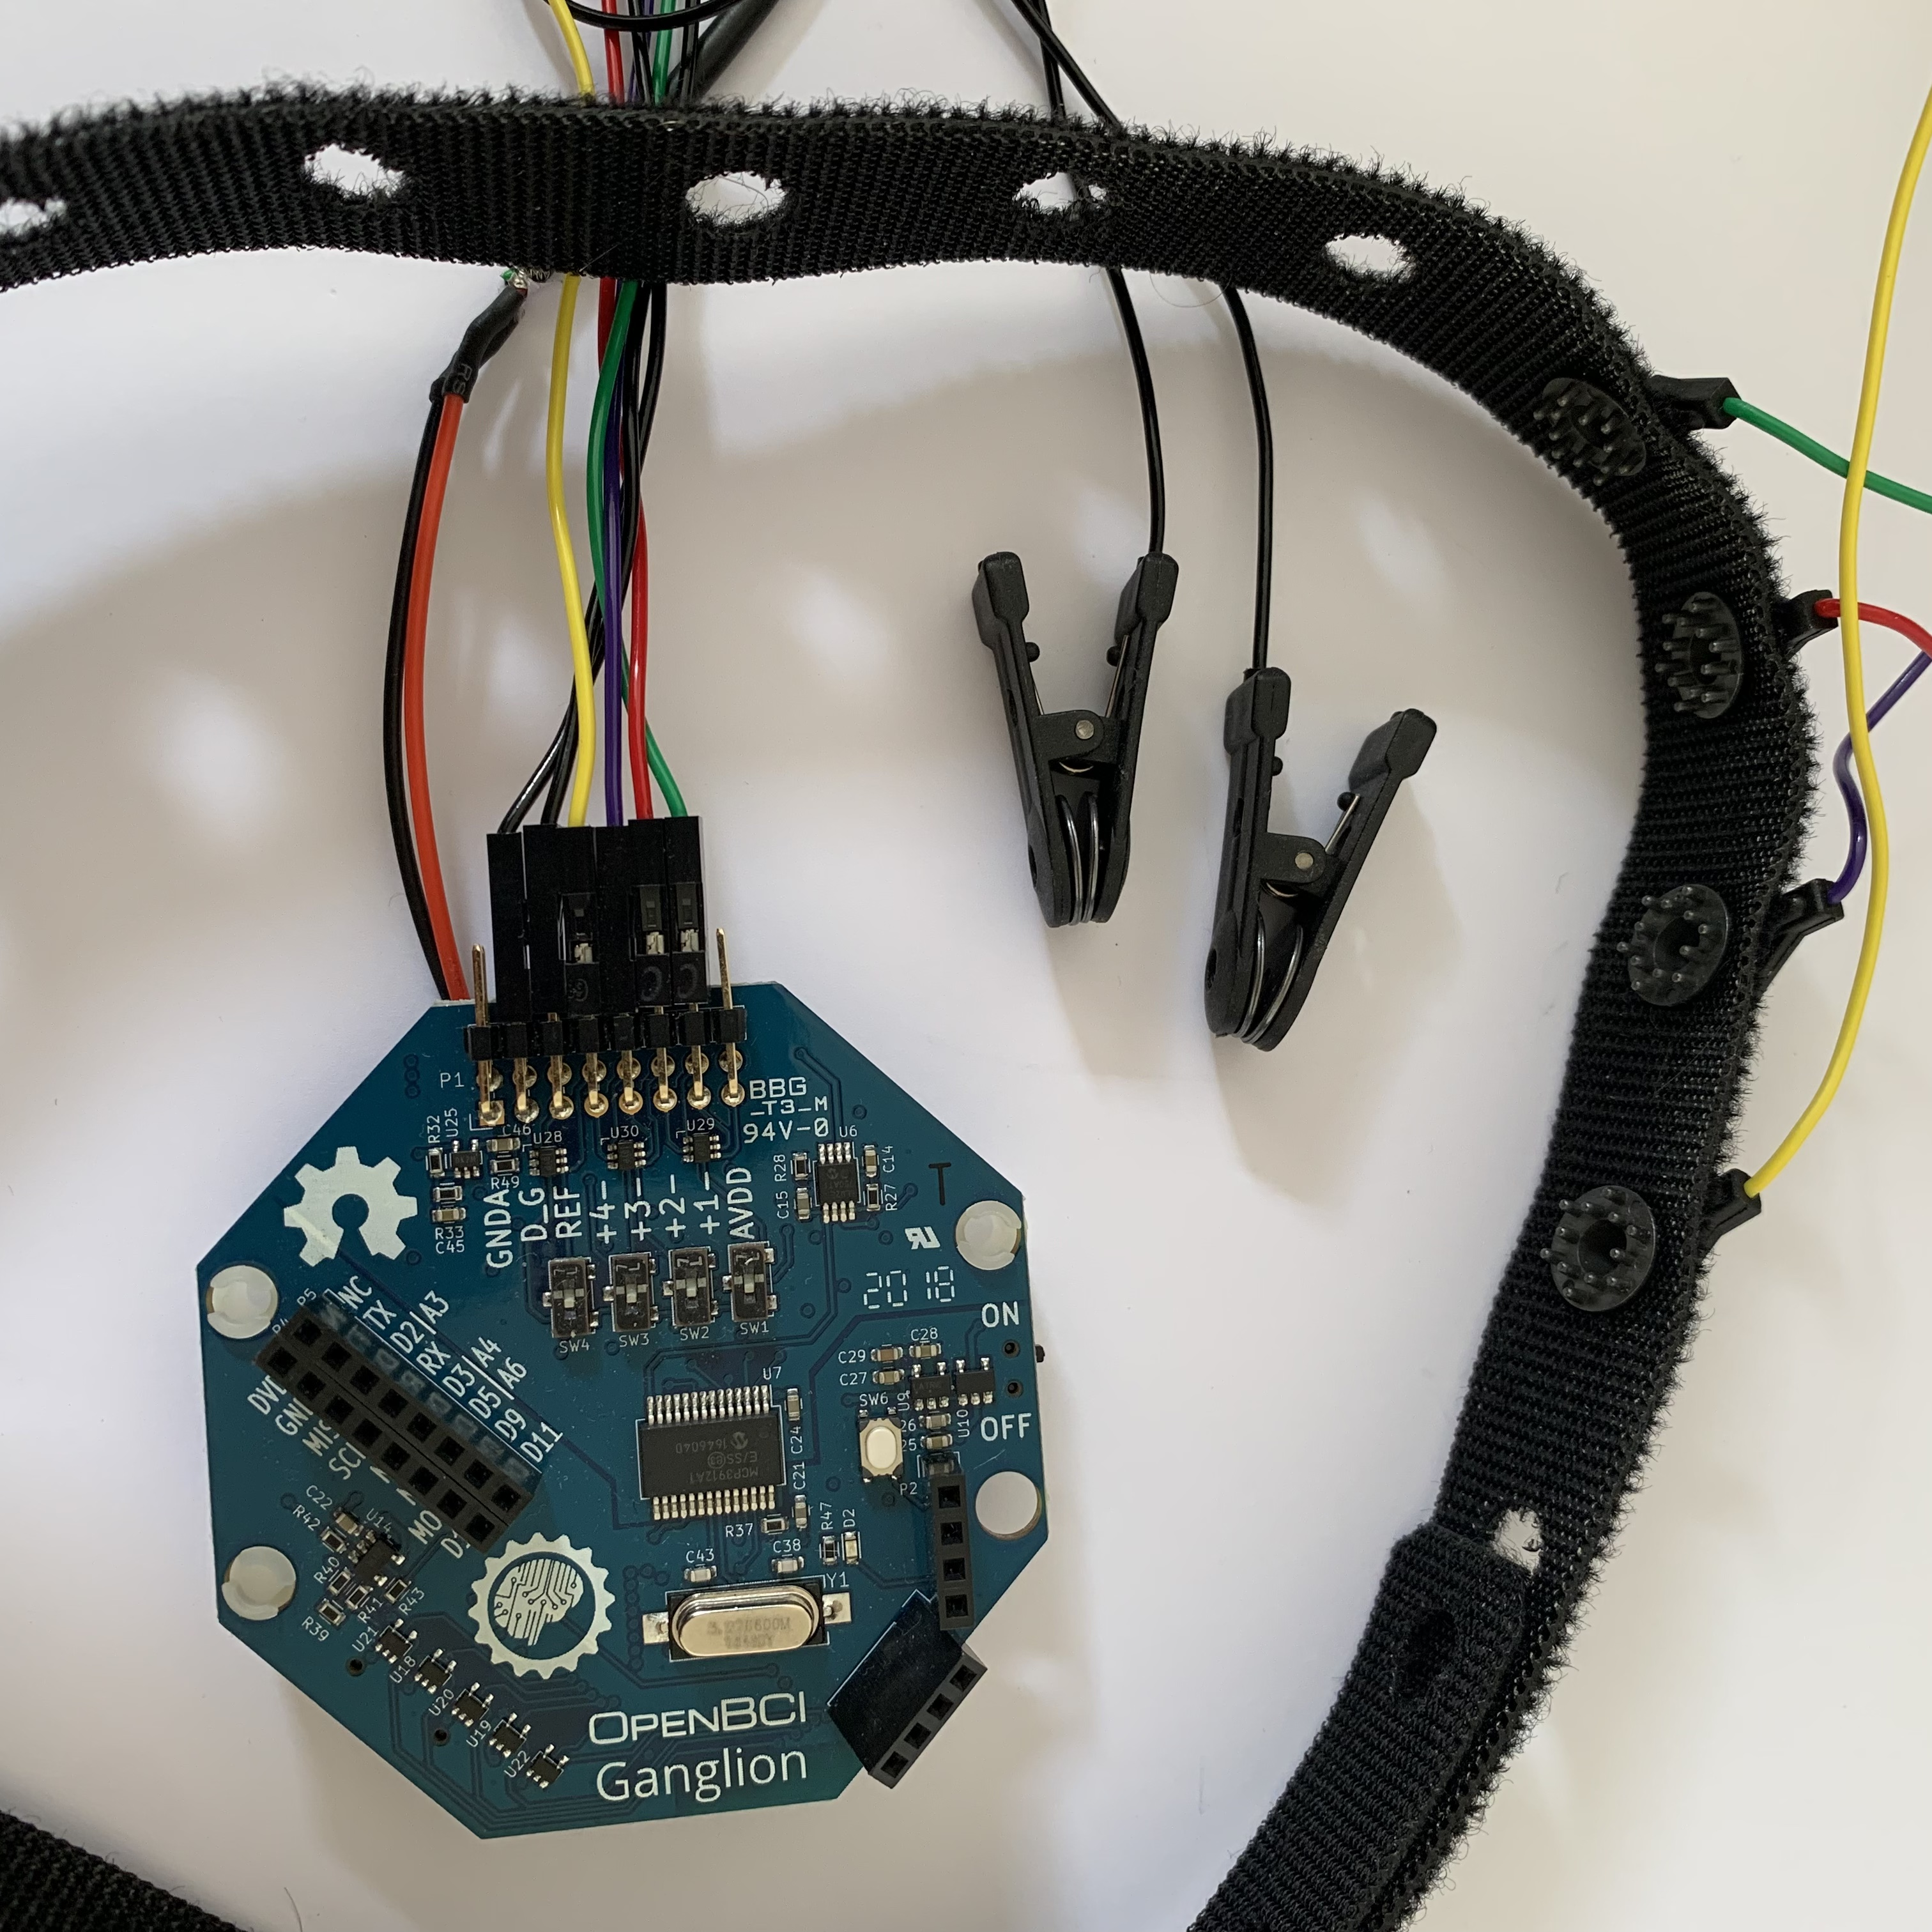
\includegraphics[width=\textwidth]{openbci}
         \caption{OpenBCI Ganglion board, electrodes and adjustable Velcro headband}
         \label{fig:openbci}
     \end{subfigure}
     \hfill
    \begin{subfigure}[c]{0.45\textwidth}
         \centering
         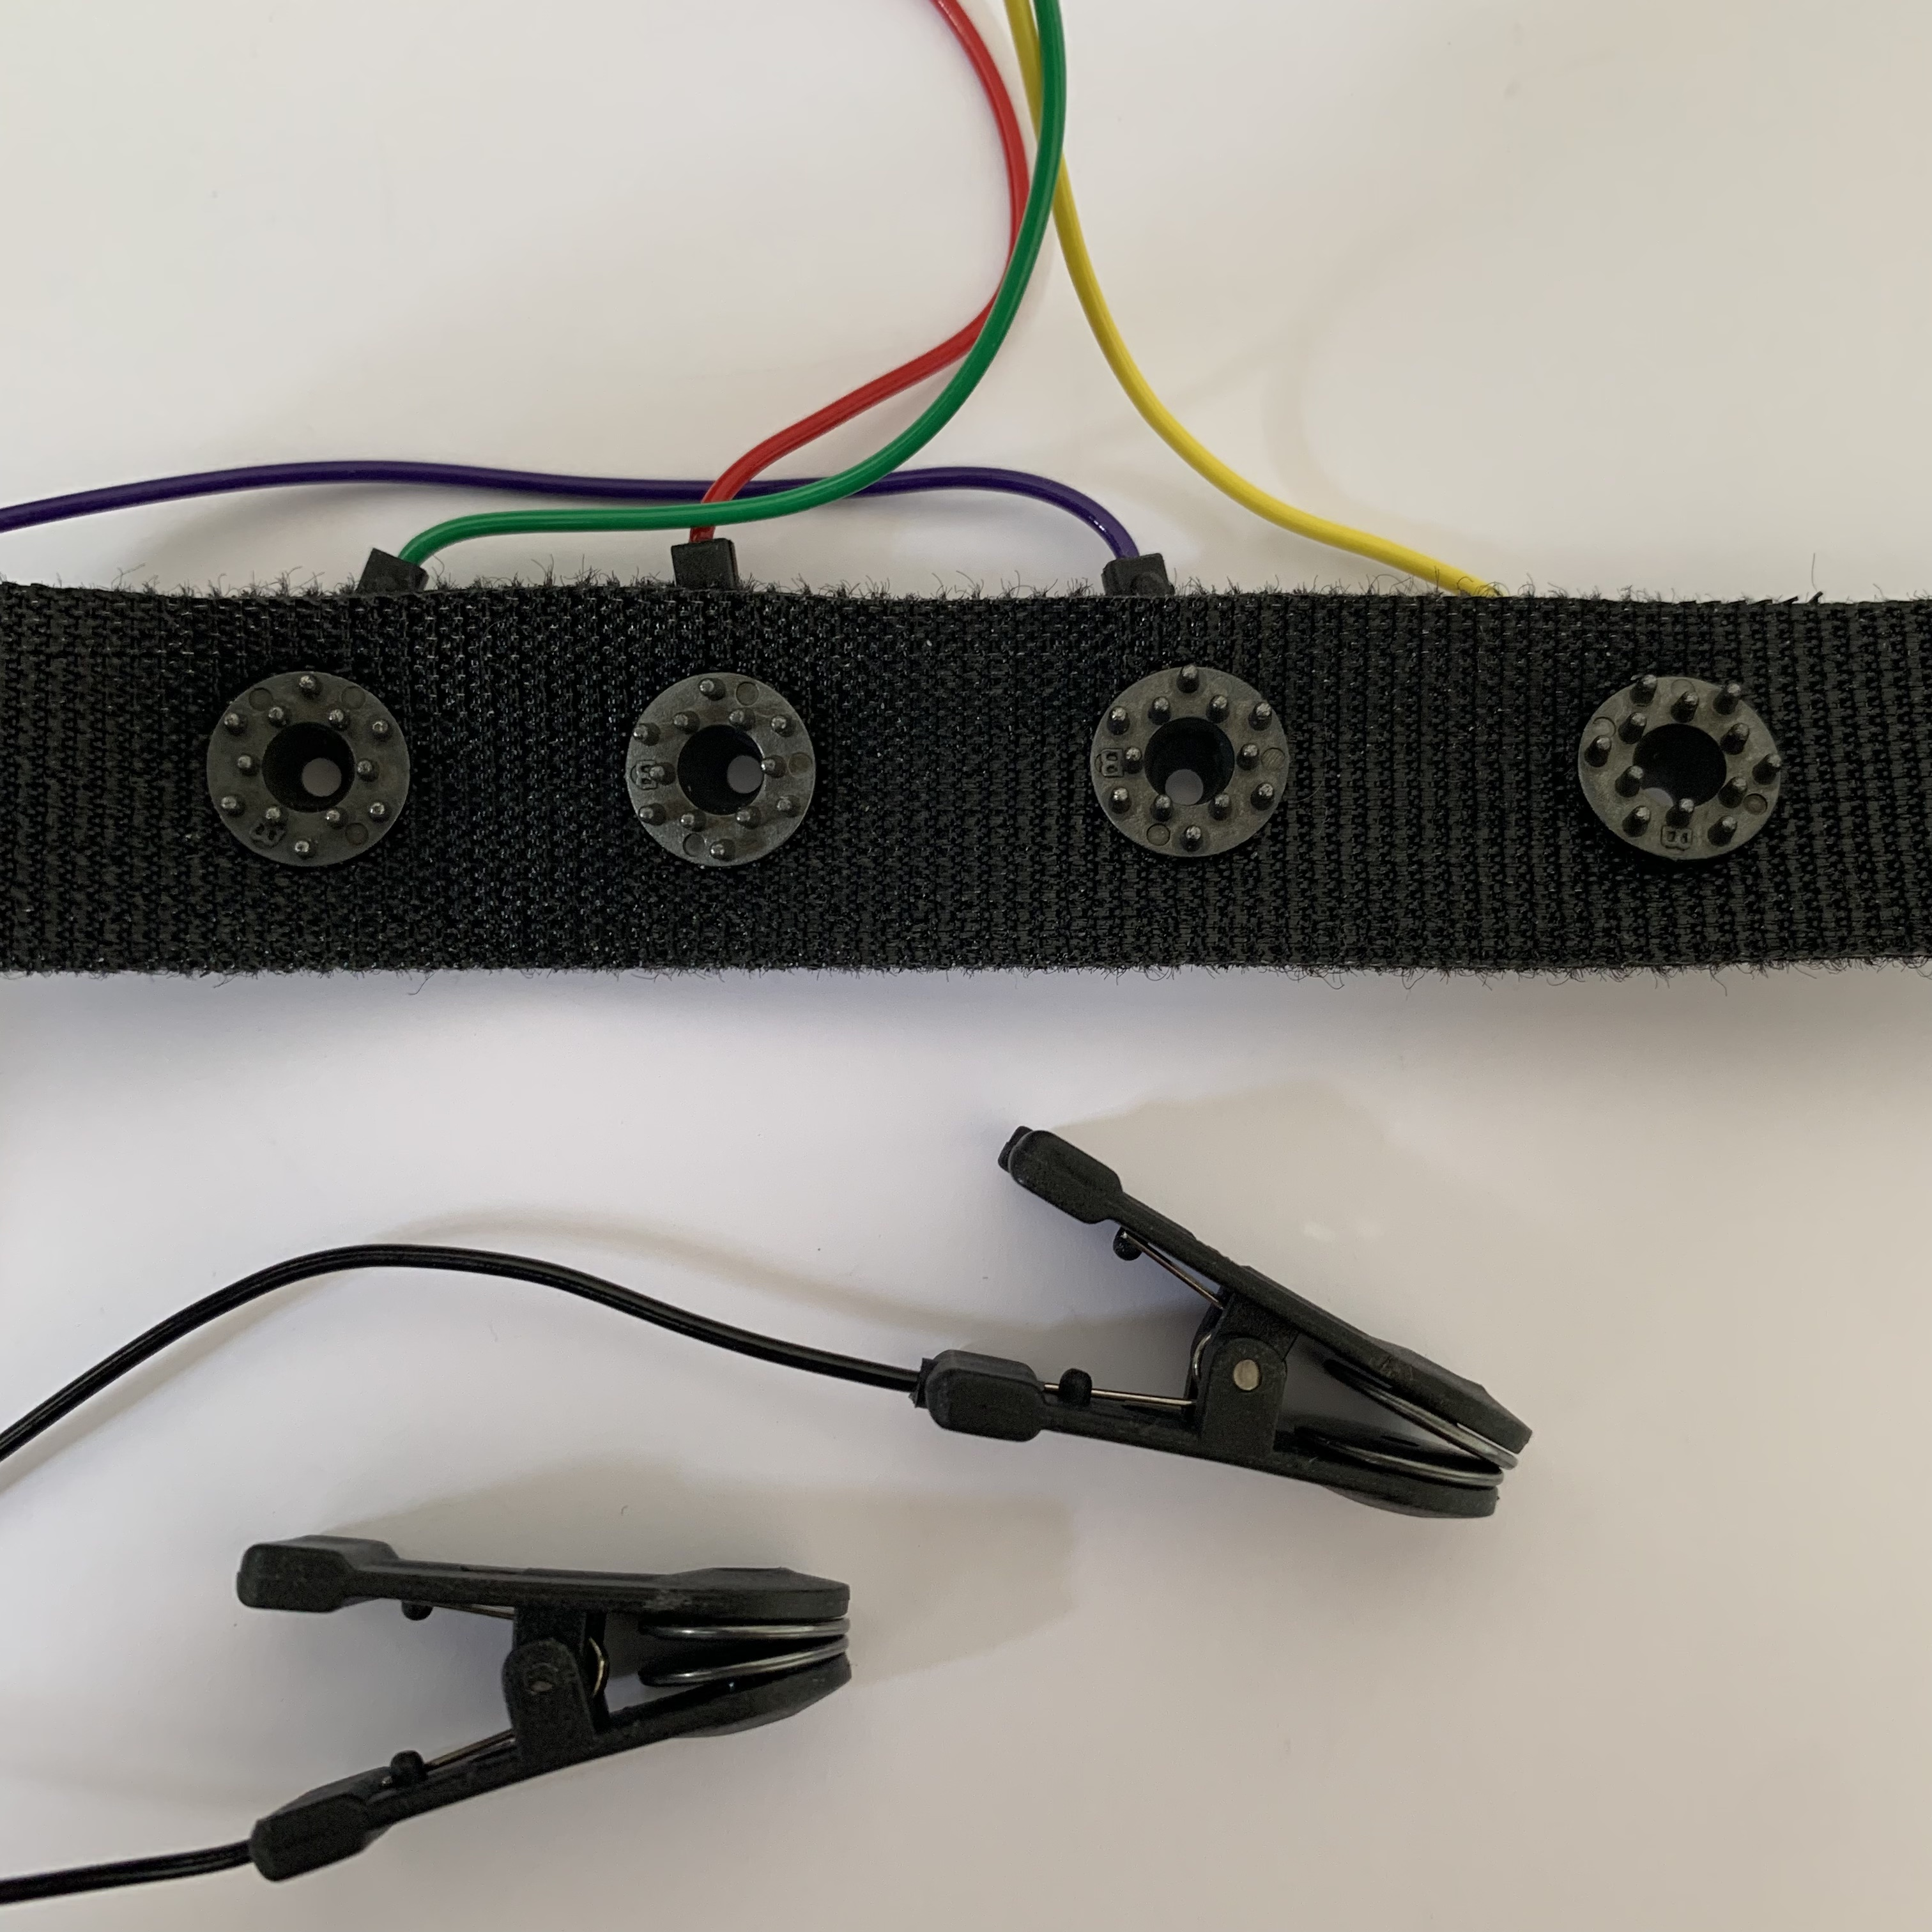
\includegraphics[width=\textwidth]{openbci-electrodes}
         \caption{Close-up view of the 4 active electrodes and two reference electrode clips (bottom)}
         \label{fig:openbci-electrodes}
     \end{subfigure}
        \caption[Images of the OpenBCI Ganglion bio-sensing device and electrodes]{Images of the OpenBCI Ganglion bio-sensing device and electrodes. The two black clips are the reference electrodes and the four active channels are received through the coloured wires.}
        \label{fig:openbci-subfigs}
\end{figure}
As depicted in Figure \ref{fig:openbci-subfigs}, the Ganglion board offers four active channels. All four channels were using during experimentation as it was more convenient to exclude data from certain channels in post-processing than only measuring a subset of channels. Although wet electrodes can also be used with this kit, in accordance with the project constraints mentioned in Chapter \ref{chapter:introduction}, dry electrodes were used. As seen in Figure \ref{fig:openbci}, the four active electrodes have spiky nodules to increase surface pressure and thus improve contact quality with the scalp. For reference and comparison, some core features of the Ganglion board are provided below:
\begin{itemize}
    \item Microchip MCP3912 four channel 24-bit Delta-Sigma analogue frontend
    \item 200Hz sampling rate
    \item Simblee Bluetooth 4.0 module
\end{itemize}

\subsection{NGNI Prototype I}
\label{subsection:electronic-hardware-proto}
As alluded to in Chapter \ref{chapter:introduction}, the hardware to be used in this project was supplied by the Imperial NGNI Lab. All hardware prototypes developed by the Lab were based on the Espressif ESP32; a low-cost, low-power SoC (system-on-chip) based on the Tensilica Xtensa LX6 microprocessor with integrated Wi-Fi and Bluetooth. Features of the ESP32 that are relevant to this project include \cite{esp32-digikey}:
\begin{itemize}
    \item dual-core, 240MHz CPU
    \item onboard FPU
    \item 12-bit successive-approximation (SAR) ADC
    \item 4x SPI, 2x I2C, 3x UART interfaces
    \item up to 600 DMIPS performance
    \item ultra low-power (ULP) co-processor
    \item 4 MiB SRAM
    \item integrated Wi-Fi 802.11 b/g/n and BLE
\end{itemize}
The ESP32 is extremely capable for its low price tag of around 3.6 USD \cite{esp32-digikey}. Its dual-core CPU is also particularly attractive as it could allow decoding-related computation and network communication to happen concurrently.

Figure \ref{fig:esp-hardware} shows the electronic hardware prototype developed by the NGNI Lab. In this design, the active components directly involved in the normal functioning of the system are independently located on a `target' board. A second programmer board was created to enable serial communication with the target; most commonly in order to flash new firmware to it during development. The programmer board uses six spring-loaded pogo pins to make momentary contact with corresponding pads on the target board during development. These 6 pins, and their corresponding pads on the target board, can be seen directly in the centre of Figure \ref{fig:esp-hardware-both}. A 3D printed housing was created to facilitate correct contact between the boards during development. As depicted in the image of the programmer board in Figure \ref{fig:esp-hardware-programmer}, it also features contact points for probing a few selected pins/junctions on the target board such as: the ADC output, the output of the instrumentation amplifier, the output of the analogue filter and all relevant supply voltage references. In addition, two momentary push-buttons connected to the \texttt{BOOT0} and \texttt{EN} pins of the ESP32 SoC are included in order to allow hardware resets and to control the entry state upon reset: bootloader mode or normal operating mode. 

\begin{figure}[!htb]
     \centering
     \begin{subfigure}[b]{0.3\textwidth}
         \centering
         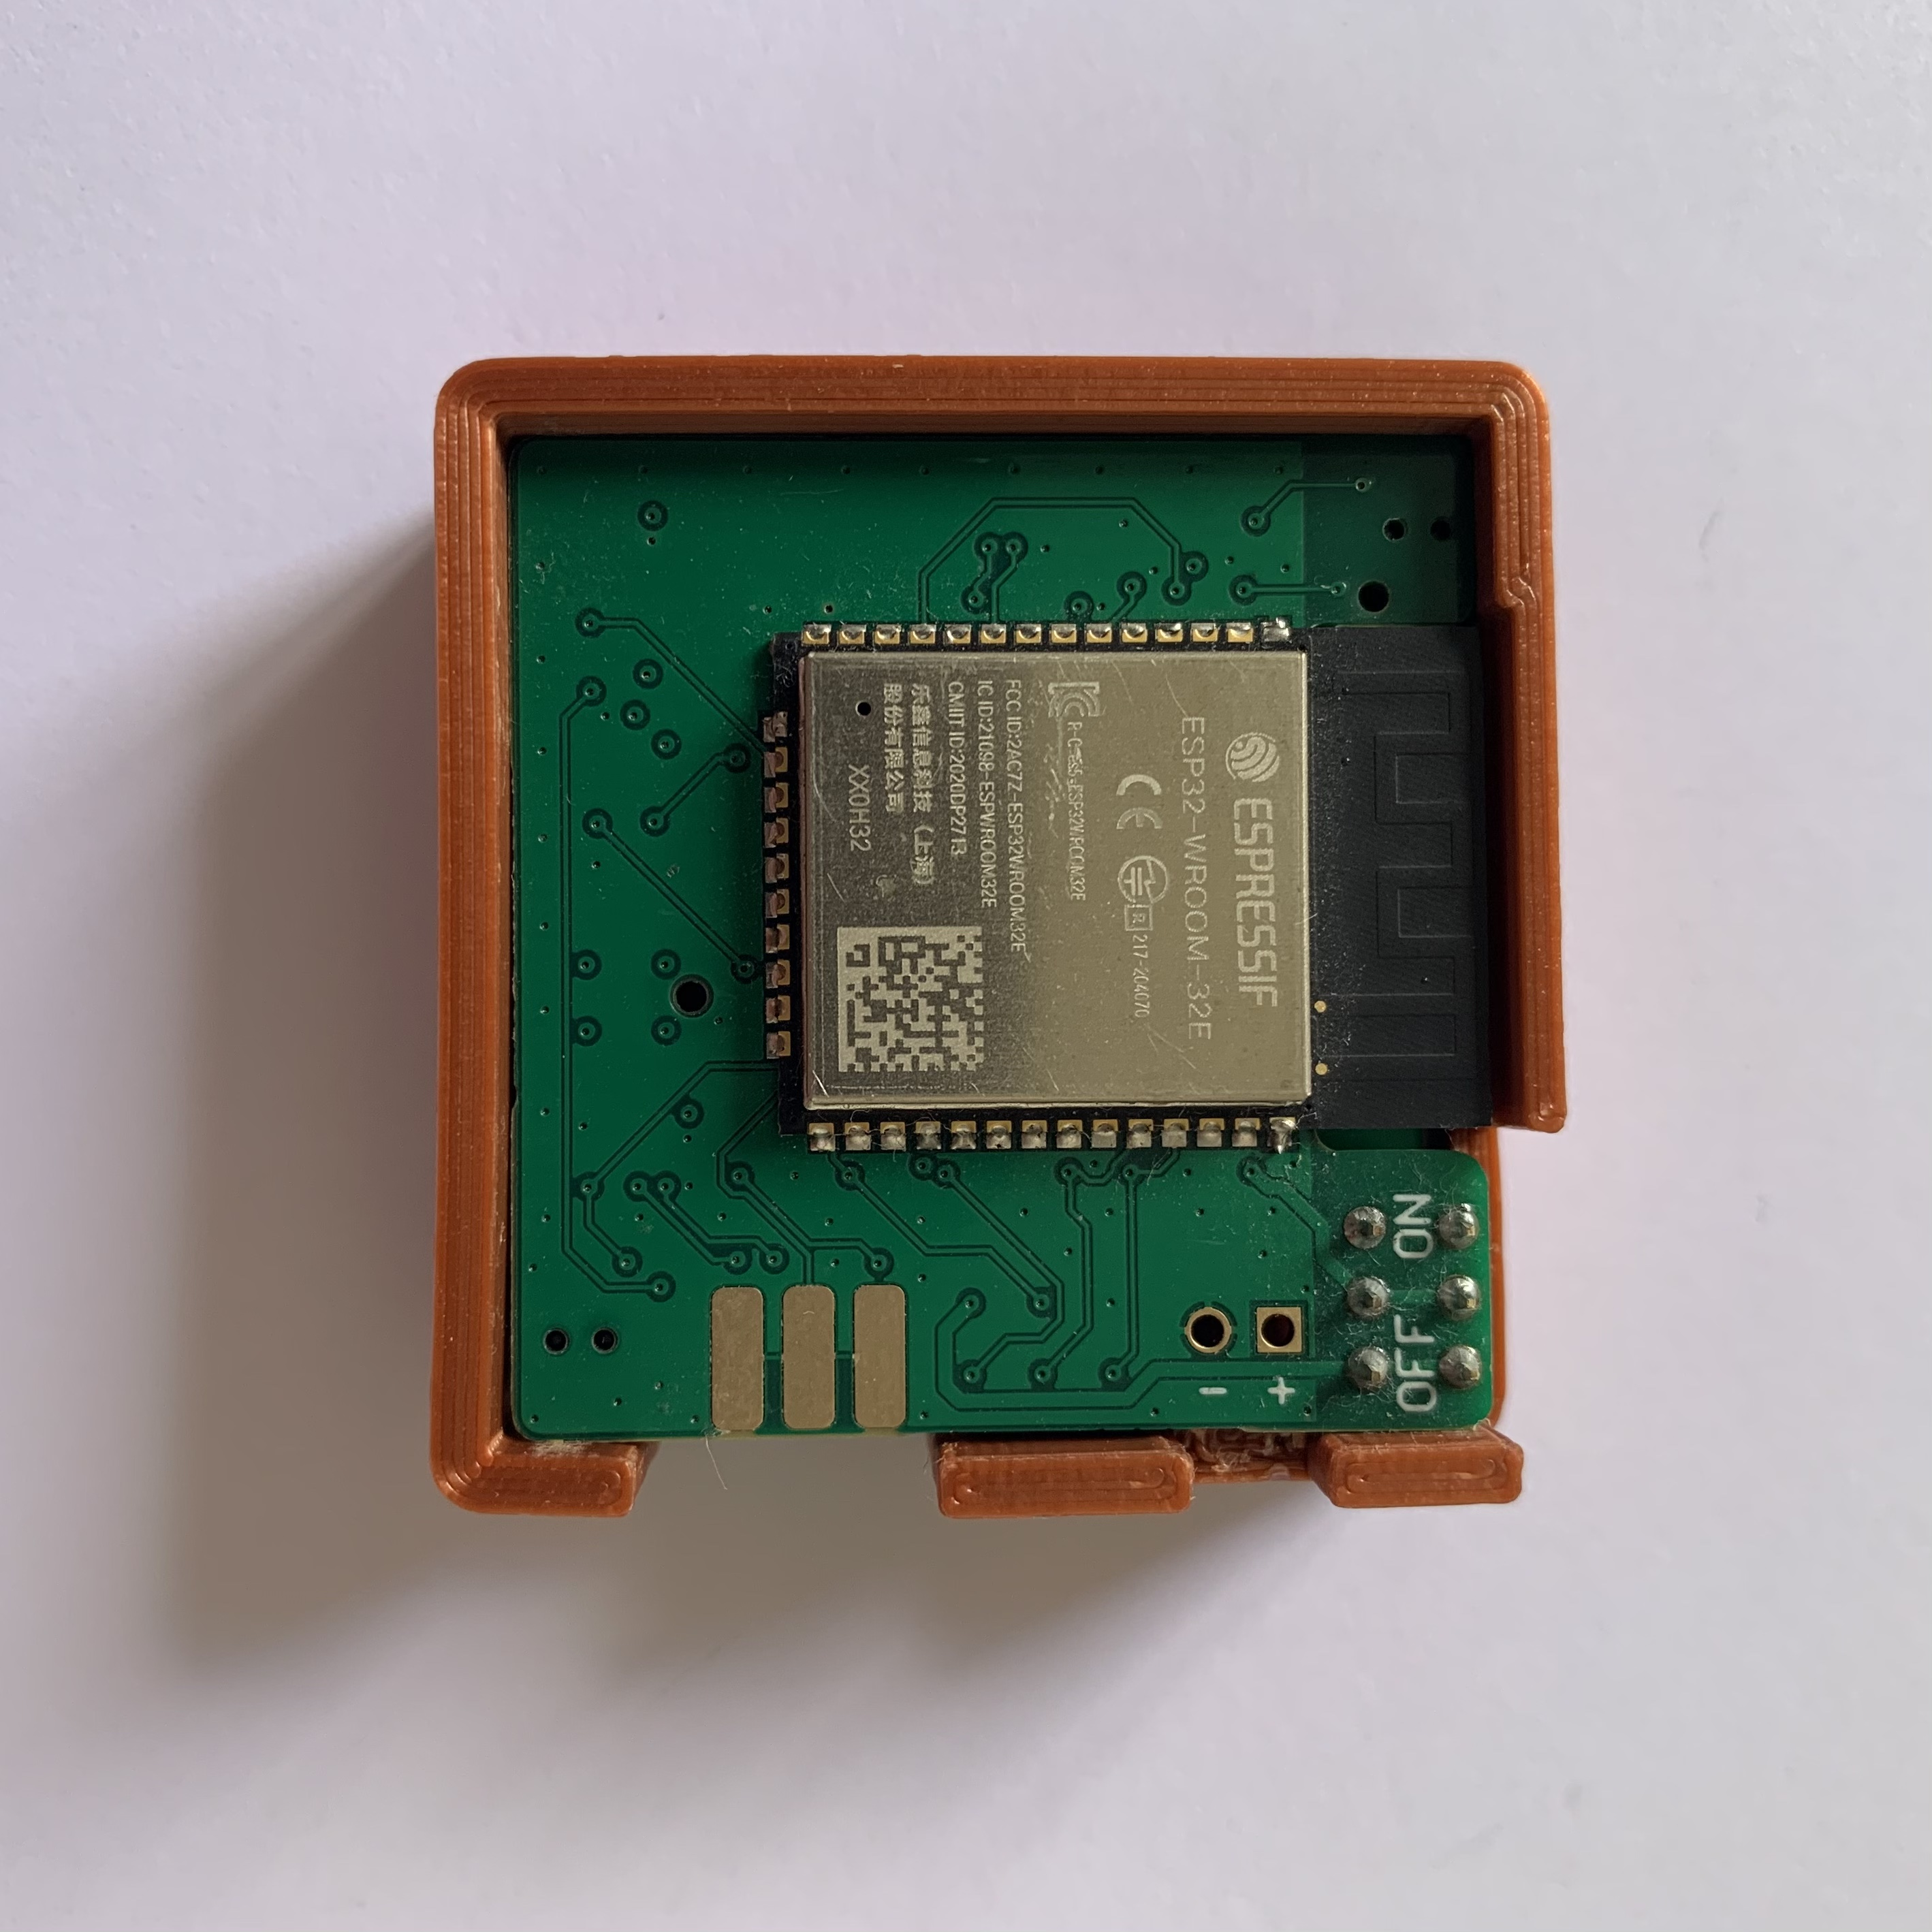
\includegraphics[width=\textwidth]{esp-top}
         \caption{Target board with ESP32 SoC and peripheral electronics}
         \label{fig:esp-hardware-soc}
     \end{subfigure}
     \hfill
     \begin{subfigure}[b]{0.3\textwidth}
         \centering
         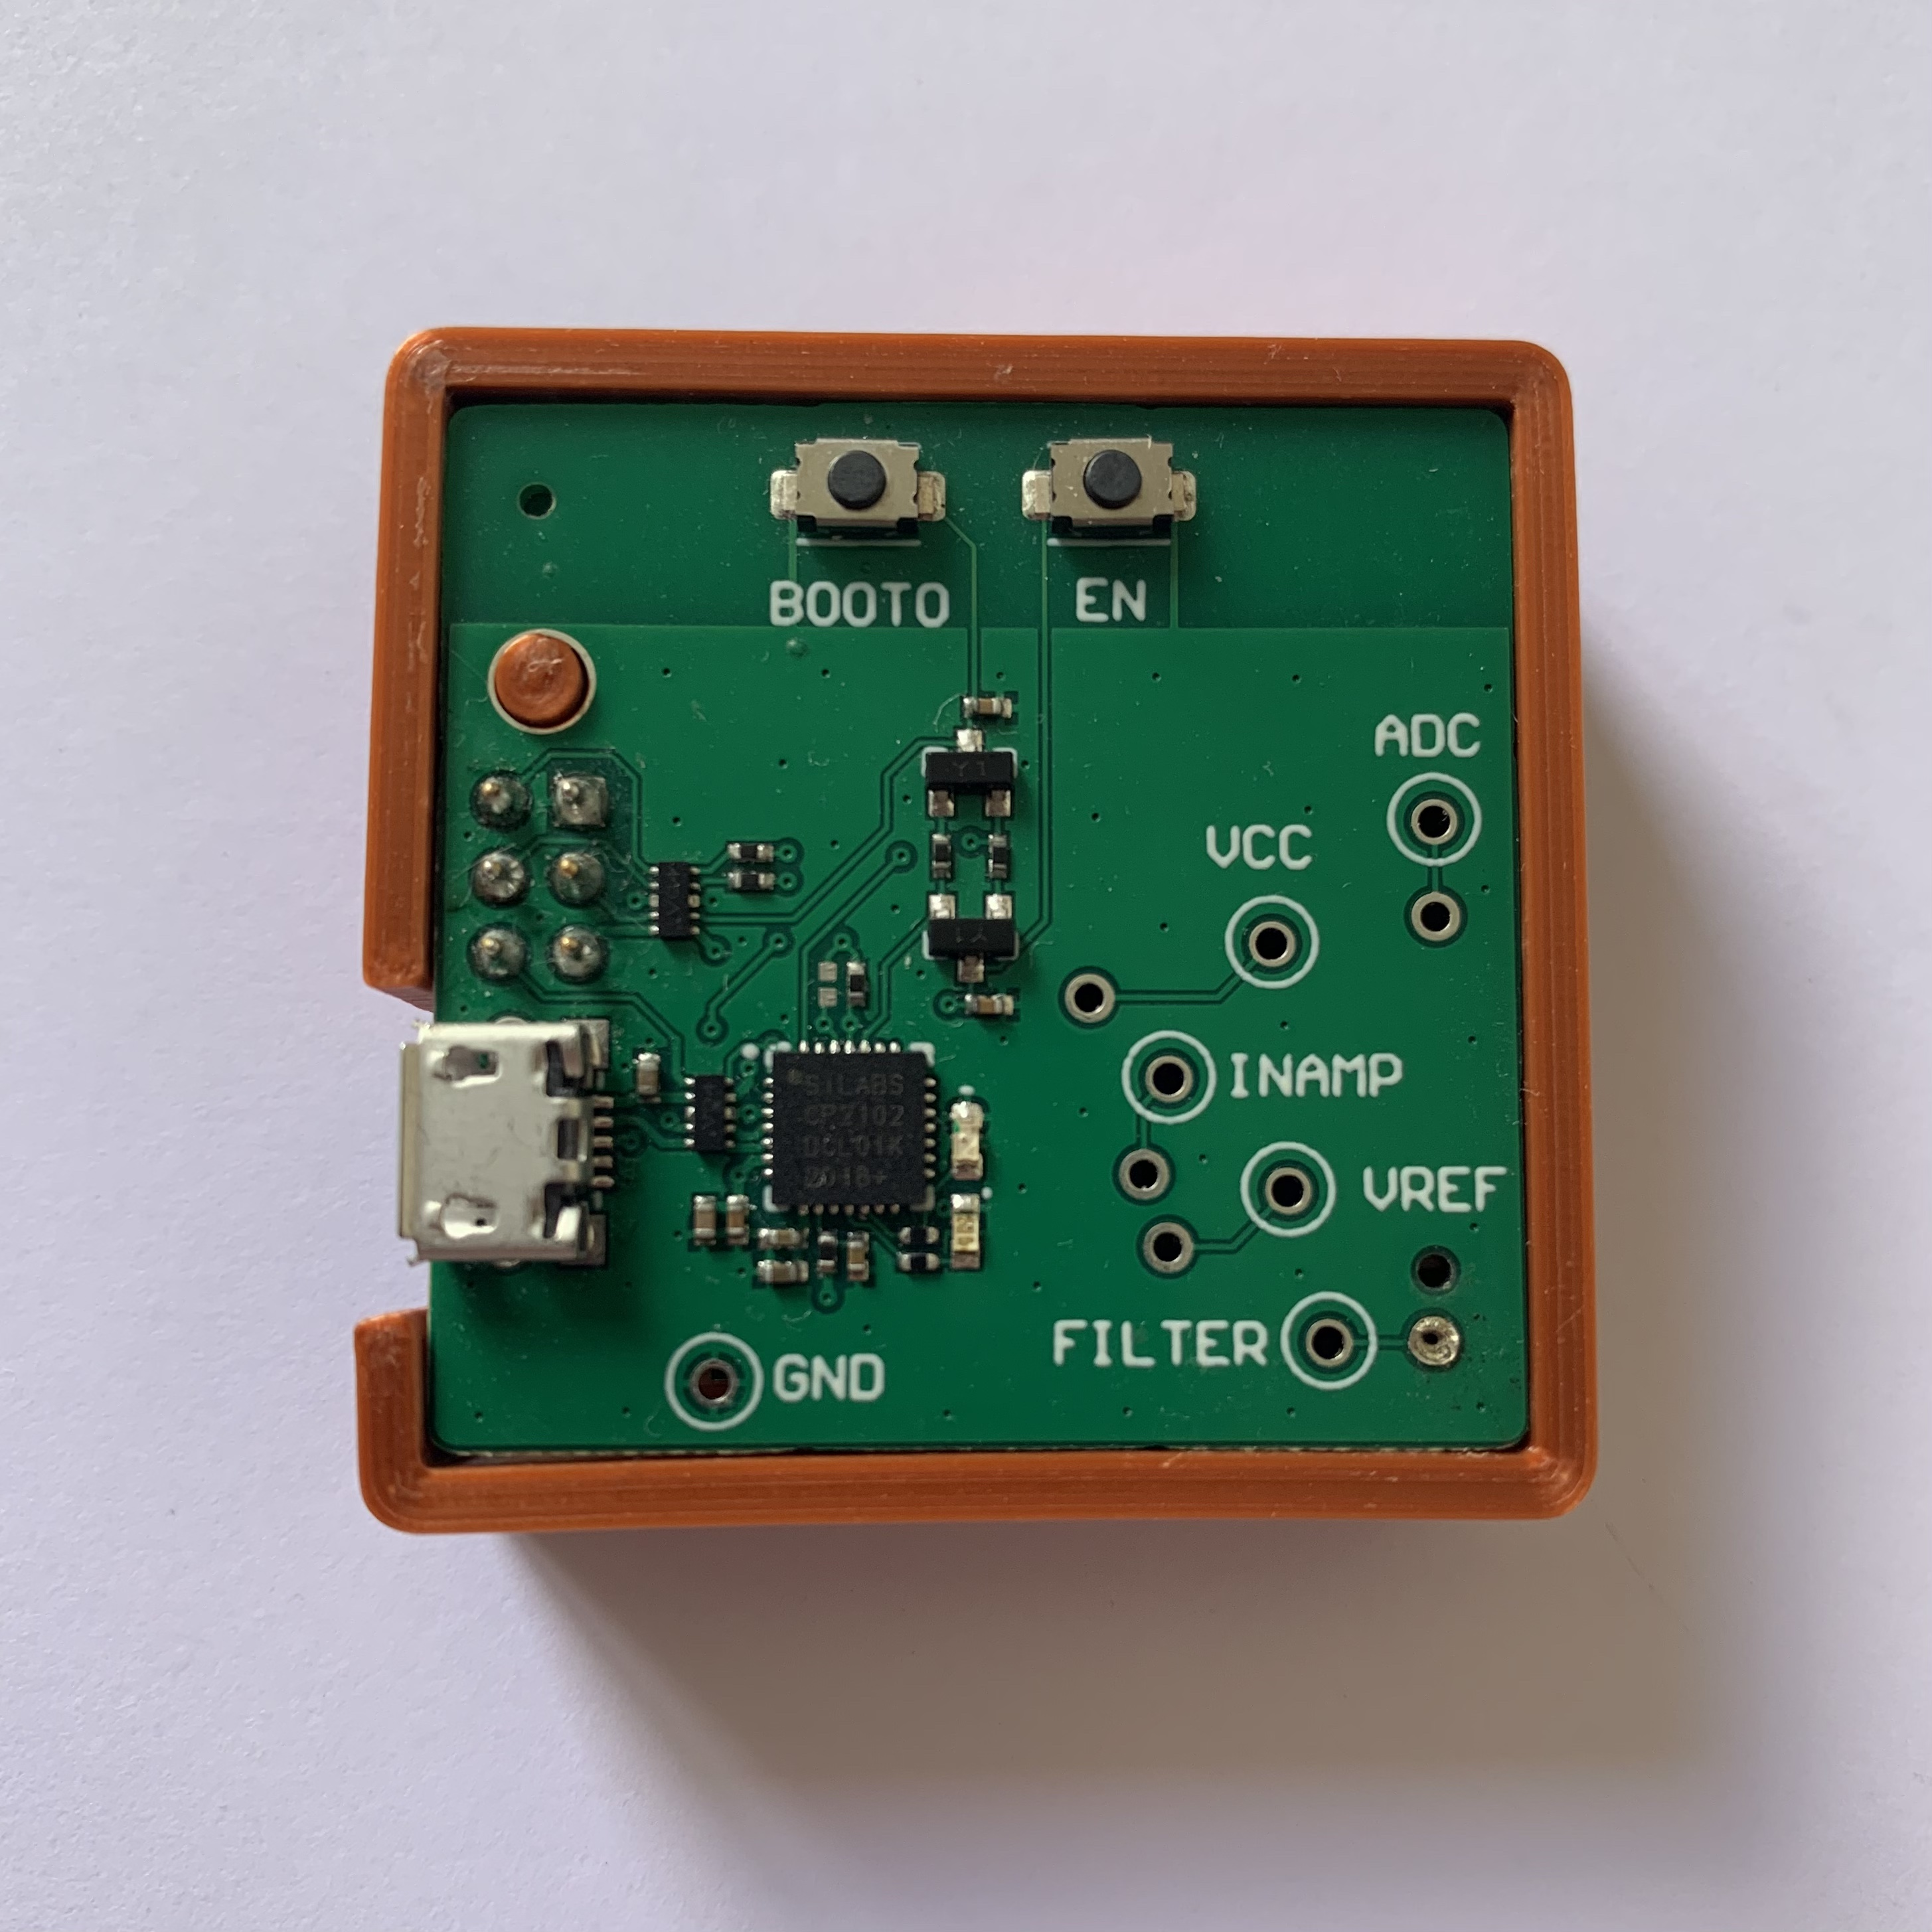
\includegraphics[width=\textwidth]{programmer}
         \caption{Programmer board with serial-to-USB interface }
         \label{fig:esp-hardware-programmer}
     \end{subfigure}
     \hfill
    \begin{subfigure}[b]{0.3\textwidth}
         \centering
         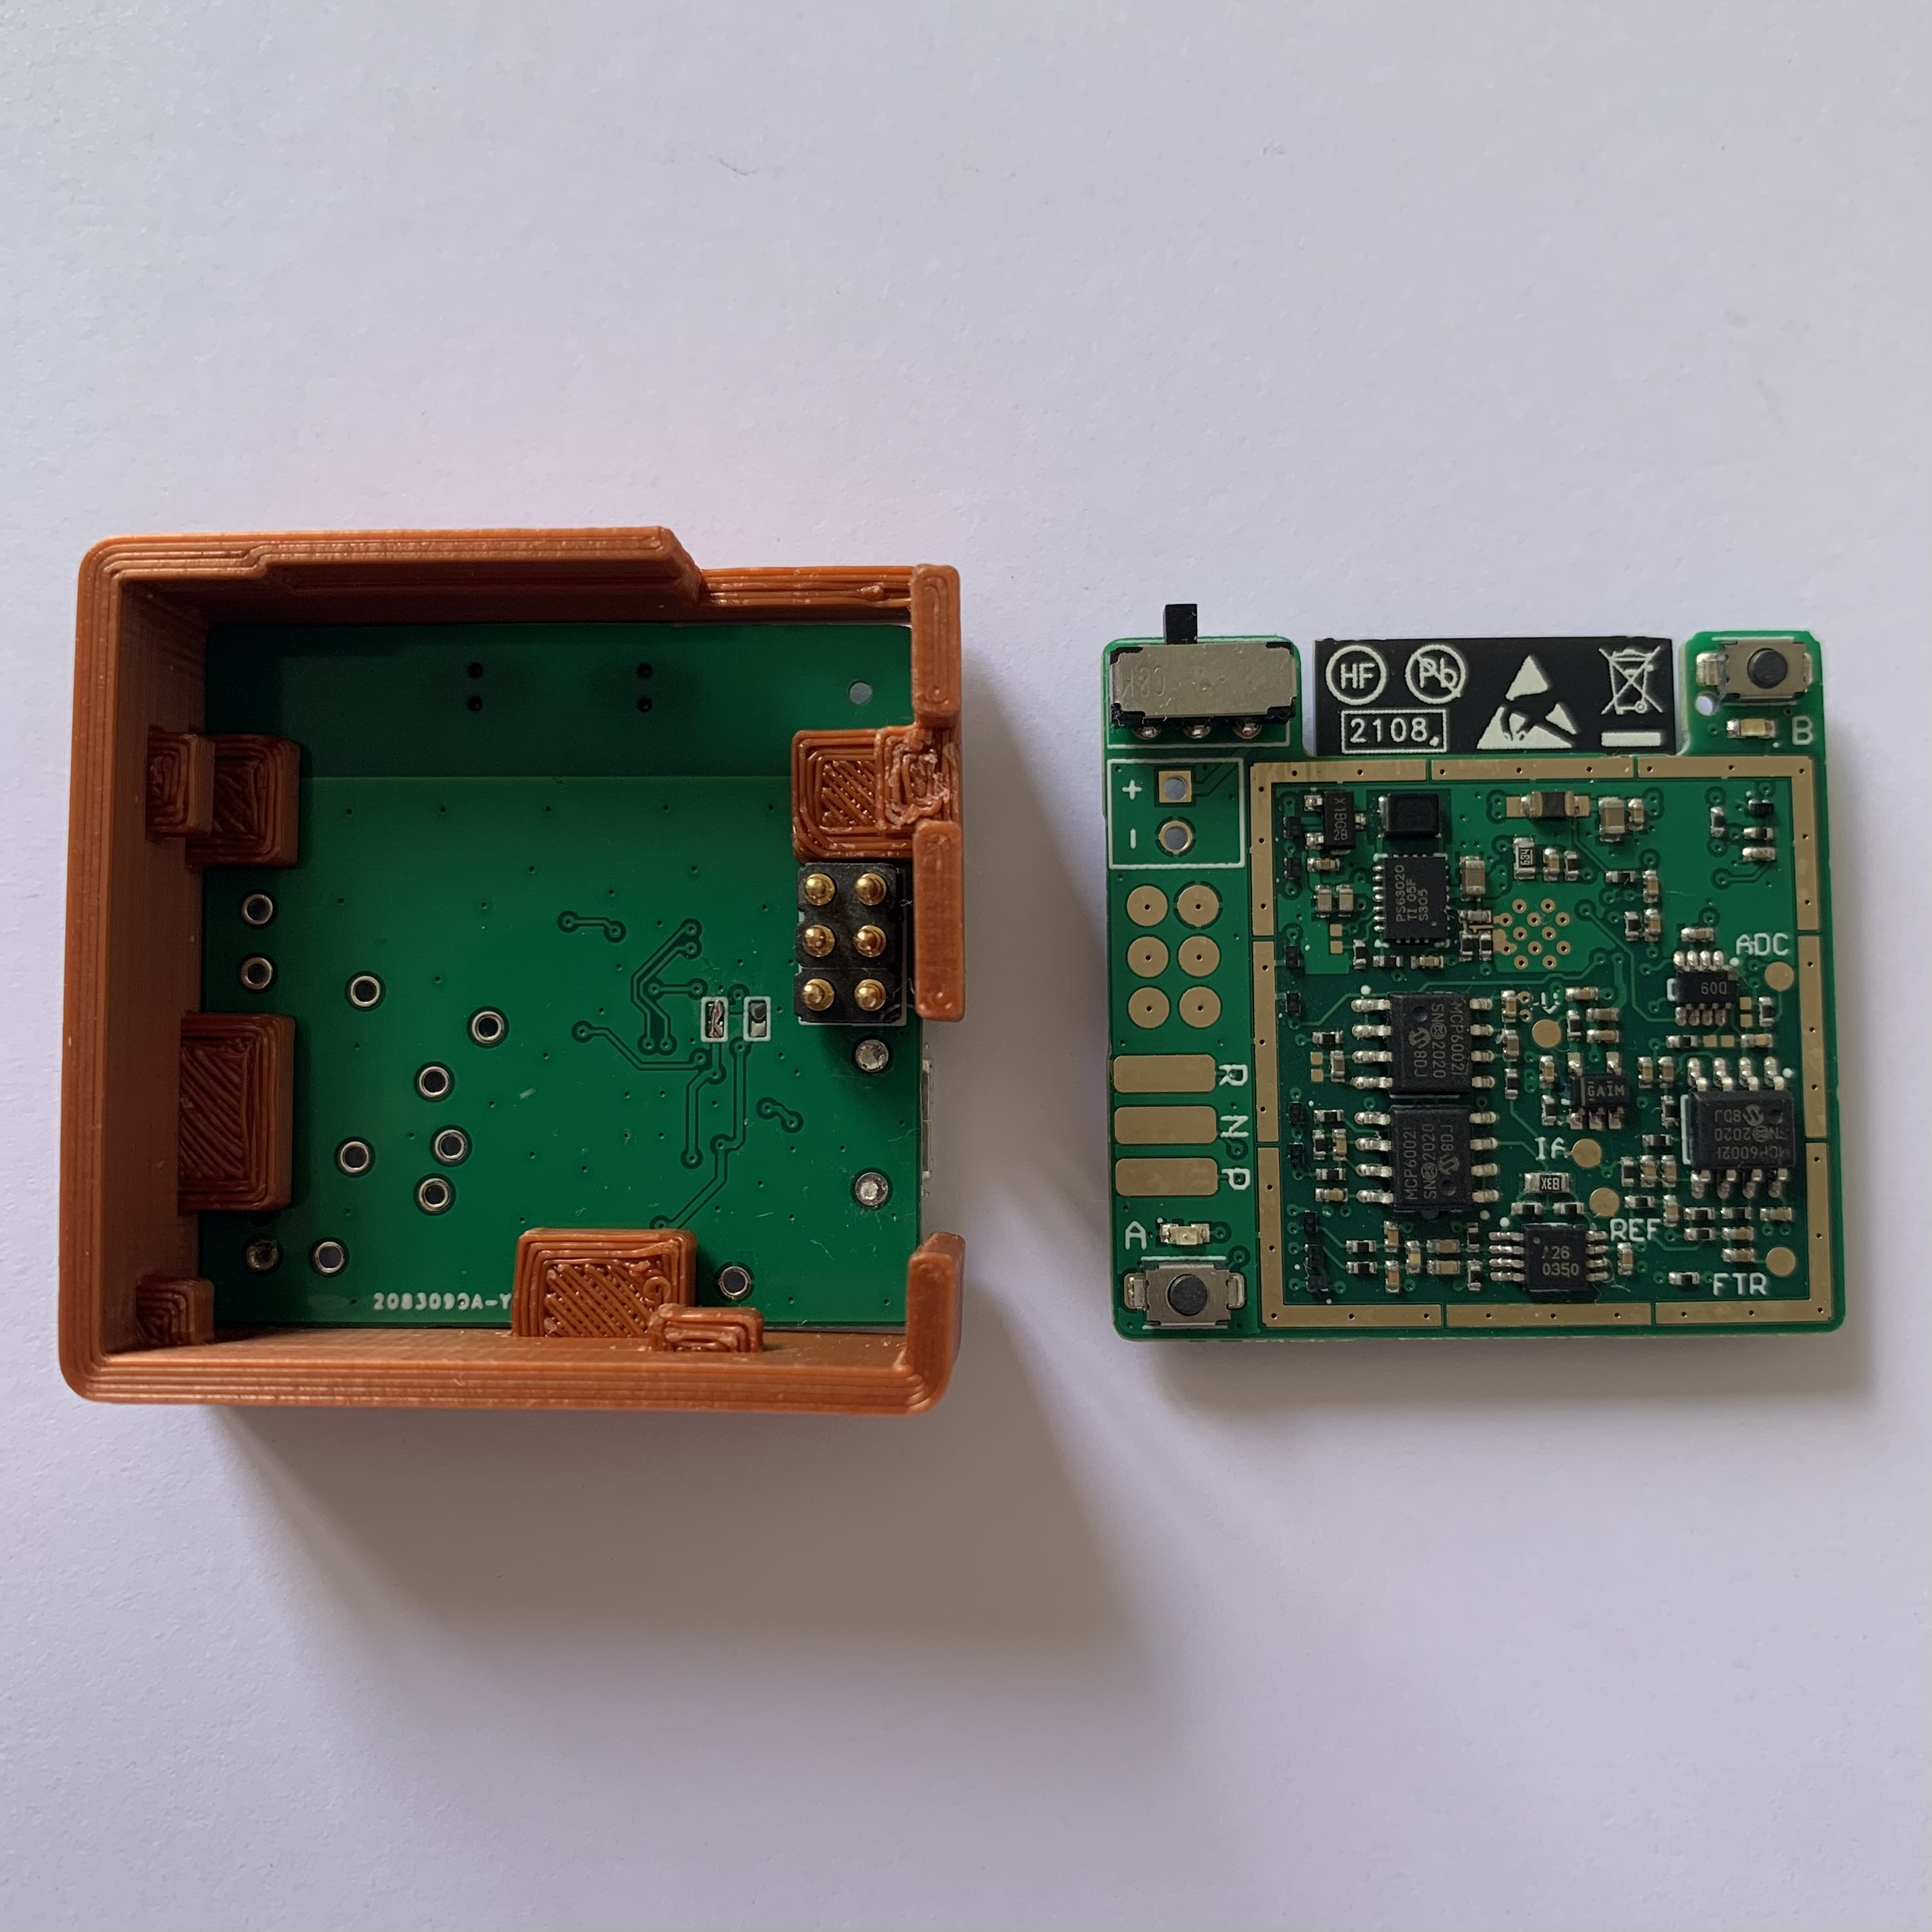
\includegraphics[width=\textwidth]{esp-both}
         \caption{Bottom side of the programmer board (left) and target board}
         \label{fig:esp-hardware-both}
     \end{subfigure}
        \caption[Images of the electronic hardware prototype developed in the Imperial NGNI Lab]{Images of the electronic hardware prototype developed in the Imperial NGNI Lab. This prototype includes the target board with ESP32 SoC, as well as a programmer board that is used to flash new firmware on to the microcontroller aboard the target board. The orange 3D-printed housing is used to position the programmer board above the target during firmware updates or other serial communication with an external computer.}
        \label{fig:esp-hardware}
\end{figure}

\subsubsection{Analogue signal processing system}

Figure \ref{fig:analogue-system-c4} provides an overview of the key analogue signal processing elements in the electronic hardware prototype. This system is primarily responsible for amplifying $\mu$V-scale raw EEG signals, filtering out 50Hz mains power interference and offering further amplification that can be adjusted in firmware. 

\begin{figure}
    \centering
    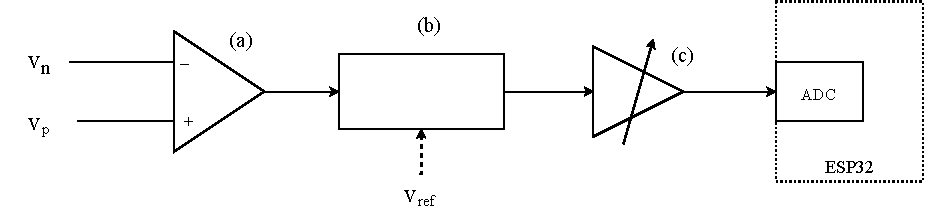
\includegraphics[width=\textwidth]{analogue-system}
    \caption[Functional overview diagram of the analogue signal processing system in the NGNI electronic hardware prototype.]{Functional overview diagram of the analogue signal processing system in the NGNI electronic hardware prototype. (a) signals captured from the two active electrodes, $\textrm{v}_n$ and $\textrm{v}_p$, first pass through a differential instrumentation amplifier. (b) a third order hour glass low-pass filter is used for 50Hz mains power rejection. (c) the filtered signal can be further amplified with adjustable gain that is controlled via a digital potentiometer through a SPI interface.}
    \label{fig:analogue-system-c4}
\end{figure}

Important details of the components shown in Figure \ref{fig:analogue-system-c4} are provided below:

\begin{enumerate}[label=(\alph*)] % (a), (b), (c), ...
\item differential instrumentation amplifier
\begin{itemize}
    \item fixed gain of 1120
    \item high-pass filter dynamics: highest corner frequency $f_c=0.48$Hz
\end{itemize}
\item hourglass low-pass filter
\begin{itemize}
    \item Q factor 2.17
    \item low-pass corner frequency $f_c=37.4$Hz
    \item notch frequency $f_n=50$Hz
    \item 50Hz rejection characteristics: minimum 17dB, nominal 35dB and maximum 55dB.
\end{itemize}

\item adjustable-gain output amplifier
\begin{itemize}
    \item adjustable gain between 1.745 and 19.2
    \item input low-pass filter dynamics: corner frequency of $f_c=36.35$Hz 
\end{itemize}
\end{enumerate}
Important to note is that the analogue hourglass filter designed for 50Hz rejection has a corner frequency of $f_c=37.4$Hz. Therefore, EEG signals with harmonics beyond $37.4$Hz will start to become attenuated as a side-effect of the dynamics of this filter. Furthermore, as mentioned in Section \ref{subsection:nature-of-eeg-signals}, raw EEG signals are expected to be in the range of 0.5 to 100$\mu$V peak-to-peak. Neglecting other minor sources of gain or attenuation in the system, the ranges of signal amplitudes (peak-to-peak voltages) at the output of the system for various input EEG signal amplitudes and gain configurations is shown in Table \ref{tab:gain-voltage-ranges}. Note that, with the minimum gain configuration of $g_2=1.745$ on the output amplifier, the maximum expected output voltage is only $v_{\textrm{out}}=0.132$V which is approximately equal to the full range of amplitudes expected with this configuration.

\begin{table}[]
\centering
\begin{tabular}{@{}lllll@{}}
\toprule
\textbf{$\mathbf{v_{\textrm{in}}}$} ($\mu$V) & \textbf{$\mathbf{g_1}$} & \textbf{$\mathbf{g_2}$} & \textbf{$\mathbf{g_1g_2}$} & \textbf{$\mathbf{v_{\textrm{out}}}$} ($\textrm{V}$)\\ \midrule
0.5          & 1120        & 1.745       & 1315.4          & \textbf{0.000658}        \\
0.5          & 1120        & 19.2        & 21504           & 0.0108          \\
100          & 1120        & 1.745       & 1315.4          & 0.132           \\
100          & 1120        & 19.2        & 21504           & \textbf{2.15}            \\ \bottomrule
\end{tabular}
\caption[Table showing the theoretical range of voltages measured at the ADC of the ESP32 for varying input signal magnitudes and gain configurations]{Table showing the theoretical range of voltages $v_{\textrm{out}}$ at the input to the ADC of the ESP32 (output of the analogue signal processing system) with varying input signal amplitude $v_{\textrm{in}}$ and gain configurations. Fixed gain $g_1$ is that of the input stage differential amplifier and $g_2$ is the adjustable gain of the output amplifier. The expected EEG signal amplitude range, $v_{\textrm{in}}$, is from \cite{teplan-eeg-measurement}. Voltages shown are peak-to-peak amplitudes.}
\label{tab:gain-voltage-ranges}
\end{table}

It should be noted that this first revision of the electronic hardware prototype is designed for coupling with \textit{two} active electrodes but only allows for \textit{differential} signal measurements between these electrodes. Consequently, only a single `channel' is recorded by the ADC in the ESP32. A third reference electrode is also expected in order to offer a common voltage reference point between the two active channels. 

\subsubsection{Mechanical hardware prototype}
\label{subsection:mech-hardware-frankenstein}
The very first complete EEG headband prototype comprising electronic and mechanical hardware is shown in Figure \ref{fig:frakenstein-hardware}. This version did not include any means of adjusting the circumference of the band of the electrode positions within it besides having to drill new holes in it. As such, this makeshift prototype was more intended to serve as a preliminary means of gathering real-life data using the electronic hardware. It was not designed (nor expected) to produce viable results for SSVEP decoding. 

\begin{figure}
    \centering
    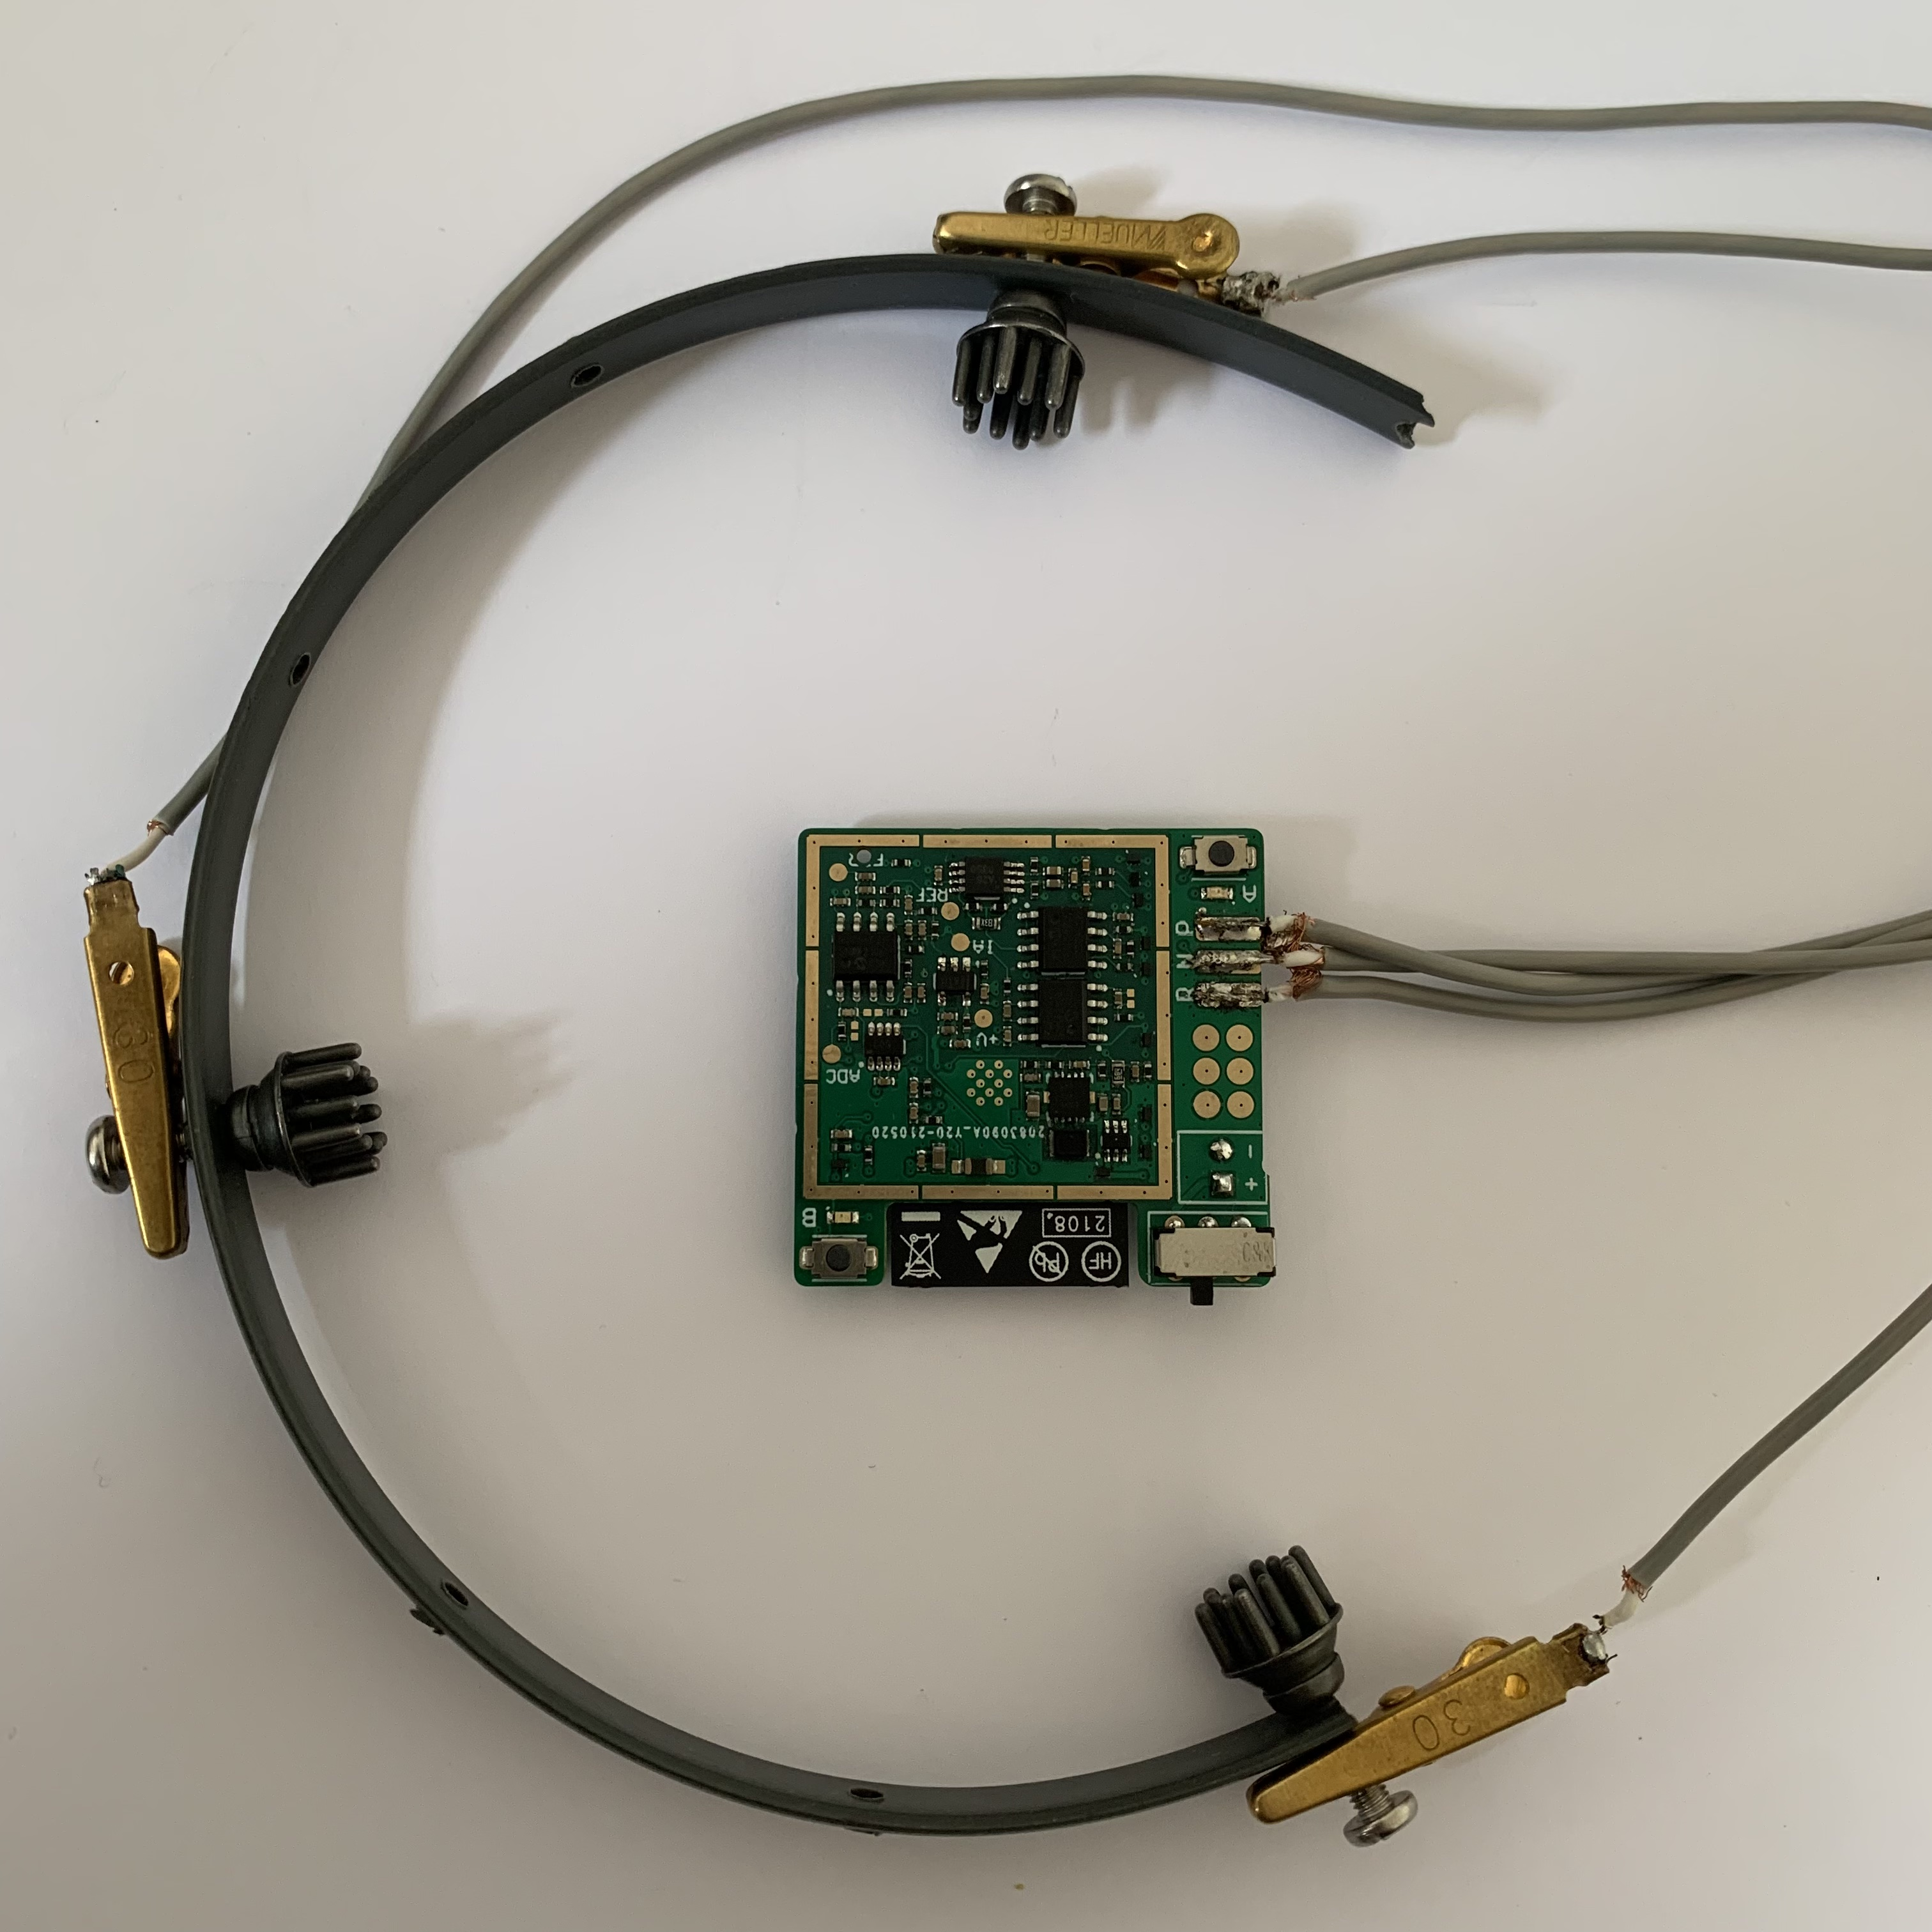
\includegraphics[width=0.6\textwidth]{frankenstein}
    \caption[A very rudimentary first prototype EEG headband]{The first very rudimentary prototype EEG band developed by the NGNI Lab based on the electronic hardware prototype in Figure \ref{fig:esp-hardware}. The active electrodes are those at the two extremes of the band and the middle one is a reference electrode.}
    \label{fig:frakenstein-hardware}
\end{figure}

\subsection{NGNI Prototype II}
Guided by the first EEG headband prototype, a second, improved version was developed by the NGNI Lab. This version, pictured in Figure \ref{fig:final-headband-subfigs}, employed a flexible and adjustable strap mechanism. This enabled the band circumference to be adjusted so as to offer greater comfort for the user and ensure appropriate contact pressure with heads of any size or morphology. Furthermore, electrodes could be adjusted more easily thanks to the 3D-printed locator structures in which they were housed. These locator structures, seen in Figure \ref{fig:final-headband-electrodes}, allowed for greatly improved contact angles between the electrodes and the scalp surface compared to the first prototype. In particular, the slight pitch and yaw flexibility introduced by the electrode locators allowed the electrodes to remain perpendicular to the undulating scalp surface, thereby maximising contact surface area. However, their stiffness also prevented excessive pitch and yaw deviations which may have arisen if the electrodes were housed directly in the flexible headband strap.

\begin{figure}
     \begin{subfigure}[c]{0.48\textwidth}
         \centering
         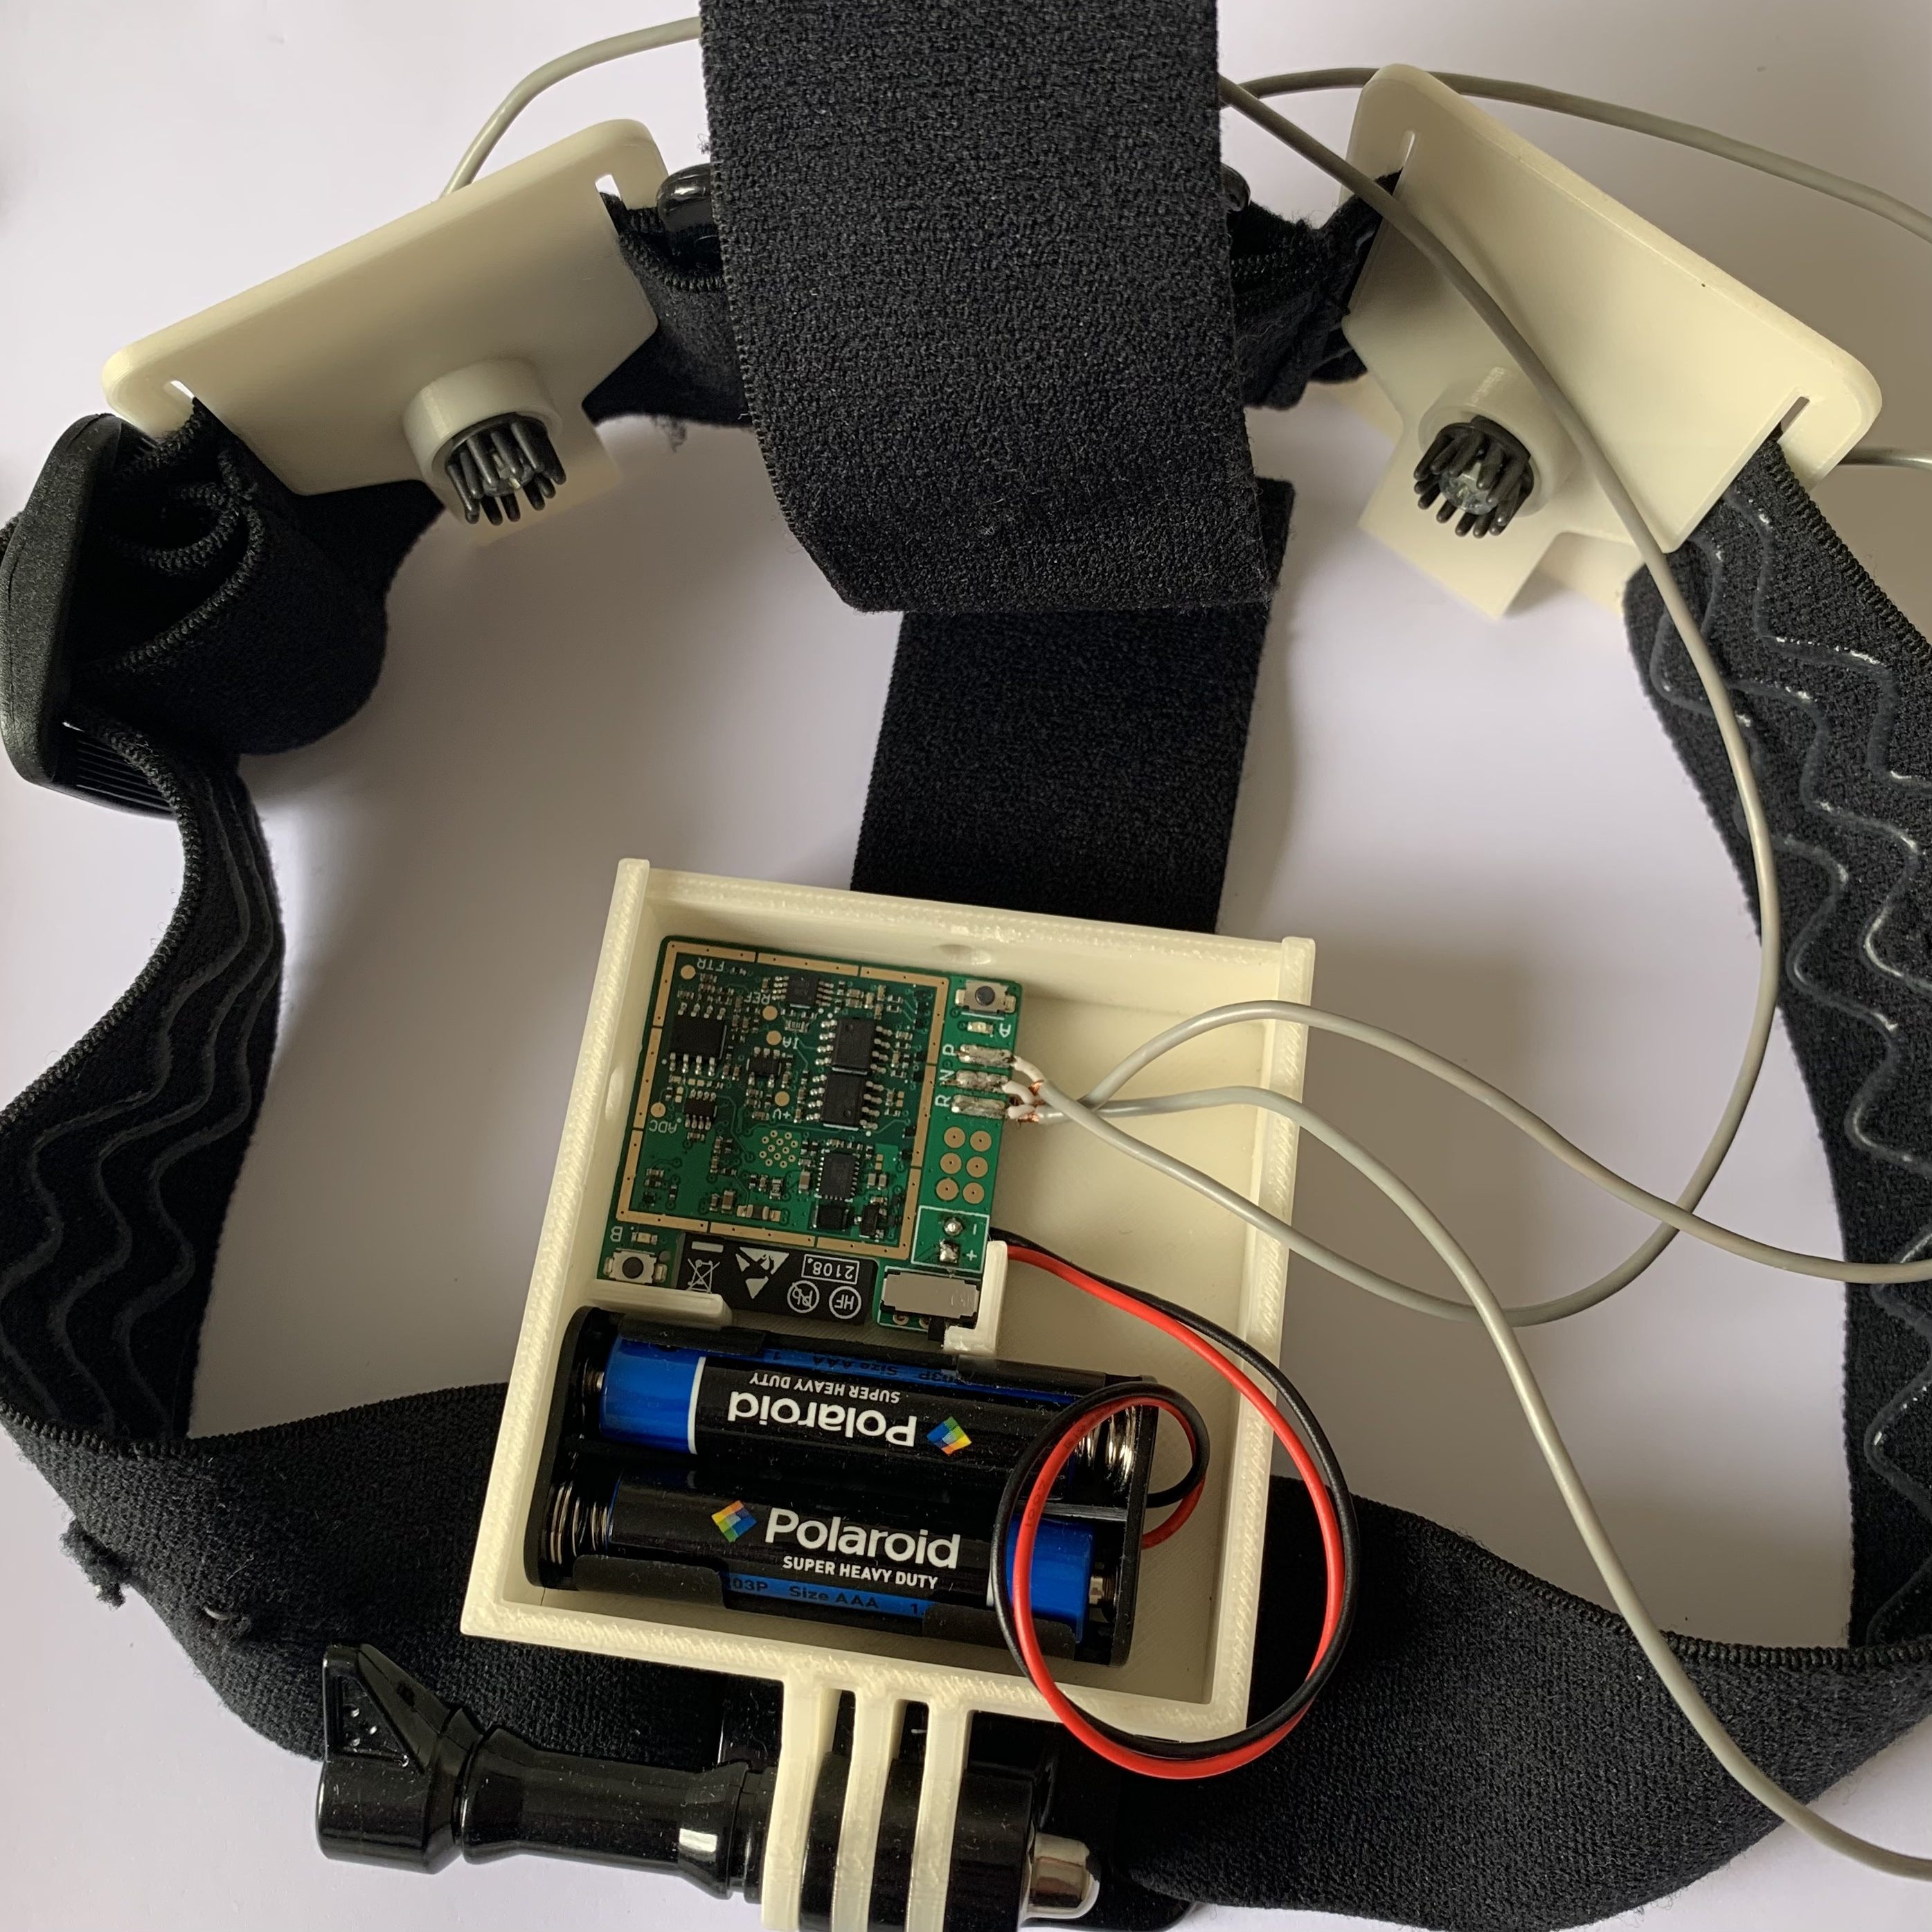
\includegraphics[width=\textwidth]{final-headband}
         \caption{View of the 3D-printed headband housing and adjustable elastic strap. The electronic hardware is externally powered by two 1.5V AAA alkaline batteries before being boosted to 3.3V using on-board circuitry.}
         \label{fig:final-headband}
     \end{subfigure}
     \hfill
    \begin{subfigure}[c]{0.48\textwidth}
         \centering
         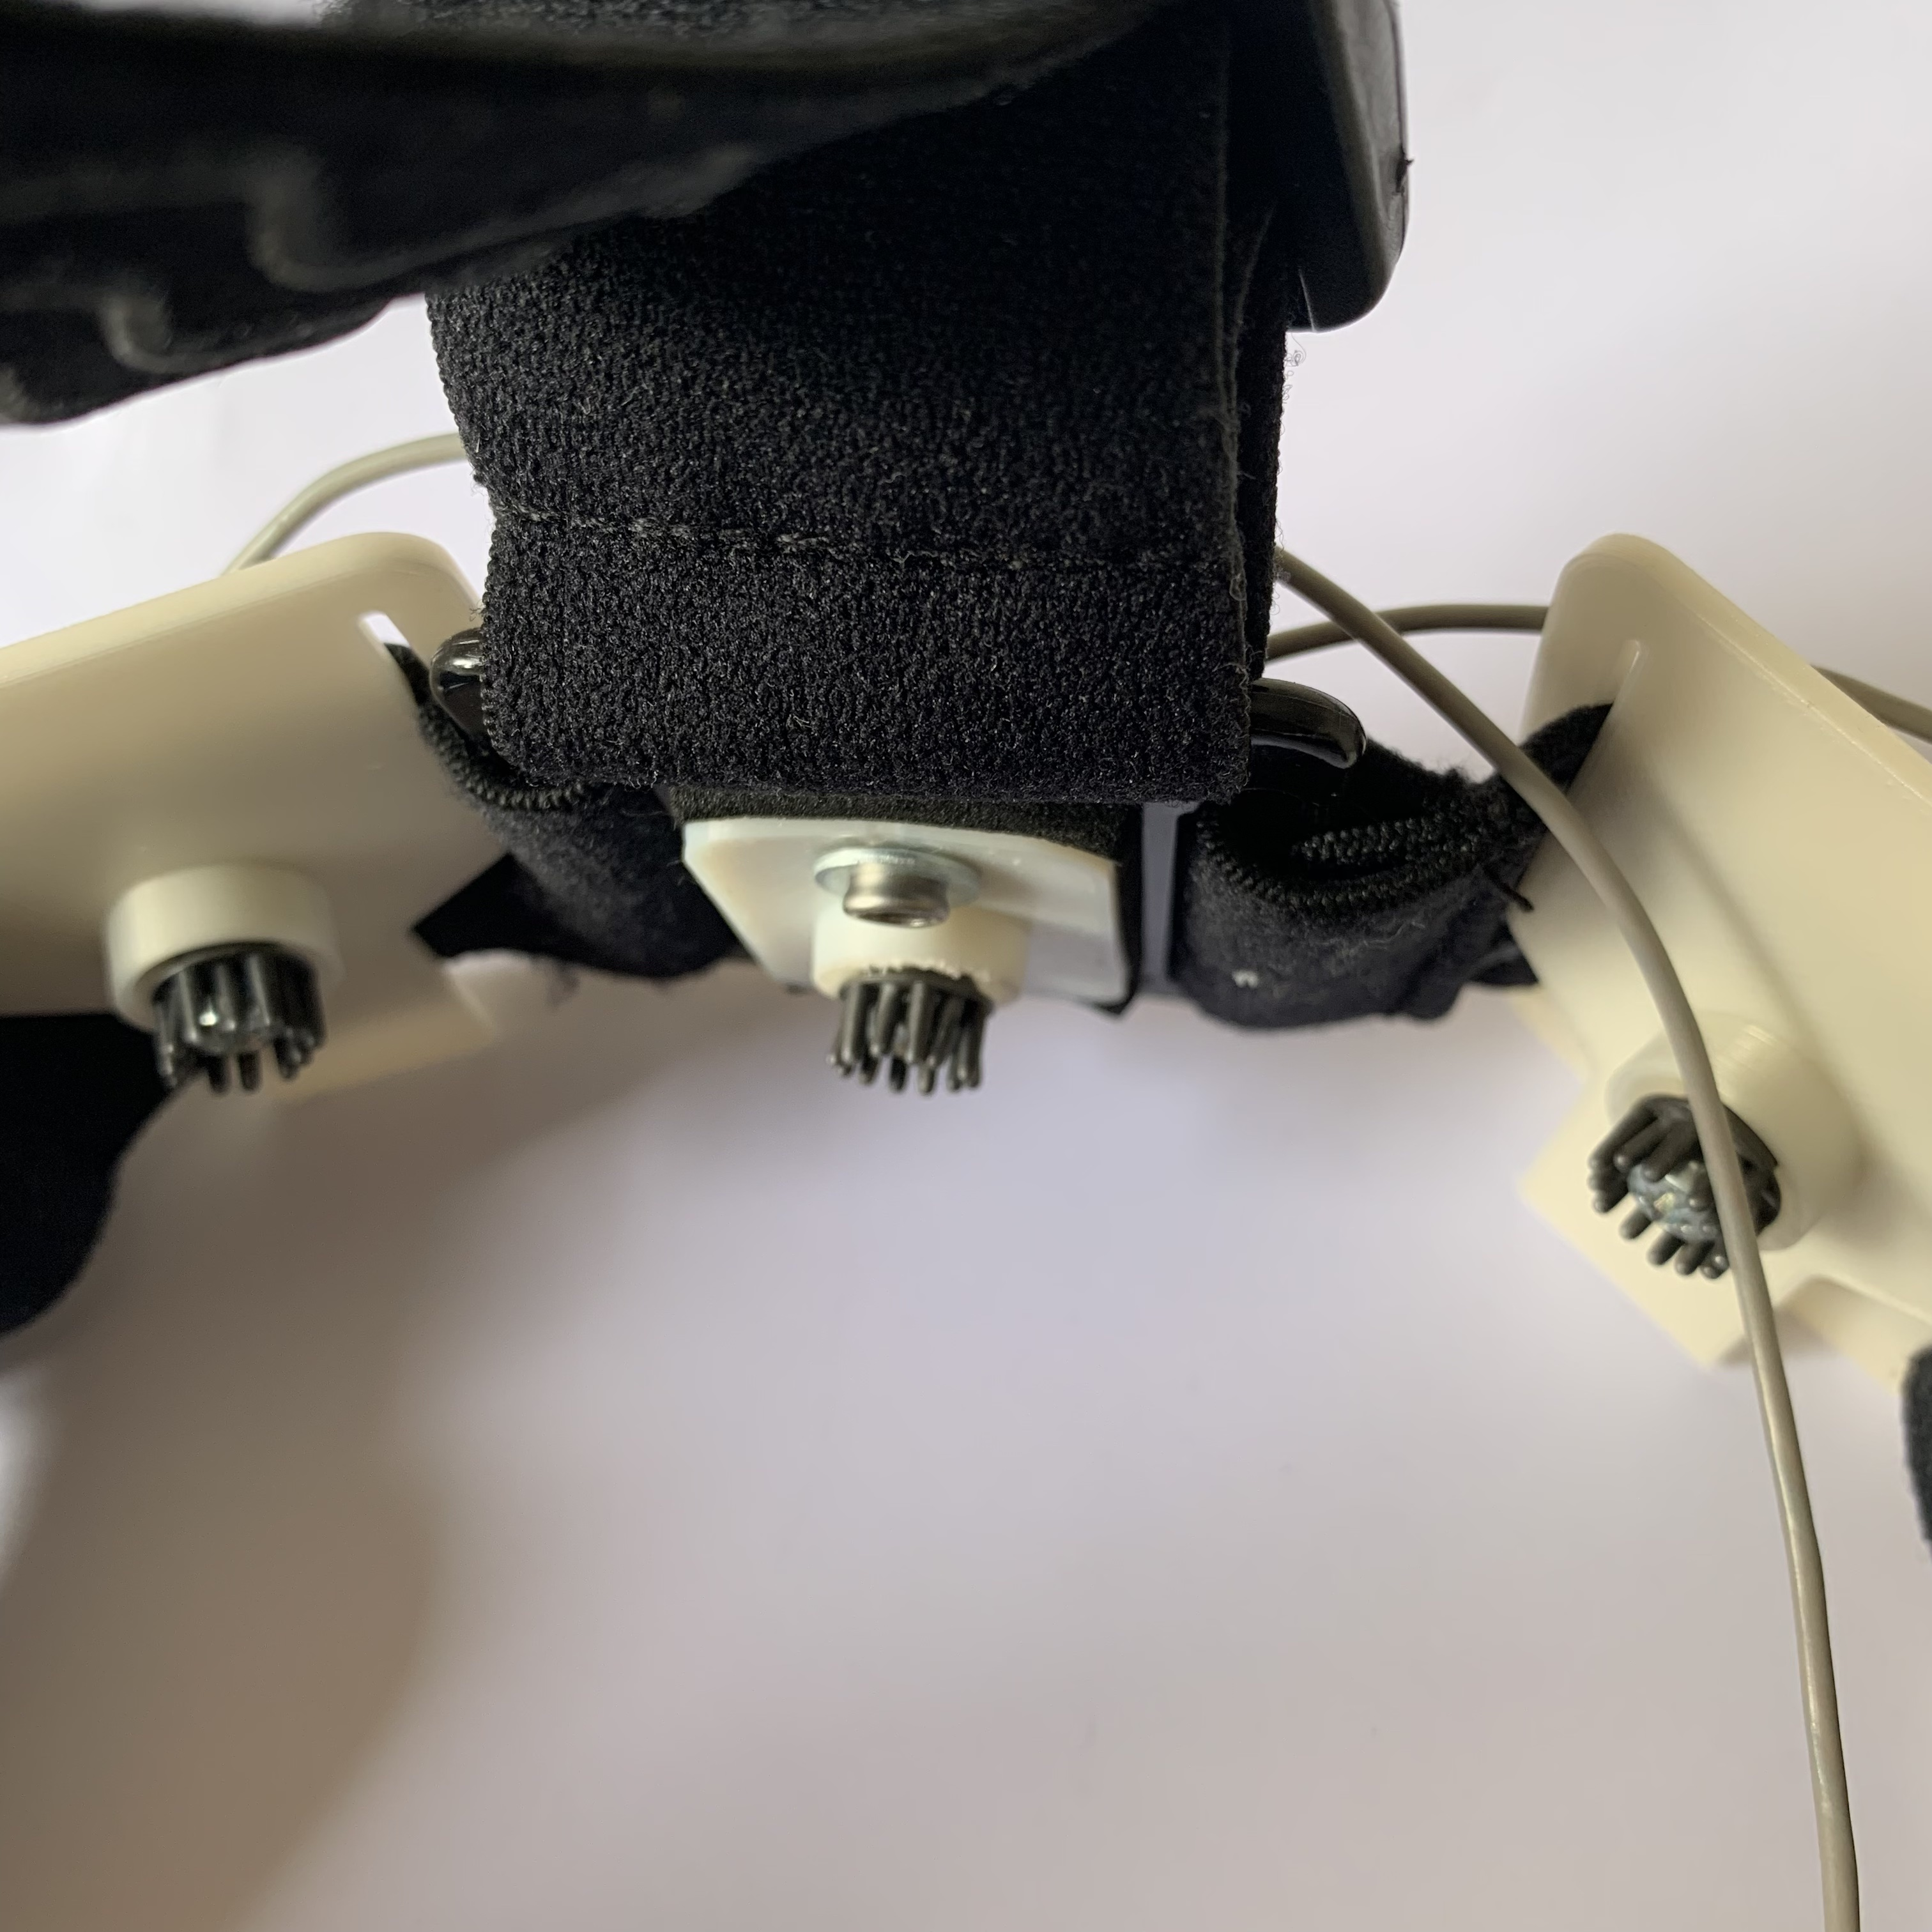
\includegraphics[width=\textwidth]{final-headband-elec}
         \caption{Close-up view of the two active electrodes on either side of the reference electrode. Electrodes are housed in 3D-printed locator structures that allow for slight pitch and yaw deviations about the axis normal to the scalp.}
         \label{fig:final-headband-electrodes}
     \end{subfigure}
        \caption{Images of the final complete hardware system comprising electronic and mechanical EEG hardware. All hardware was designed by the NGNI Lab. The band is intended to be worn such that the electrodes make contact with the back of the scalp in the occipital or parieto-occipital region.}
        \label{fig:final-headband-subfigs}
\end{figure}

\section{Experimental Procedure}
\subsection{Data acquisition}
Owing to limitations imposed by the Coronavirus Pandemic, all experimental data was recorded on the author. The SSVEP stimulus squares interface shown in Figure \ref{fig:ssvep-squares-c5} was displayed on an 11" Apple iPad Pro ($4^{\textrm{th}}$ generation, 2020) with Apple A12Z CPU, 2388x1688 px (264 PPI) display resolution and 120Hz refresh rate. The web page was displayed in the native Safari browser with no other apps running simultaneously so as to minimise CPU load and provide consistent flicker frequency across the stimulus squares. With reference to the diagram in Figure \ref{fig:visual-setup-diagram}, the iPad was positioned $d=50$cm away from the subject's visual field at an angle of $\theta=45$ degrees below the horizontal line-of-sight. It should be noted, however, that this arrangement was followed approximately and is only provided as a rough guideline.

\begin{figure}[!htb]
    \centering
    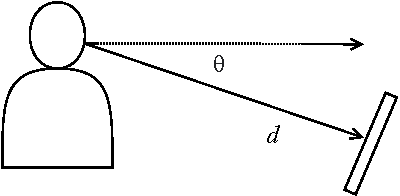
\includegraphics[width=0.3\textwidth]{visual-setup-diagram}
    \caption[Diagram showing the arrangement of the stimulus display device relative to a subject undergoing the experiment]{Diagram showing the arrangement of the stimulus display device relative to a subject undergoing the experiment. The dotted line represents the line-of-sight normal to the subject's eye line and the solid arrow is the position vector normal to the display device held distance $d$ away from the visual field at angle $\theta$ below the line-of-sight.}
    \label{fig:visual-setup-diagram}
\end{figure}

\newpage
\subsection{Testing and verification}
\label{subsection:testing-verification-method-c4}
In order to verify that signals measured from by the BCI system were valid, several checks were devised. 

\subsubsection{Basic firmware test}
The first very basic test involved verifying the integrity of the firmware on board the ESP32. This involved testing basic peripheral functionality such as toggling an LED connected to a GPIO pin and sampling a known, fixed value from the ADC. Storage and retrieval of data from flash, checking floating point precision and verifying operations from third party modules were also checked. 

\subsubsection{Alpha band test}
As mentioned briefly in Section \ref{subsection:nature-of-eeg-signals}, EEG signal energy related to visual processing typically occurs in the \textit{alpha} band between 8 and 13Hz and can be measured around the occipital region of the brain. As alpha energy is pronounced when the eyes are closed and attenuated when they are open, this phenomenon can be used as a basic test of the validity of a BCI. If signal energy as measured by the BCI in the occipital region follows this pattern, it suggests that acquired signals are not simply random noise. It should be noted, however, that individuals show varying levels of alpha reactivity and the difference in energy under these two conditions may not be significant in all individuals. 

\subsubsection{Digital signal processing tests}
In order to test the integrity of digital signal processing (DSP) elements in the BCI system (explored more in detail in Chapter \ref{chapter:system-design}), the following preliminary checks were employed. In all of the following tests, data was recorded on the electronic hardware detailed above and was analysed offline.
\begin{itemize}
    \item in order to test the on-device digital low-pass filter, data was recorded with and without the filter active. Analysis was performed to verify that signal components beyond the target frequency band were suitably attenuated and that pass-band distortion was acceptable. 
    \item in order to verify the equivalence between original and down-sampled versions of the same signal, data was collected under three conditions: (i) sampling at $f_s=256$Hz with low pass filtering but no downsampling, (ii) sampling at $f_s=256$Hz with low pass filtering and downsampling to $f_s'=64$Hz and (iii) sampling at $f_s=256$Hz with \textit{no} low-pass filtering and downsampling to $f_s'=64$Hz.
\end{itemize}

\subsubsection{Artificial signal decoding test}
In order to test the hardware and signal decoding elements, a square wave signal at a known frequency $f_0$ was produced and applied across the active electrodes. The resulting signal spectrum was measured and compared to the theoretical spectrum of a square wave at frequency $f_0$. This was performed with and without low-pass filtering to determine if high frequency harmonics were being attenuated correctly. SSVEP signal decoding algorithms were also tested by ensuring that they produced a decoded output matching the artificial stimulus frequency $f_0$.

\subsection{Demonstration procedure}
During the Royal Society exhibition, audience members attending remotely from various locations will be presented a mobile-friendly, lightweight web page with several flickering squares that will form the SSVEP stimuli. These squares will be programmed to flicker at predetermined stimulus frequencies $f_1, \dots, f_n$. Each stimulus will correspond to an action - such as `up' or `down' - that will control an avatar in a cooperative multiplayer game or simulation. The core objective of the designed BCI system is to decode $f_1, \dots, f_n$ in order to interpret each user's desired action (i.e. discern which stimulus square they are focused on).

% % Chapter 5: System Design
% %% Chapter 5: System design
\chapter{System Design}
\label{chapter:system-design}

\graphicspath{ {report/C5 System Design/assets/} } 

\section{Design of the SSVEP Stimuli}

Naturally, an important part of the SSVEP-based BCI system is the SSVEP stimuli which will be presented to individuals participating in the exhibition (or in general, anyone interacting with the system thereafter). Taking into account design parameters such as stimulus colour, position and contrast mentioned in the literature cited in Section \ref{subsection:evoking-measuring-ssveps}, a basic user interface (UI) was designed with a series of flashing squares as depicted in Figure \ref{fig:ssvep-squares-c5}. This UI was implemented as a lightweight HTML page with basic CSS styling and Javascript to handle animation (flickering of the squares). This decision was made to allow for the simplest and most convenient deployment across any device capable of displaying a web page (mobile or otherwise). The number of blocks being displayed and their labels are subject to adjustment in accordance with other elements of the demonstration beyond the scope of this project.

\begin{figure}][!htb]
    \centering
    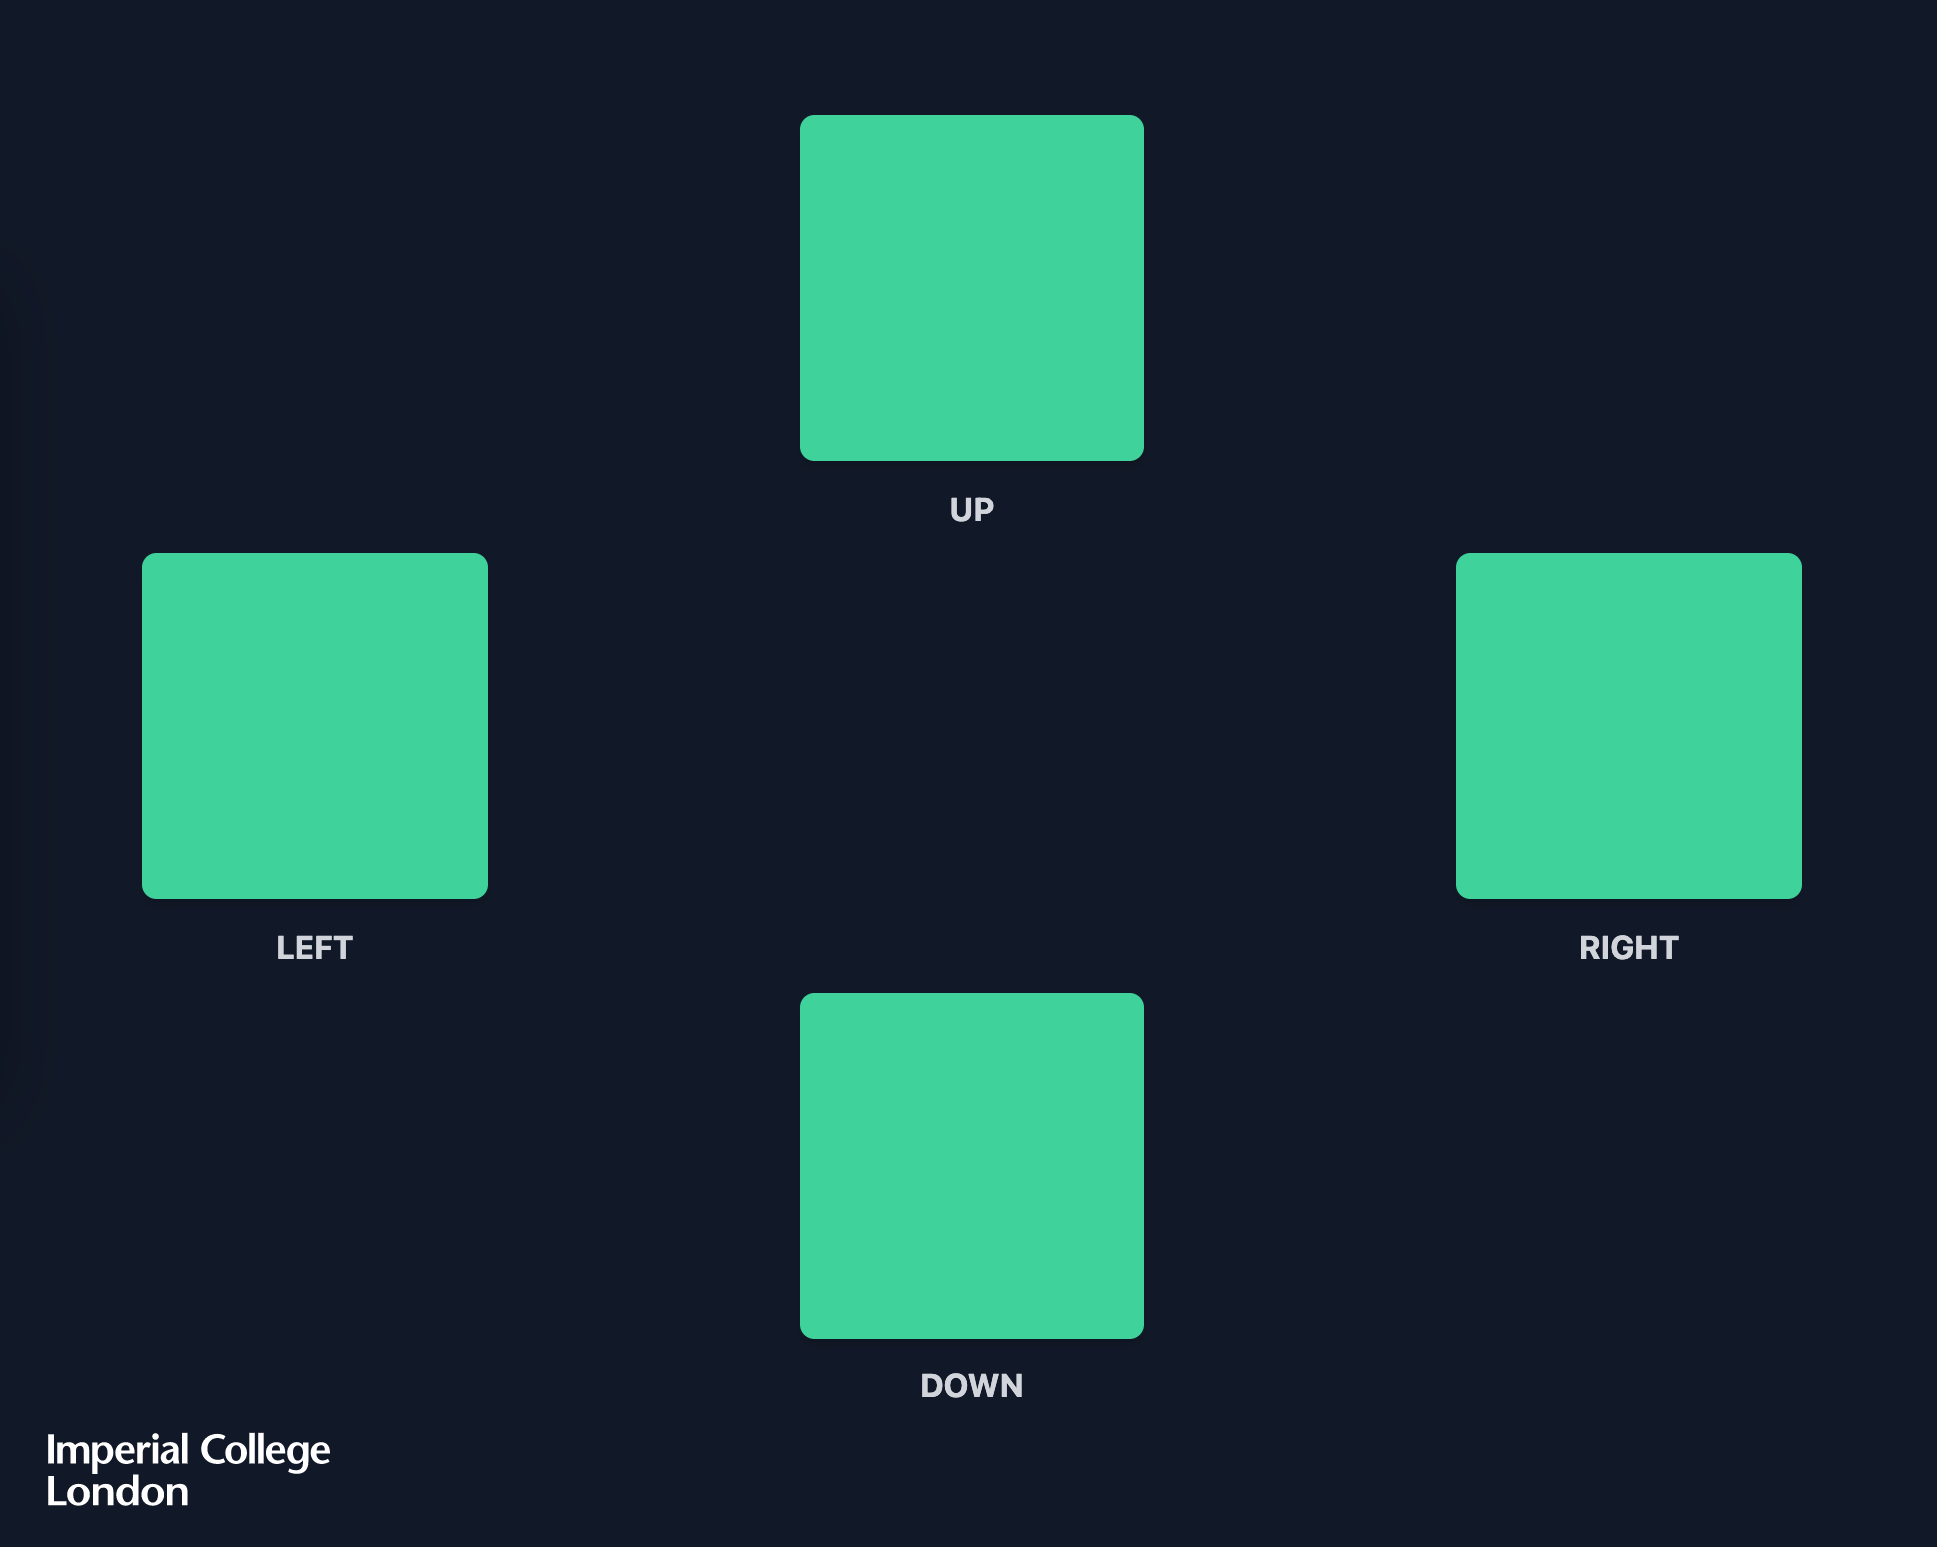
\includegraphics[width=0.8\textwidth]{ssvep-squares}
    \caption{Screen capture of the user interface for displaying SSVEP stimuli. The blocks can be independently set to any flicker frequency of interest.}
    \label{fig:ssvep-squares-c5}
\end{figure}

A key consideration in the design of the SSVEP stimuli is the stimulus frequencies $f_1, \dots, f_n$ to use. As mentioned in Section \ref{subsection:time-frequency-considerations-c2}, similar studies typically use stimulus frequencies between 6Hz and 15Hz for this task. Based on frequencies most commonly selected, the set of stimulus frequencies $\mathcal{F}$ selected for this project were: $\mathcal{F} = \{f_1, \dots, f_n\} = \{7, 8, 10, 12\}$ (all in Hz). Note that, external factors related to this project may only require some subset of $\mathcal{F}$: for example, the stimulus square corresponding to `down' may be omitted if only the other three actions are required in the game or simulation. 

\section{Digital Signal Processing System}

A crucial part in the design of the BCI system is the digital signal processing (DSP) system. The key functions of this system are to digitise, filter and resample the analogue output of the analogue signal processing system presented in Figure \ref{fig:analogue-system-c4}. An overview of the DSP system is shown in Figure \ref{fig:digital-system-c5}.

\begin{figure}
    \centering
    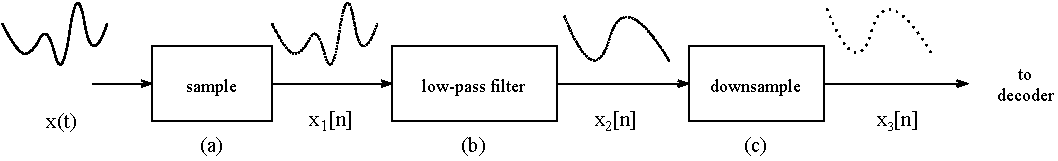
\includegraphics[width=\textwidth]{digital-system}
    \caption{Digital signal processing system}
    \label{fig:digital-system-c5}
\end{figure}

Details of the components shown in Figure \ref{fig:digital-system-c5} are provided below. 

\subsubsection{Sampling}
The analogue signal $x(t)$ digitised to $x_1[n]$ using the 12-bit SAR ADC on-board the ESP32. A sampling frequency of $f_s=256$Hz was selected based for several reasons. First, this is a typical value mentioned in the literature as noted in Section \ref{subsection:time-frequency-considerations-c2}. Second, and more importantly, considering the SSVEP target frequency band 

\subsubsection{Digital low-pass filtering}

\subsubsection{Downsampling}


\begin{enumerate}[label=(\alph*)] % (a), (b), (c), ...
\item sampling
\begin{itemize}
   
\end{itemize}
\item low-pass filter
\begin{itemize}
    \item low-pass filter to isolate the frequency band of interest from DC to $28$Hz. Used to provide greater 50Hz noise rejection to allow for downsampling. 
    \item corner frequency $f_c=32$Hz
    \item $10^{\textrm{th}}$ order elliptical filter
    \item 50Hz rejection characteristics: minimum 17dB, nominal 35dB and maximum 55dB.
\end{itemize}

\item adjustable-gain output amplifier
\begin{itemize}
    \item adjustable gain between 1.745 and 19.2
    \item input low-pass filter dynamics: corner frequency of $f_c=36.35$Hz 
\end{itemize}
\end{enumerate}

\section{Firmware structure}
Discuss Micropython and uLab here, including their features, benefits and potential drawbacks compared to more conventional C/C++.
Discuss module structure and give a diagram of how modules are arranged and what functionality they provide

\subsection{Networking}
Discuss AWS IoT interface and real-time streaming capabilities using MQTT



\section{Algorithm Implementation}



Discuss numerical challenges, precision issues, memory constraints
Discuss some of the auxiliary computational approaches used such as eigenvalue solvers etc



%% Chapter 6: Results
%% Chapter 6: Results
\chapter{Results}
\label{chapter:results}

\graphicspath{ {report/C6 Results/assets/} } 

% ** remember to include results of all early, prelim experiments including the OpenBCI experiments and periodogram plots of the alpha energy experiments with the initial Frankenstein hardware.

\section{Hardware Verification and Testing}
This section details the results of the various verification tests mentioned in Section \ref{subsection:testing-verification-method-c4}. The purpose of these tests was to verify that all core components of the designed system performed as expected. After basic tests to verify firmware integrity and communication with the ESP32-based target board passed, the digital signal processing (DSP) system was investigated. The results of important diagnostic tests are detailed below. Throughout this section, "the hardware" refers to the electronic hardware introduced in Section \ref{subsection:electronic-hardware-proto} and pictured in Figure \ref{fig:esp-hardware}.

\subsection{DSP system}
As explained in Section \ref{fig:digital-system-c5}, the DSP system is crucial for preparing analogue signals acquired from hardware prior to decoding. In order to test several components of this system simultaneously, a square wave signal $x[n]$ at fundamental frequency $f_x^{(0)}=12$Hz was fed to the ADC of the ESP32. Sampling was set to $f_s=256$Hz and where applicable, downsampling to $f_s^'=64$Hz was used. Owing to the lack of access to a signal generator or other laboratory equipment, the input signal $x[n]$ was generated using a hardware timer on board the ESP32. This experiment was designed to test the following components of the DSP system as follows:
\begin{enumerate}
    \item \textbf{sampling}: a basic sanity check to verify that a square wave at 12Hz was indeed measured by the ADC. This also offered a means of inspecting the consistency (both in amplitude and frequency) of the measured signal.
    \item \textbf{filtering}: the input signal $x[n]$ was filtered by the onboard digital low-pass filter described in Section \ref{subsection:digital-filtering} to yield $y[n]$. Given the filter's corner frequency of $f_c=26$Hz, $y[n]$ should only contain the fundamental frequency $f_x^{(0)}=12$Hz since higher order harmonics of the square wave input at $\{f_x^{(k)} |f_x^{(k)}=(2k-1)f_x^{(0)}, \, k=2,3, \dots\} = \{36\text{Hz}, 60\text{Hz}, \dots\}$ should be fully attenuated. Furthermore, the measured spectrum of $y[n]$ offers a way to compare the actual and designed behaviour of the filter.
    \item \textbf{downsampling}: a simple check to confirm that, given all prior design decisions, downsampling does not distort the originally measured signal excessively in the frequency band of interest (around $7-12$Hz). With low-pass filtering in place, there should be no aliasing or artefacts introduced.
\end{enumerate}

All results reported below were computed on the hardware itself, i.e.: all DSP operations (sampling, filtering, resampling) were computed on-device as would happen in a real application. Figures were then plotted using \texttt{Matplotlib}, an open source Python library.

\subsubsection{Sampling}
Figure \ref{fig:sq-wave-time-c6} shows the filtered signal $y[n]$ against the measured input square wave $x[n]$. From visual inspection, $x[n]$ appears to have very consistent frequency and amplitude as desired. $y[n]$ shows marginal phase lag and slight inconsistencies in amplitude compared to the ideal output $y^*[n] = \frac{4}{\pi}\sin(2\pi f_x^{(0)}n)$. However, these slight deviations are certainly tolerable and would make little to no difference to the success of subsequent decoding algorithms.

\begin{figure}[h]
    \centering
    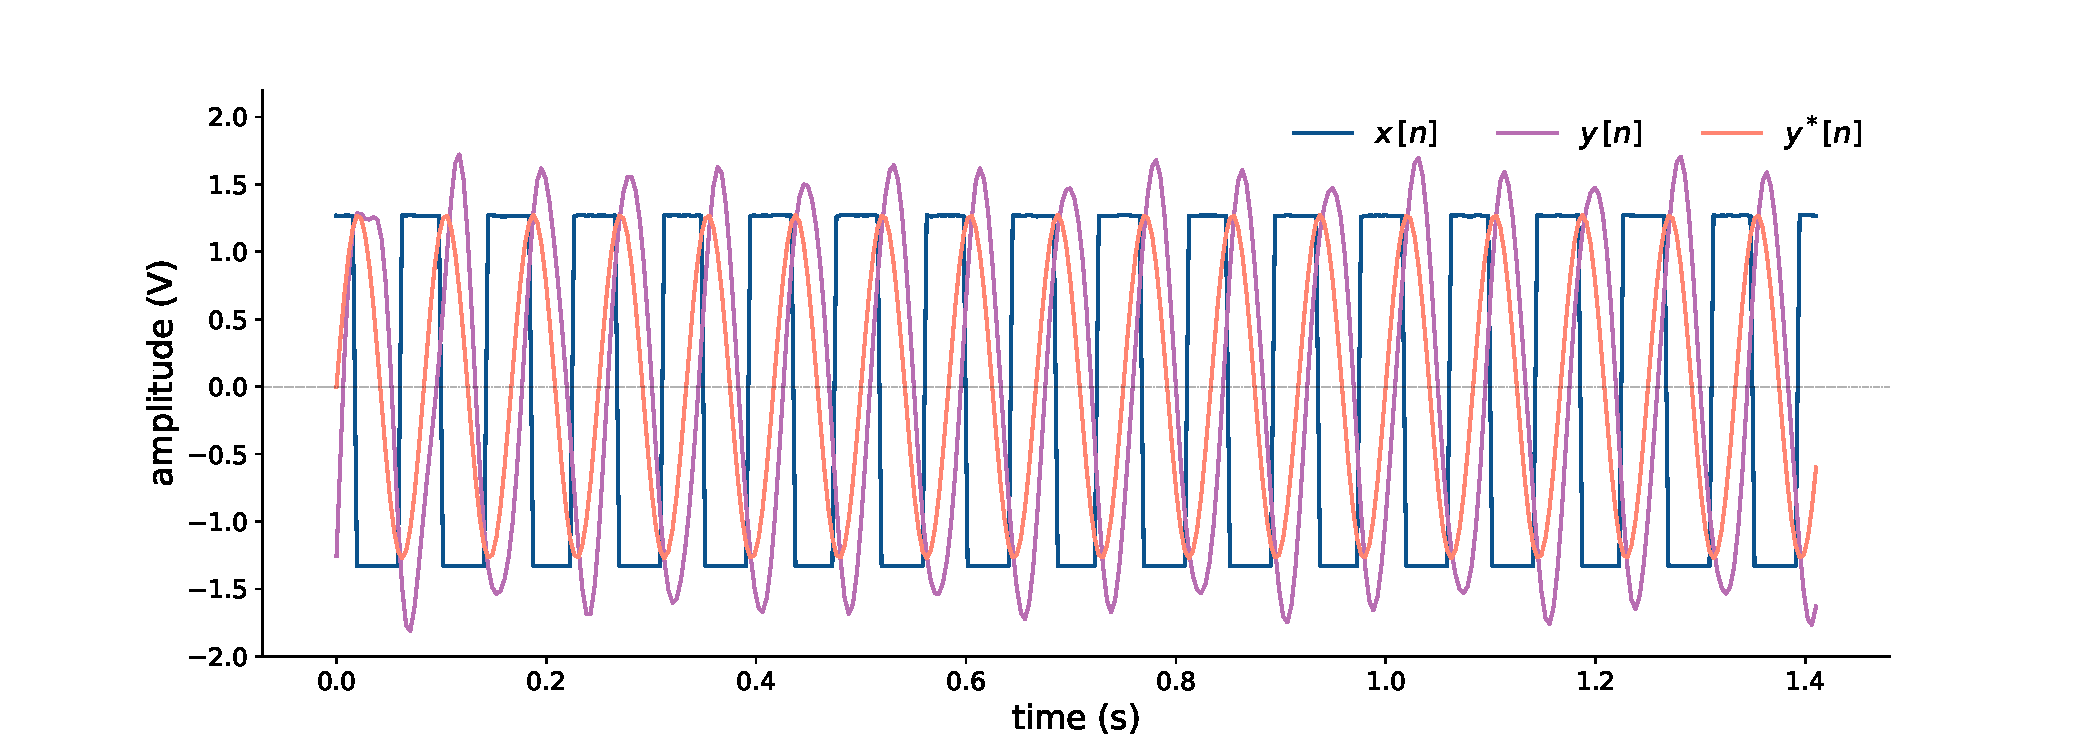
\includegraphics[width=\textwidth]{sq_wave_filtering_time}
    \caption[Time domain plot showing the measured square wave signal together with the digitally-filtered output signal.]{Time domain plot showing the measured square wave signal $x[n]$ together with the digitally-filtered output signal $y[n]$ designed to retain only the fundamental frequency $f_x^{(0)}$ of $x[n]$. The ideal output signal $y^*[n]$ represents a sinsuoid at frequency $f_x^{(0)}$: $y^*[n] = \frac{4}{\pi}\sin(2\pi f_x^{(0)}n)$.}
    \label{fig:sq-wave-time-c6}
\end{figure}

\subsubsection{Filtering}
Figure \ref{fig:sq-wave-spectra-c6} shows PSD estimates $\hat{P}_x(\omega)$ and $\hat{P}_y(\omega)$ of $x[n]$ and $y[n]$ respectively in the form of periodograms. Confirming the time domain representation in Figure \ref{fig:sq-wave-time-c6}, $\hat{P}_x(\omega)$ shows power peaks at the odd numbered harmonics of $x[n]$. This can be explained by the Fourier series expansion of an ideal square wave at fundamental frequency $f^{(0)}$ with 50\% duty cycle:
\begin{equation}
    x[n]=\frac{4}{\pi} \sum_{k=1}^{\infty} \frac{\sin (2 \pi(2 k-1) f^{(0)} n)}{2 k-1},
    \label{eq:fourier-series-sinsusoid}
\end{equation}
which is nothing but an infinite sum of sinusoids whose amplitudes decay with frequency. Notice that only odd-numbered harmonics in (\ref{eq:fourier-series-sinsusoid}) are non-zero. Therefore, the ideal spectrum $P_x(\omega)$ of $x[n]$ should be an impulse train at frequencies $(2k-1)f_x^{(0)}, \, k\geq2, \, k\in\mathbb{Z}$. 

While not quite impulses, power peaks of $\hat{P}_x(\omega)$ in Figure \ref{fig:sq-wave-spectra-c6} are clearly visible at the odd-numbered harmonics at 26Hz, 60Hz and so on. The spectrum of the filtered signal, $\hat{P}_y(\omega)$, shows very little distortion in the pass-band between 0 and $f_c=26$Hz, as well as impressively steep roll-off for $f>f_c$. As a result, only the fundamental frequency of $x[n]$ is captured in $y[n]$, as desired. Attenuation of higher frequency harmonics in $x[n]$ by the digital filter is evidently very effective and meets the design criteria stated in Section \ref{subsection:digital-filtering}: stop-band attenuation is approximately 80dB, as can be seen in the power difference between $\hat{P}_x(\omega)$ and $\hat{P}_y(\omega)$ at 60Hz, for example.

\begin{figure}[!htb]
    \centering
    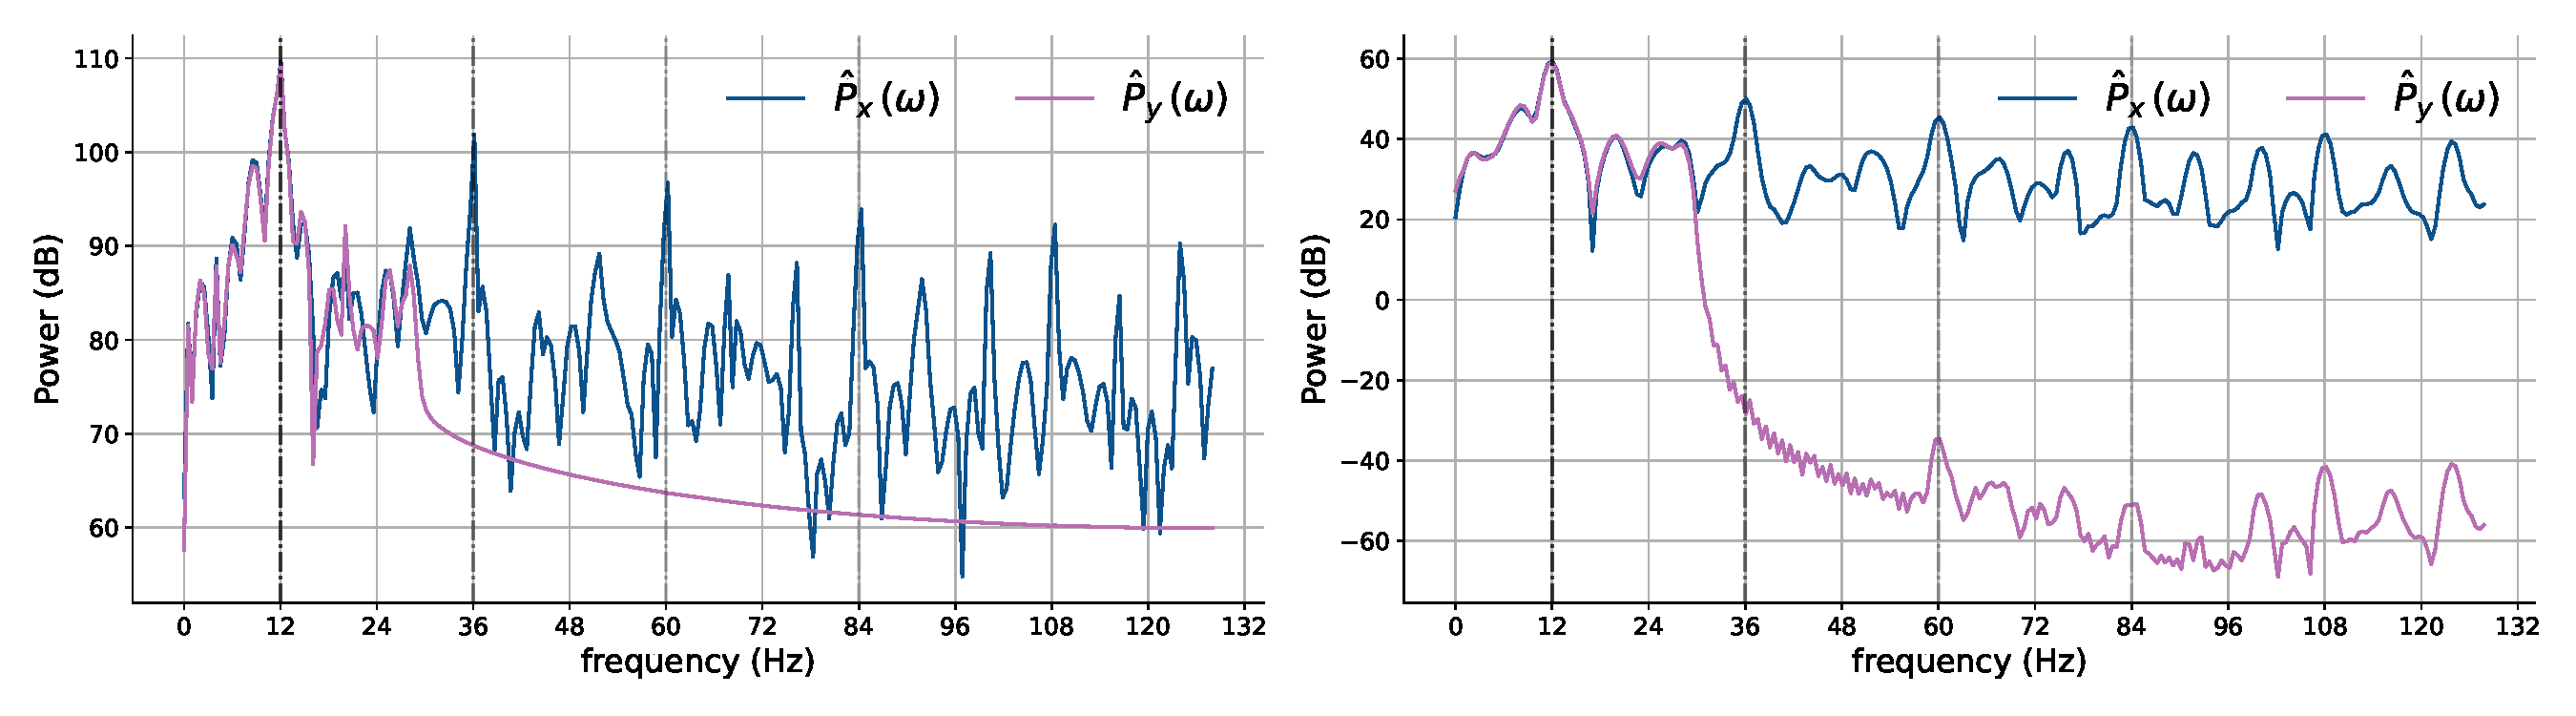
\includegraphics[width=\textwidth]{sq_wave_filtering_spectra}
    \caption[PSD estimates of a measured input signal and its filtered output]{Standard periodogram (left) and Welch-averaged periodogram (right) representing PSD estimates of measured input signal $x[n]$ and filtered output $y[n]$. Dashed vertical lines mark $f_x^{(0)}$ and odd-numbered harmonics of $x[n]$.}
    \label{fig:sq-wave-spectra-c6}
\end{figure}

\subsubsection{Downsampling}

\begin{figure}[h]
    \centering
    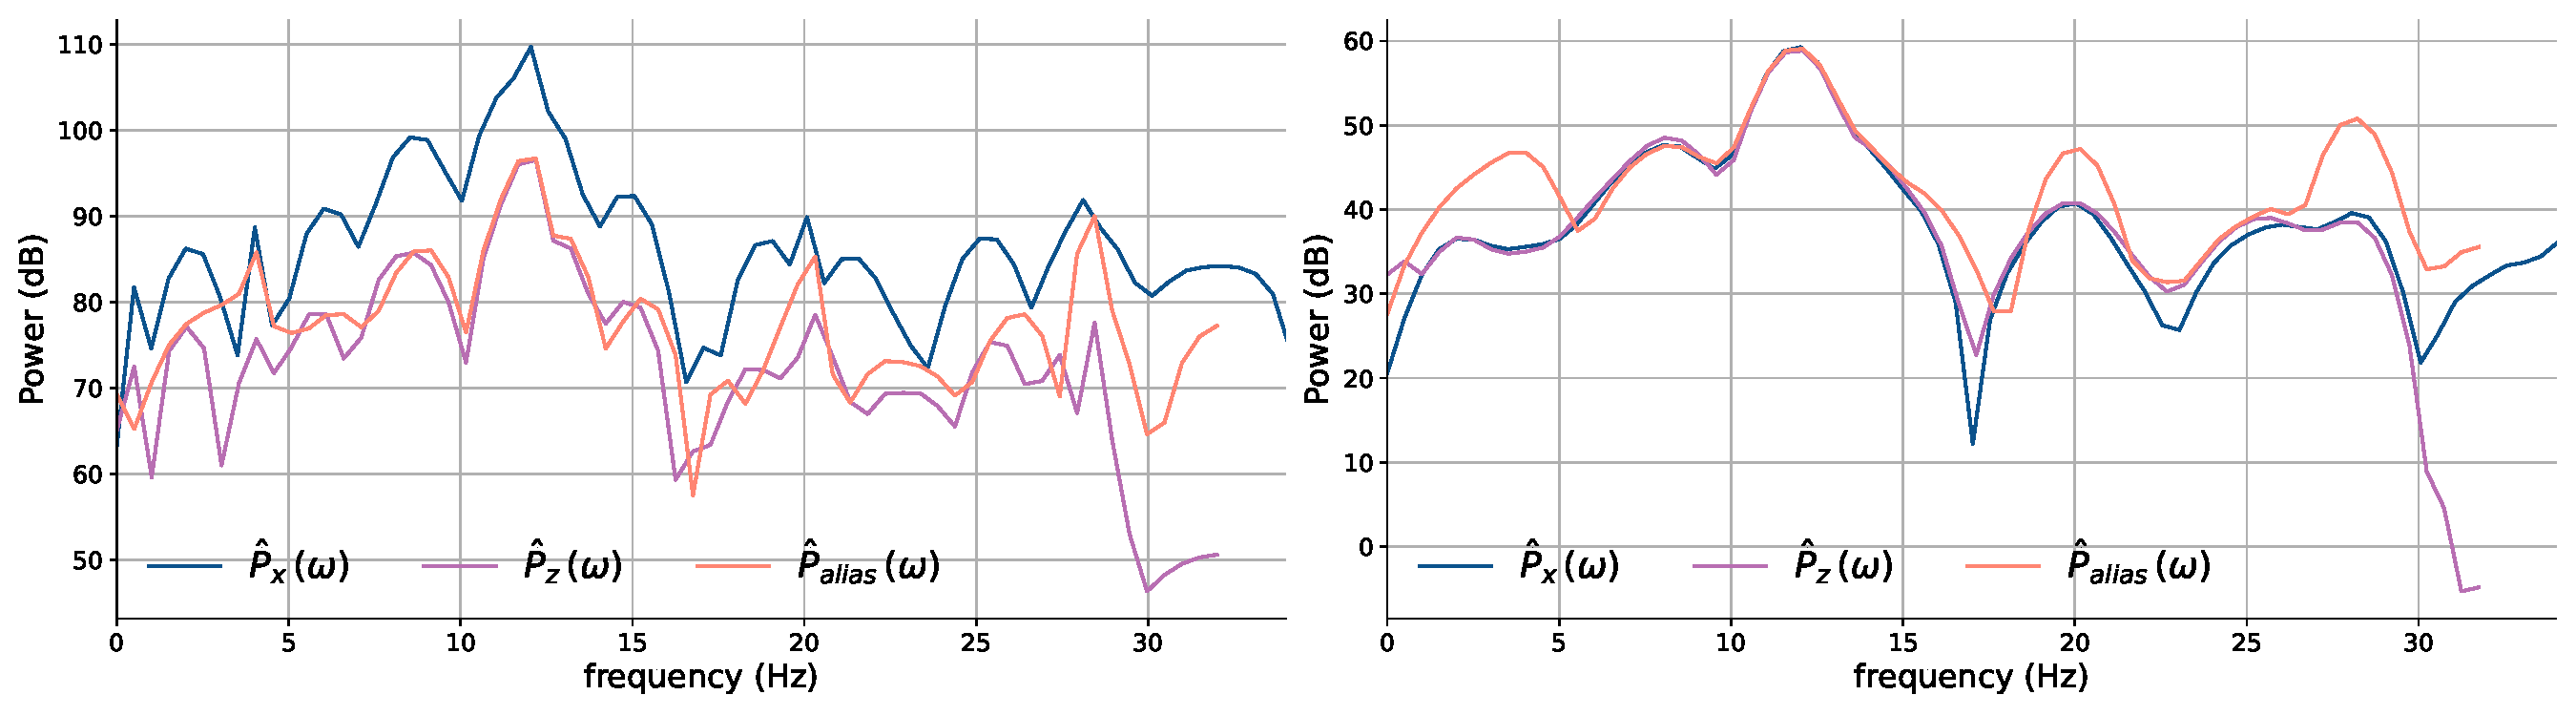
\includegraphics[width=\textwidth]{sq_wave_filtering_ds_spectra}
    \caption[PSD estimates of an input signal, filtered and downsampled version and a downsampled version without filtering.]{Standard periodogram (left) and Welch-averaged periodogram (right) representing PSD estimates $\hat{P}_x(\omega)$ and $\hat{P}_z(\omega)$ of input $x[n]$ and filtered, downsampled output $z[n]$ respectively. $\hat{P}_{\text{alias}}(\omega)$ shows the estimated spectrum of a downsampled version of $x[n]$ \textit{without} prior low-pass filtering}.
    \label{fig:sq-wave-ds-spectra-c6}
\end{figure}

\subsection{Hardware and data acquisition}

\begin{figure}[htp]
\subfloat[eyes open]{%
  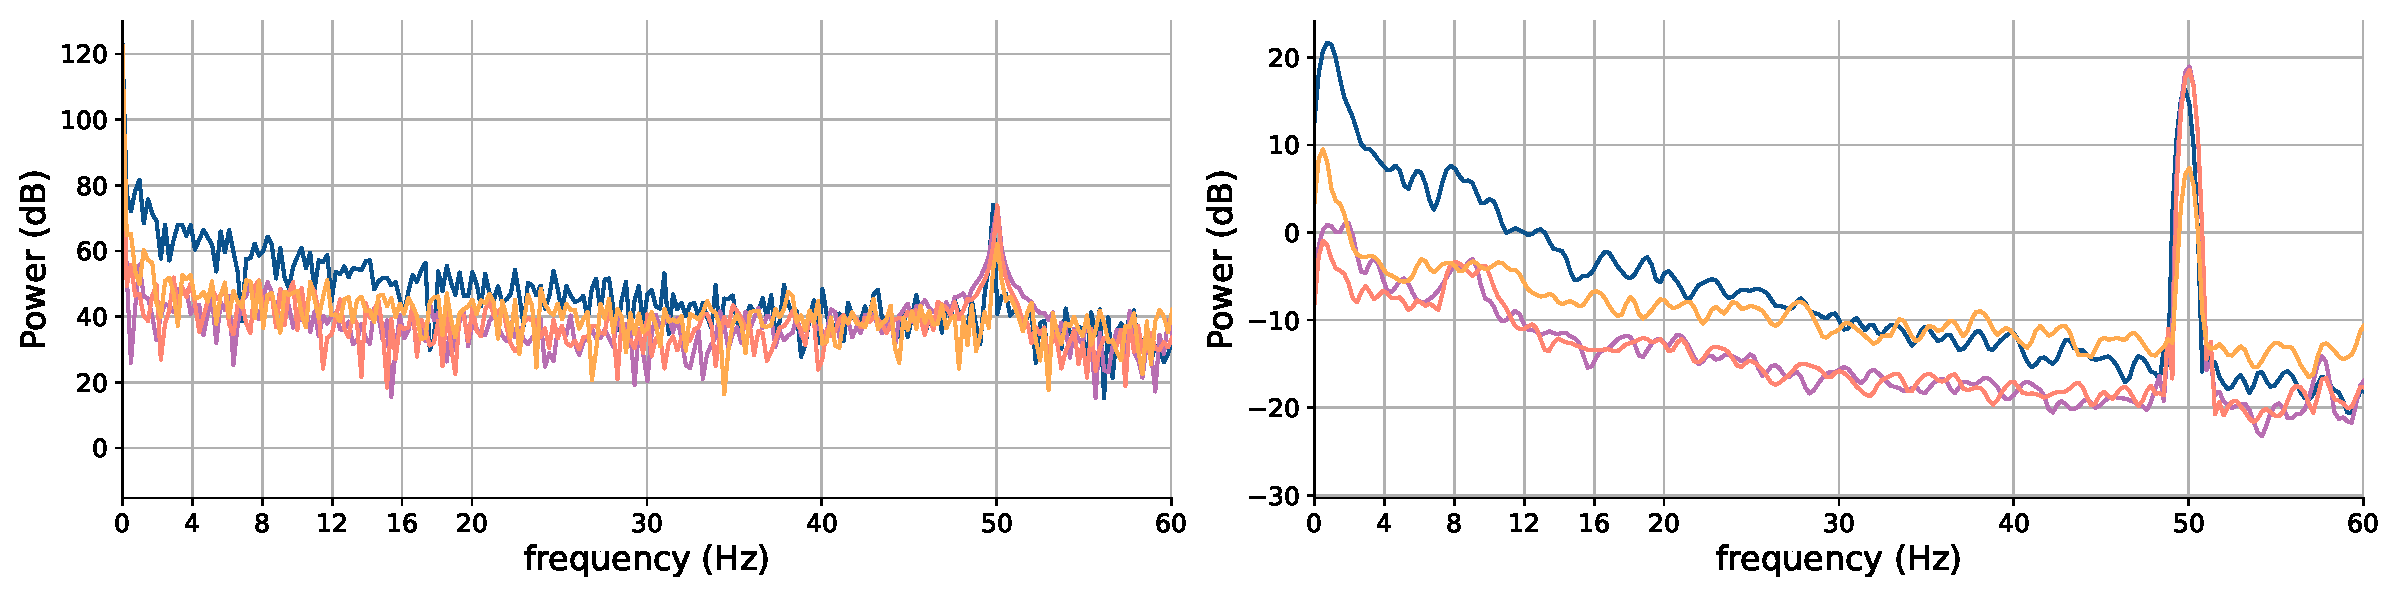
\includegraphics[clip,width=\columnwidth]{eyes_open_alpha_spectra_N1024.pdf}%
}

\subfloat[eyes closed]{%
  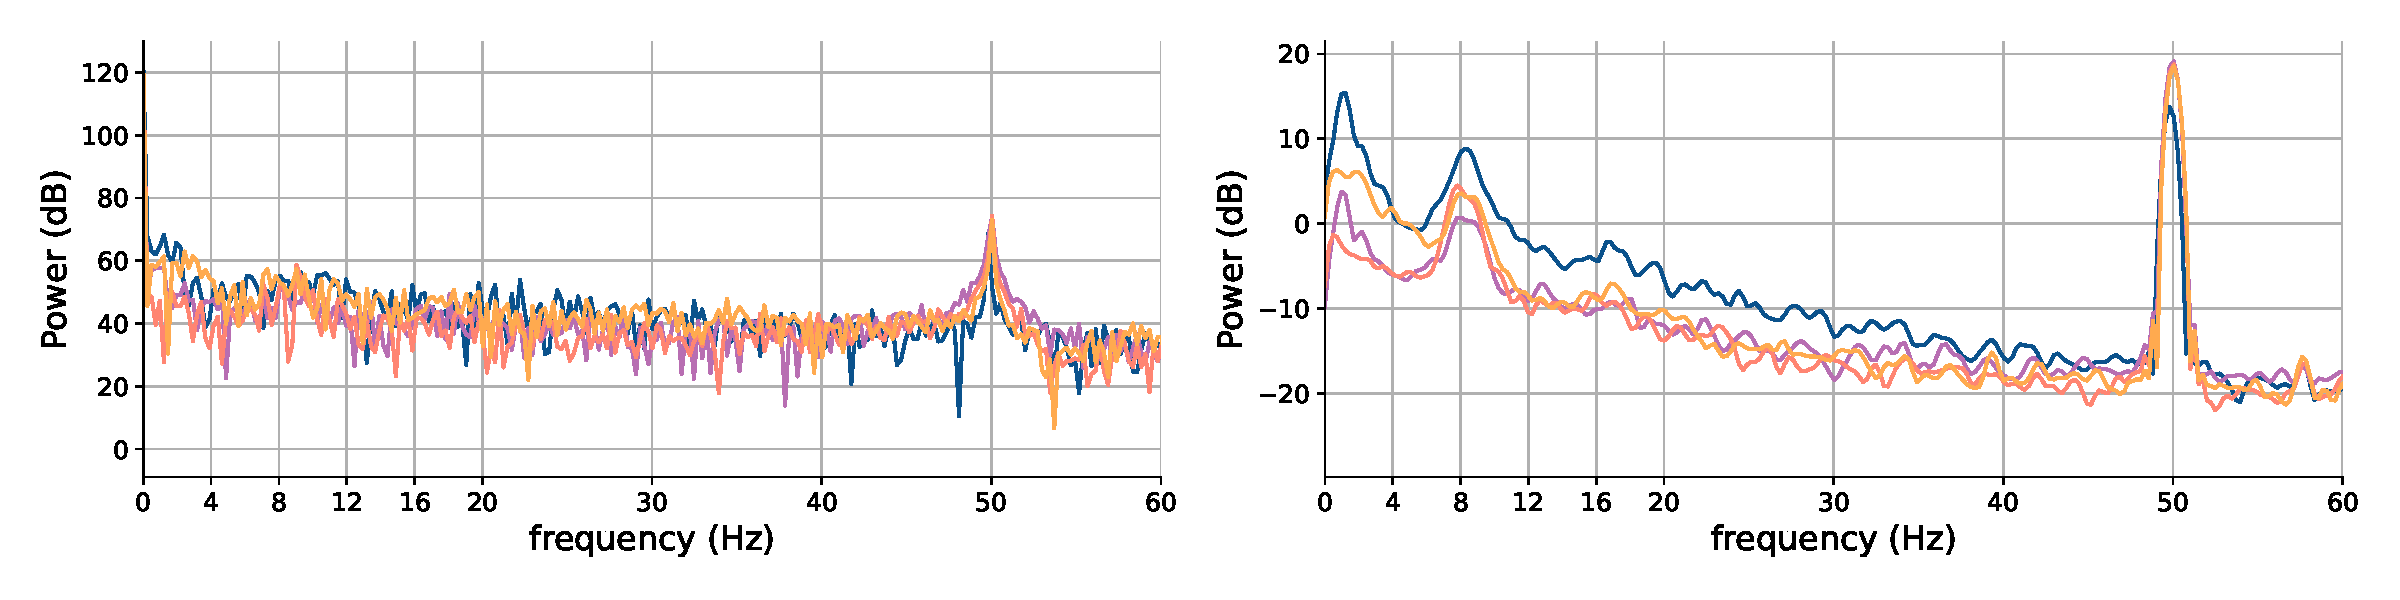
\includegraphics[clip,width=\columnwidth]{eyes_closed_alpha_spectra_N1024.pdf}%
}
\caption[Alpha band test: periodograms showing $N=1024$ point PSD estimates for EEG signals measured from a subject in two distinct states: with eyes open and eyes closed.]{\textbf{Alpha band test}: periodograms showing $N=1024$ point PSD estimates for EEG signals measured from a subject in two distinct states: with eyes open and eyes closed. Data was acquired using the early hardware prototype in Figure \ref{fig:frakenstein-hardware}. Attention should be given to signal power around $8-10$Hz (alpha band). In both (a) and (b), the left subplot shows a standard, non-windowed periodogram accompanied by a Welch-averaged periodogram to the right. Different coloured traces represent independent trials.}
\end{figure}


\section{Experimental Decoding Results}

%% Experiments with varying Nt: GCCA
\begin{figure}[htp]
\subfloat[$T = 0.75$s ($N_s=192, N_s'=48$)]{%
    \label{subfig:gcca-nt-ns48}
    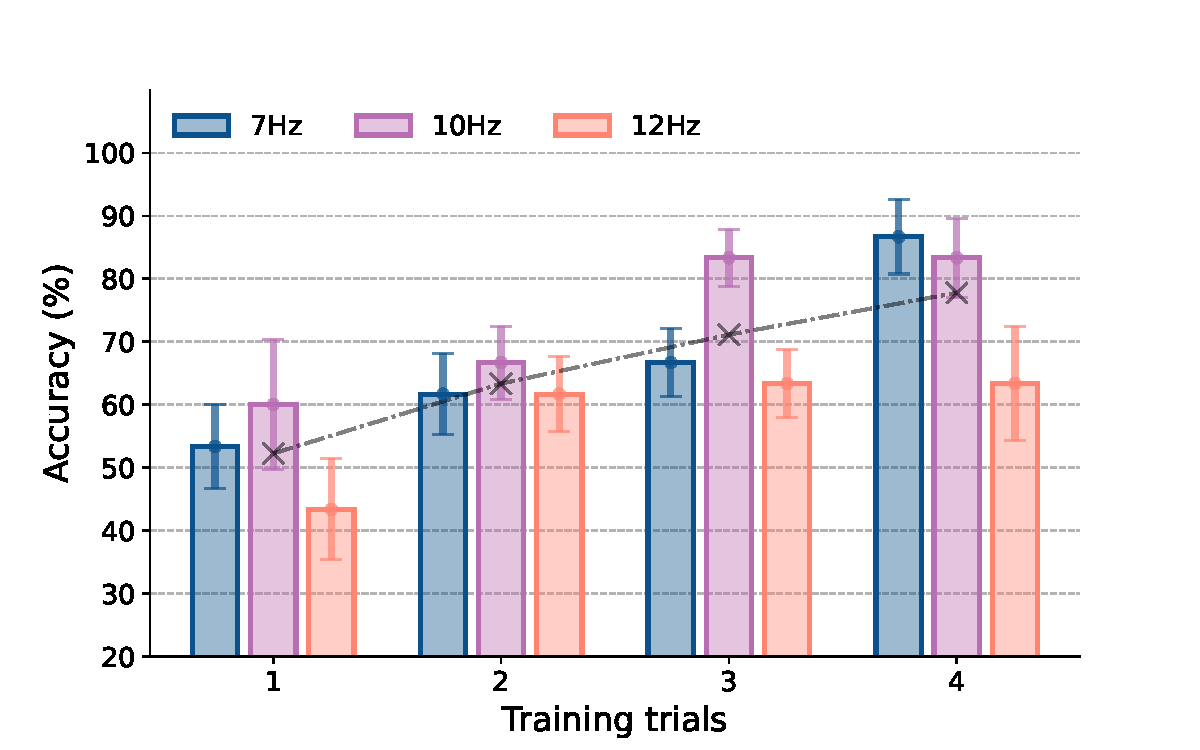
\includegraphics[clip,width=0.49\columnwidth]{report/C6 Results/assets/acc_Nt_gcca_Ns48.pdf}%
    \label{subfig:gcca-nt-ns64}
}
\hfill
\subfloat[$T = 1$s ($N_s=256, N_s'=64$)]{%
    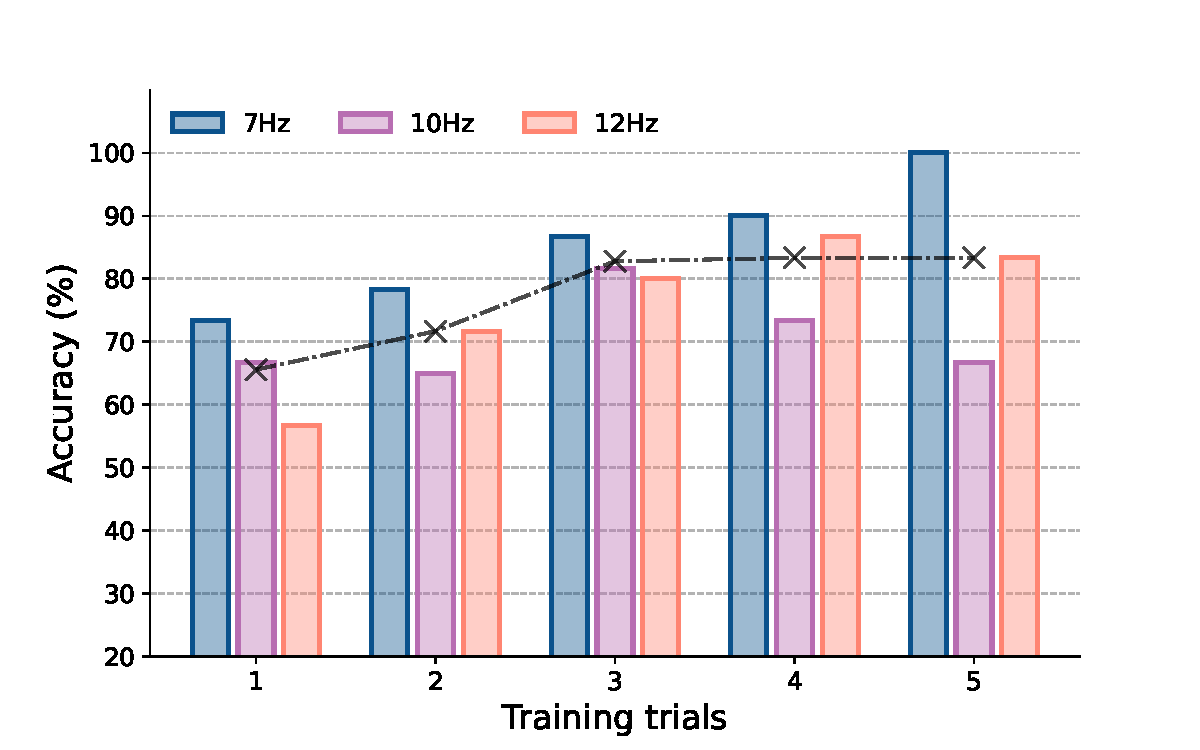
\includegraphics[clip,width=0.49\columnwidth]{report/C6 Results/assets/acc_Nt_gcca_Ns64.pdf}%
    \label{subfig:gcca-nt-ns64}
}
% ensure there is a space below here!

\subfloat[$T = 2$s ($N_s=512, N_s'=128$)]{%
    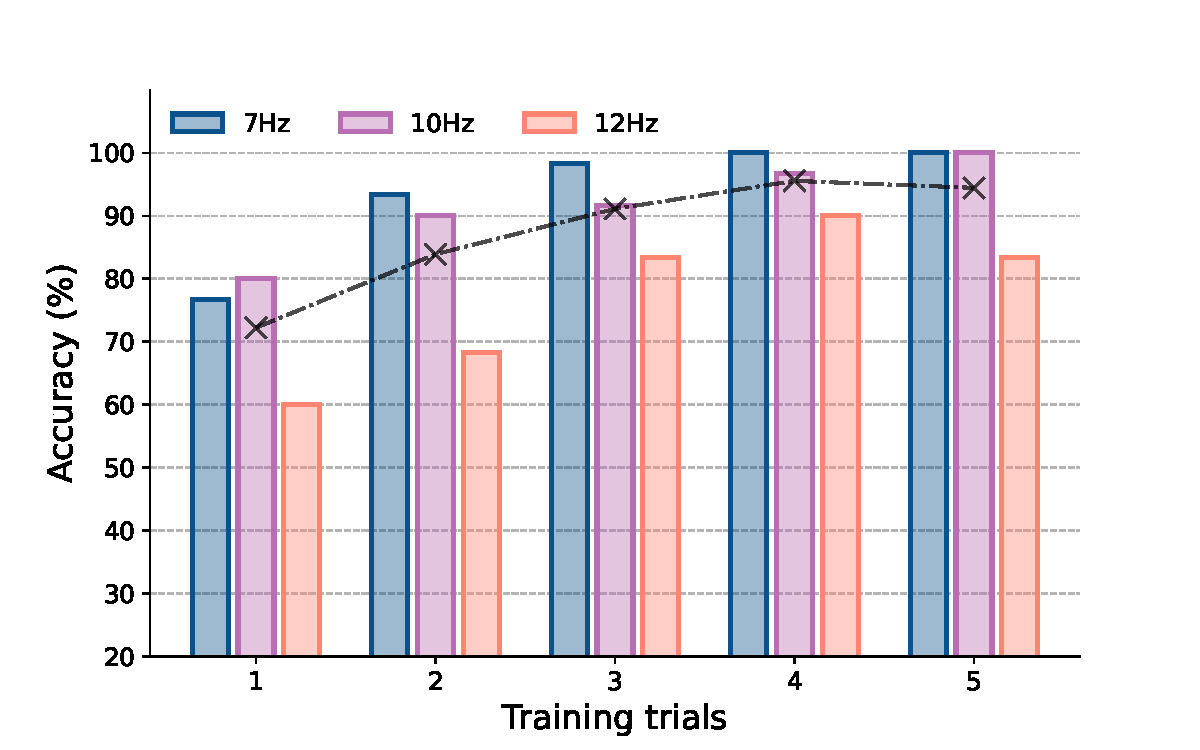
\includegraphics[clip,width=0.49\columnwidth]{report/C6 Results/assets/acc_Nt_gcca_Ns128.pdf}%
    \label{subfig:gcca-nt-ns128}
}
\hfill
\subfloat[$T = 4$s ($N_s=1024, N_s'=256$)]{%
    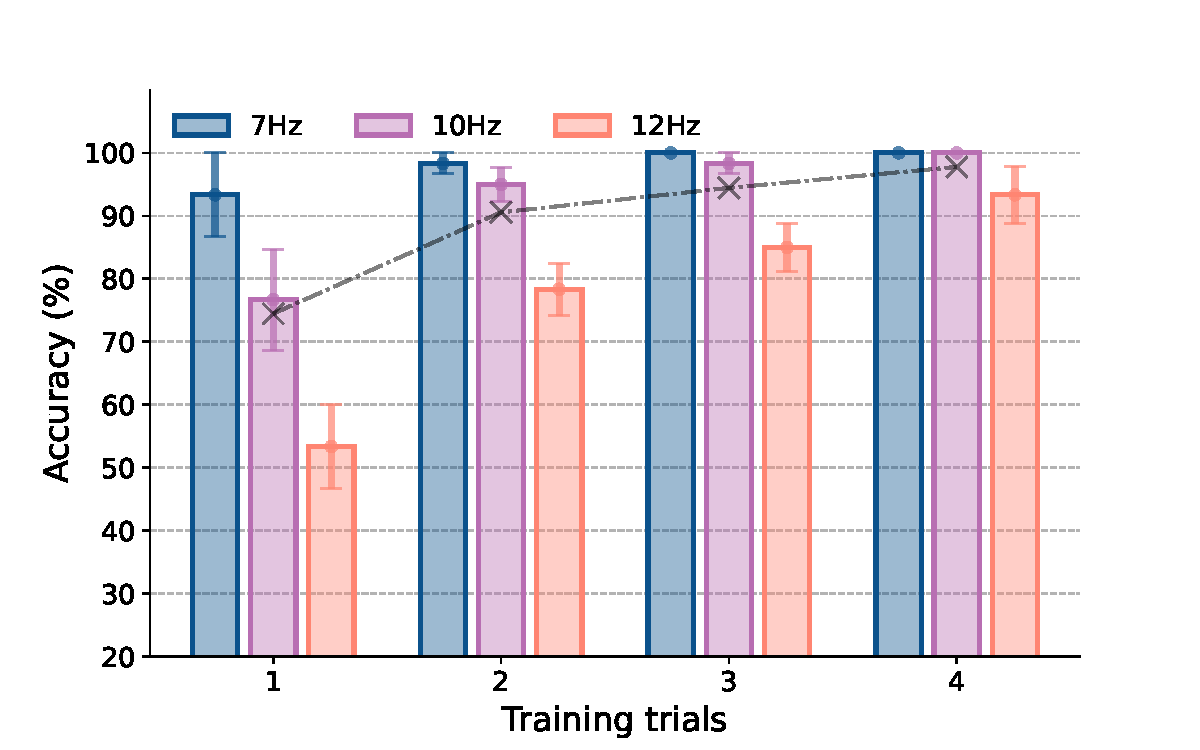
\includegraphics[clip,width=0.49\columnwidth]{report/C6 Results/assets/acc_Nt_gcca_Ns256.pdf}%
    \label{subfig:gcca-nt-ns256}
}

\caption[GCCA decoding accuracy: effect of varying the number of training (calibration) trials $N_t$ on validation accuracy for recording windows of varying length $T$.]{\textbf{GCCA decoding accuracy}: effect of varying the number of training (calibration) trials $N_t$ on validation accuracy for recording windows of varying length $T$. In each subfigure, all trials are of equal length $T$ seconds which equates to $N_s$ samples at $f_s=256$Hz and $N_s'$ samples at the downsampled rate of $f_s'=64$Hz. Crosses connected with dashed traces denote average decoding accuracy across stimulus frequencies for a given $N_t=n, \, n\in\{1, \dots, 5\}$.}
\label{fig:gcca-acc-nt}
\end{figure}


%% Experiments with varying Nt: MsetCCA
\begin{figure}[htp]
\subfloat[$T = 0.75$s ($N_s=192, N_s'=48$)]{%
    \label{subfig:gcca-nt-ns48}
    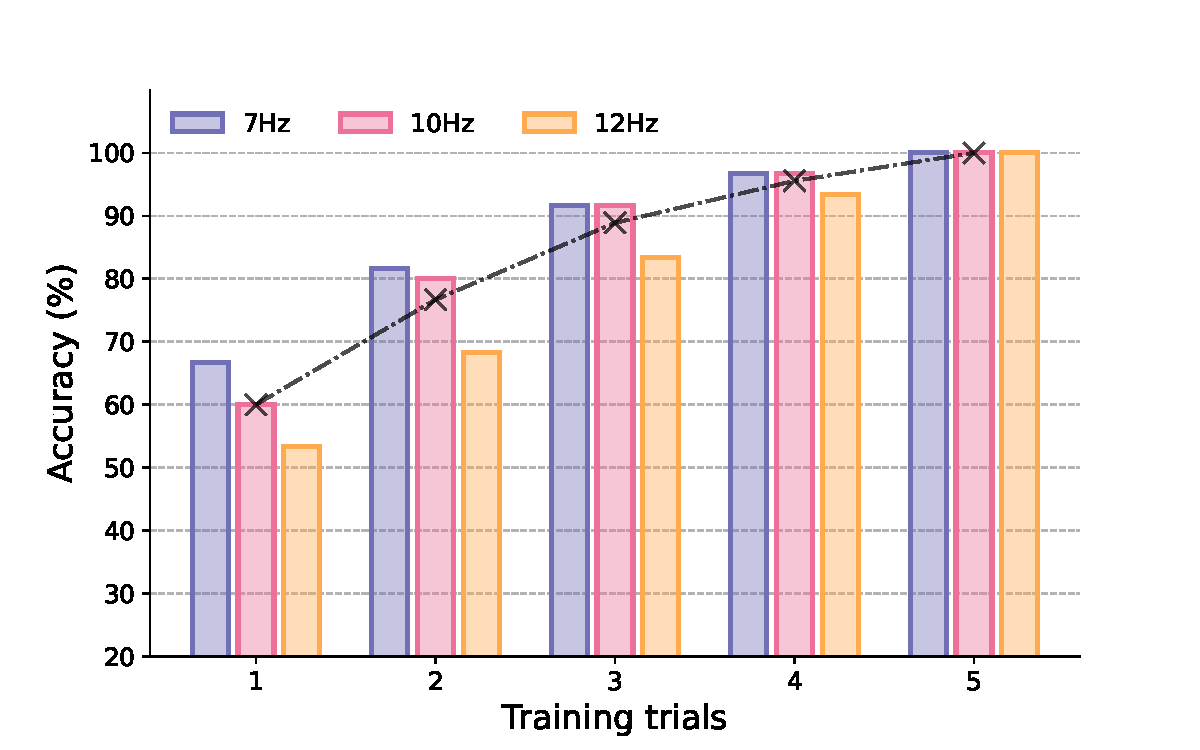
\includegraphics[clip,width=0.49\columnwidth]{report/C6 Results/assets/acc_Nt_mcca_Ns48.pdf}%
}
\hfill
\subfloat[$T = 1$s ($N_s=256, N_s'=64$)]{%
    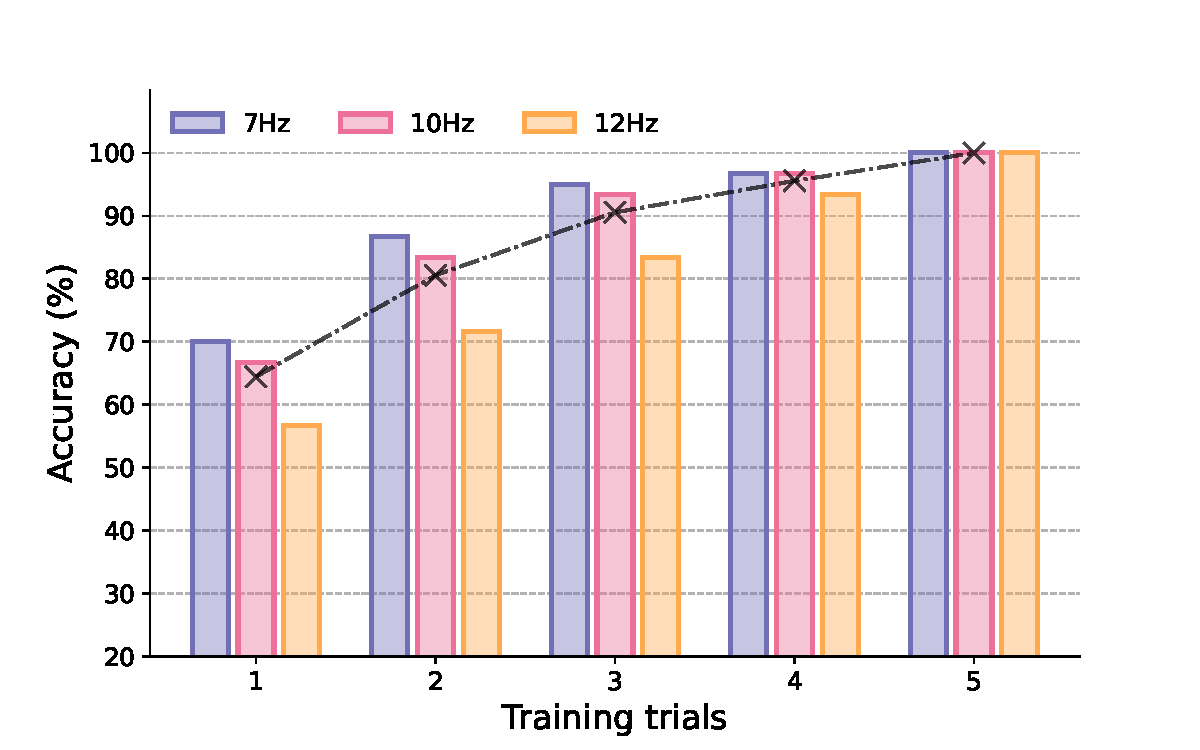
\includegraphics[clip,width=0.49\columnwidth]{report/C6 Results/assets/acc_Nt_mcca_Ns64.pdf}%
    \label{subfig:mset-nt-ns64}
}
% ensure there is a space below here!

\subfloat[$T = 2$s ($N_s=512, N_s'=128$)]{%
    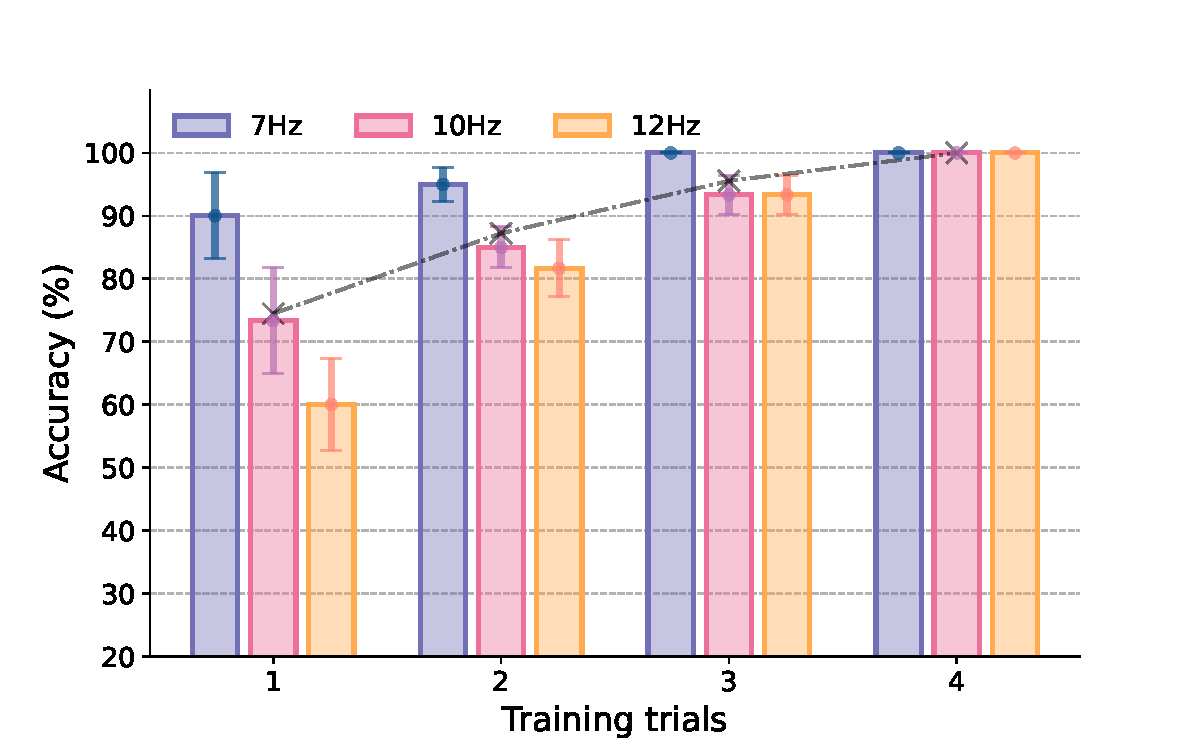
\includegraphics[clip,width=0.49\columnwidth]{report/C6 Results/assets/acc_Nt_mcca_Ns128.pdf}%
    \label{subfig:mset-nt-ns128}
}
\hfill
\subfloat[$T = 4$s ($N_s=1024, N_s'=256$)]{%
    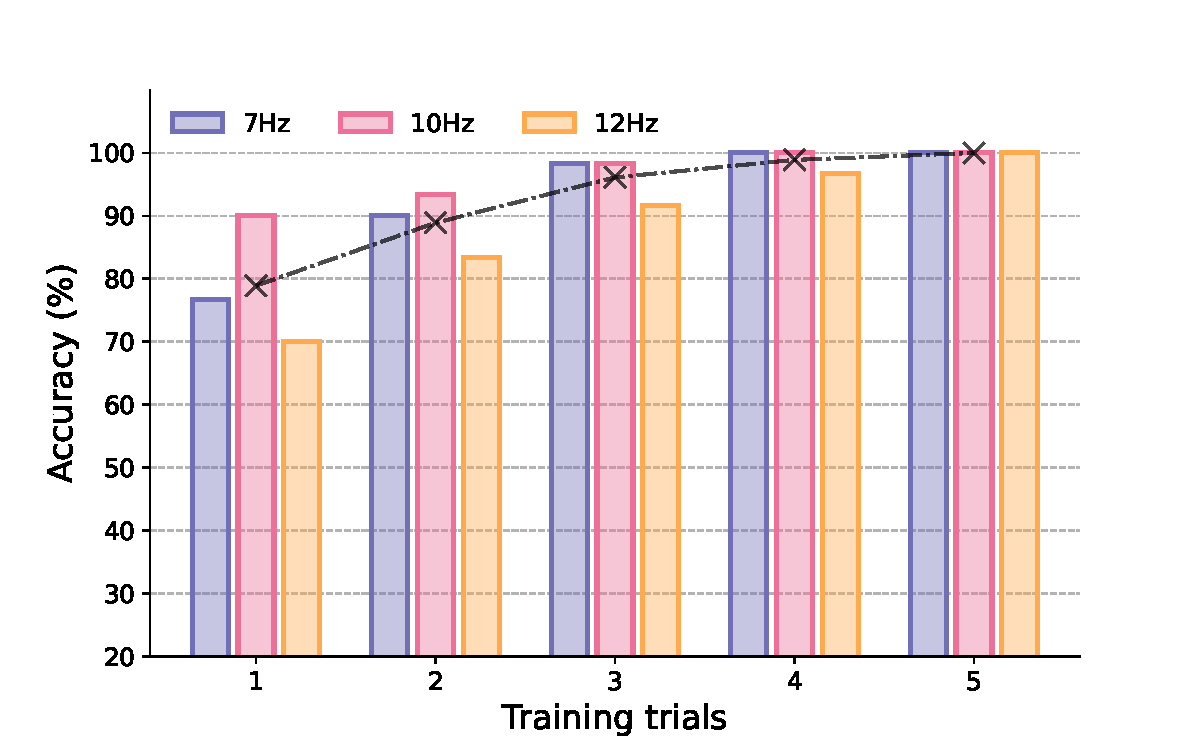
\includegraphics[clip,width=0.49\columnwidth]{report/C6 Results/assets/acc_Nt_mcca_Ns256.pdf}%
    \label{subfig:mset-nt-ns256}
}

\caption[MsetCCA decoding accuracy: effect of varying the number of training (calibration) trials $N_t$ on validation accuracy for recording windows of varying length $T$.]{\textbf{MsetCCA decoding accuracy}: effect of varying the number of training (calibration) trials $N_t$ on validation accuracy for recording windows of varying length $T$. In each subfigure, all trials are of equal length $T$ seconds which equates to $N_s$ samples at $f_s=256$Hz and $N_s'$ samples at the downsampled rate of $f_s'=64$Hz. Crosses connected with dashed traces denote average decoding accuracy across stimulus frequencies for a given $N_t=n, \, n\in\{1, \dots, 5\}$.}
\label{fig:mset-acc-nt}
\end{figure}

%% [SAMPLING LENGTH] Experiments with varying Ns: GCCA
\begin{figure}[htp]
\subfloat[$N_t=1$]{%
    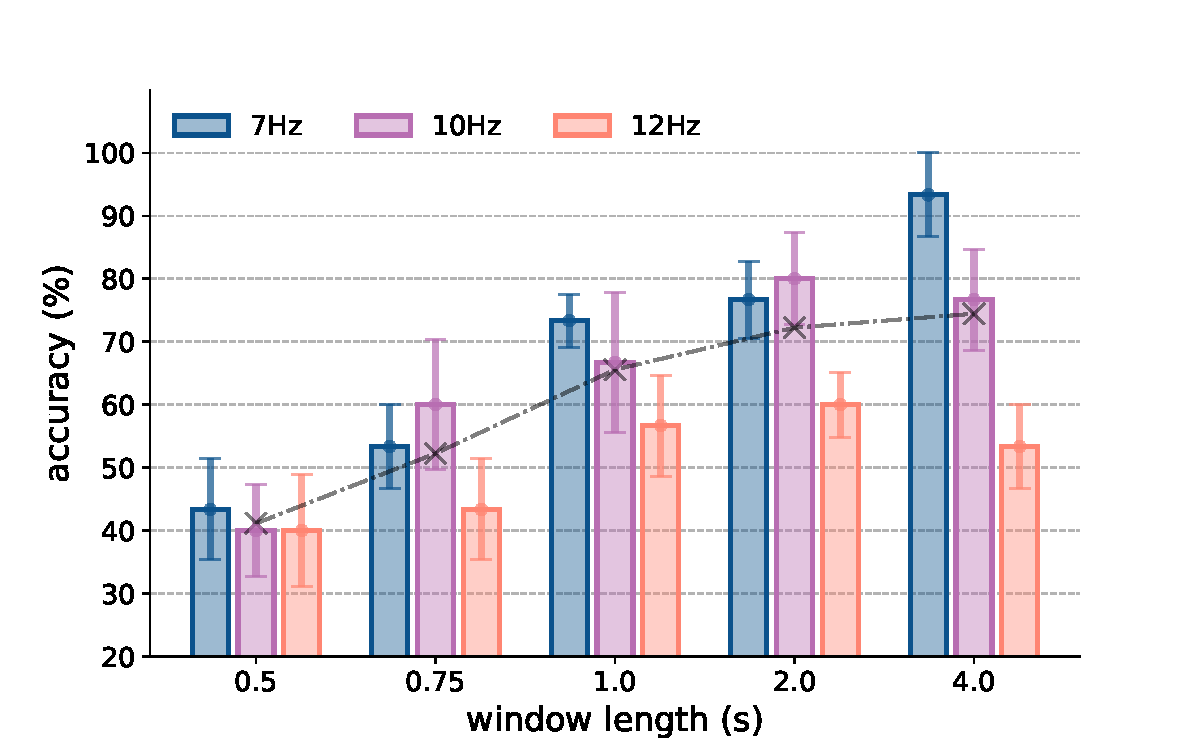
\includegraphics[clip,width=0.49\columnwidth]{report/C6 Results/assets/acc_Ns_gcca_Nt1.pdf}%
    \label{subfig:gcca-ns-nt1}
}
\hfill
\subfloat[$N_t=2$]{%
    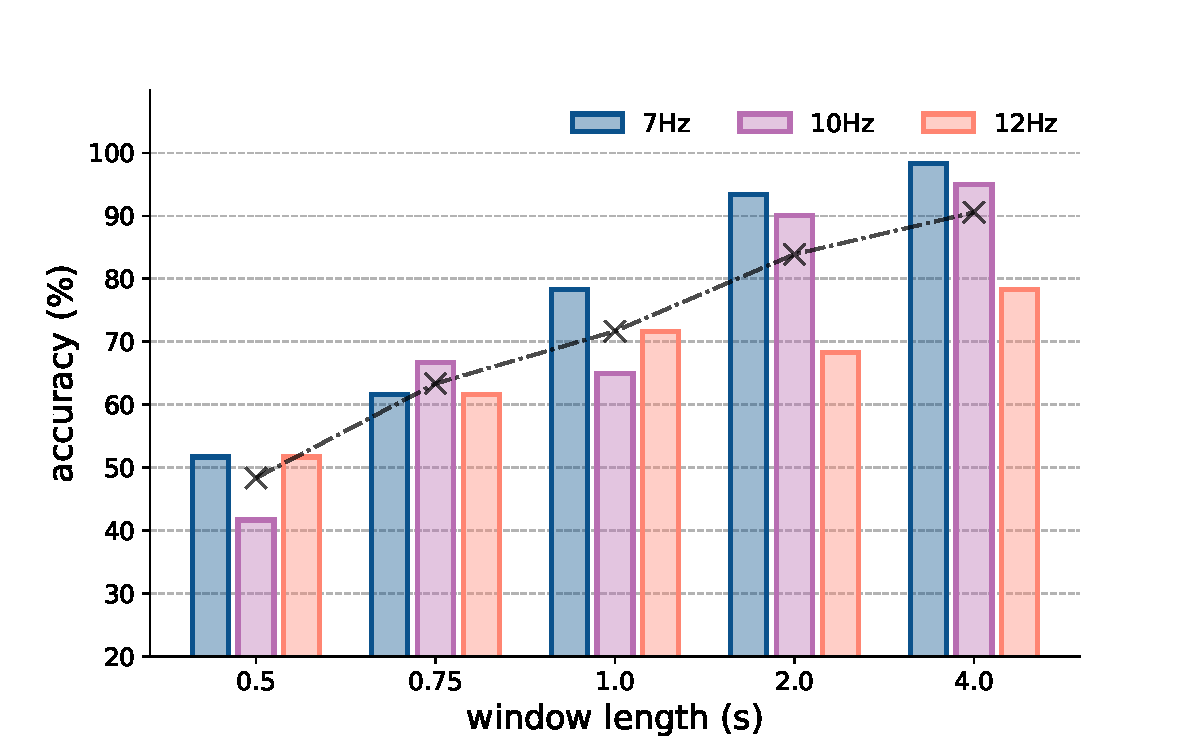
\includegraphics[clip,width=0.49\columnwidth]{report/C6 Results/assets/acc_Ns_gcca_Nt2.pdf}%
    \label{subfig:gcca-ns-nt2}
}
% ensure there is a space below here!

\subfloat[$N_t=3$)]{%
    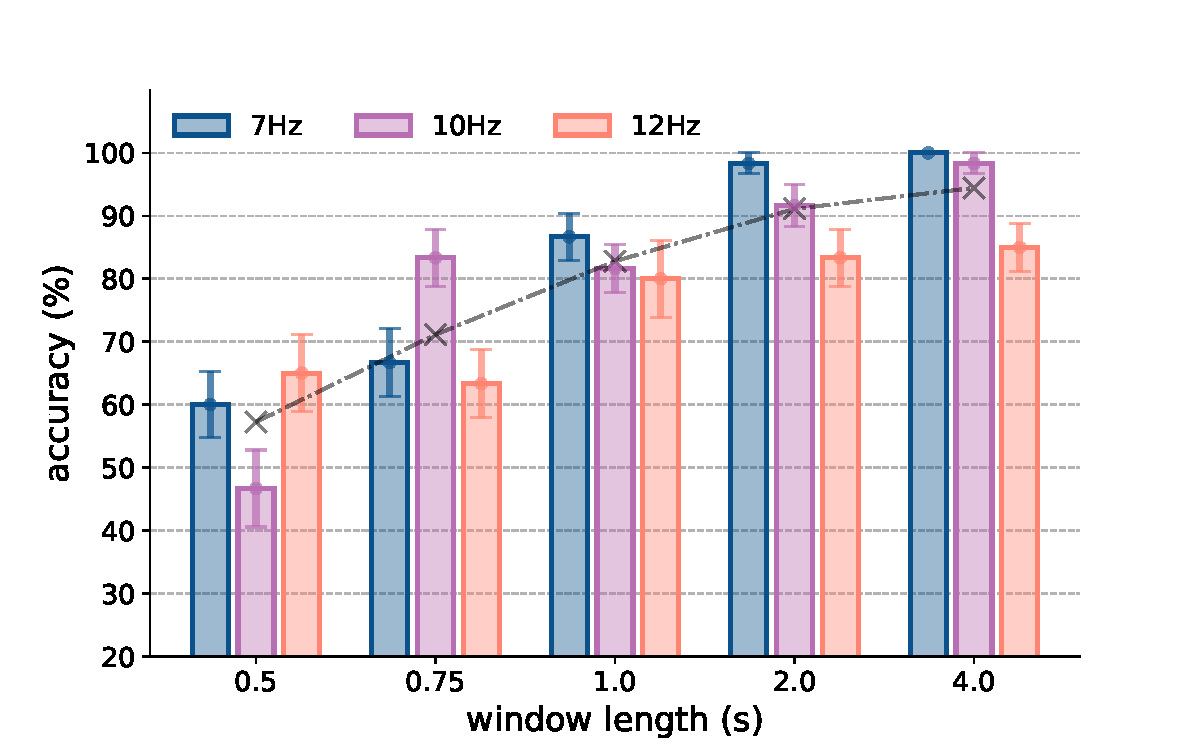
\includegraphics[clip,width=0.49\columnwidth]{report/C6 Results/assets/acc_Ns_gcca_Nt3.pdf}%
    \label{subfig:gcca-ns-nt3}
}
\hfill
\subfloat[$N_t=4$]{%
    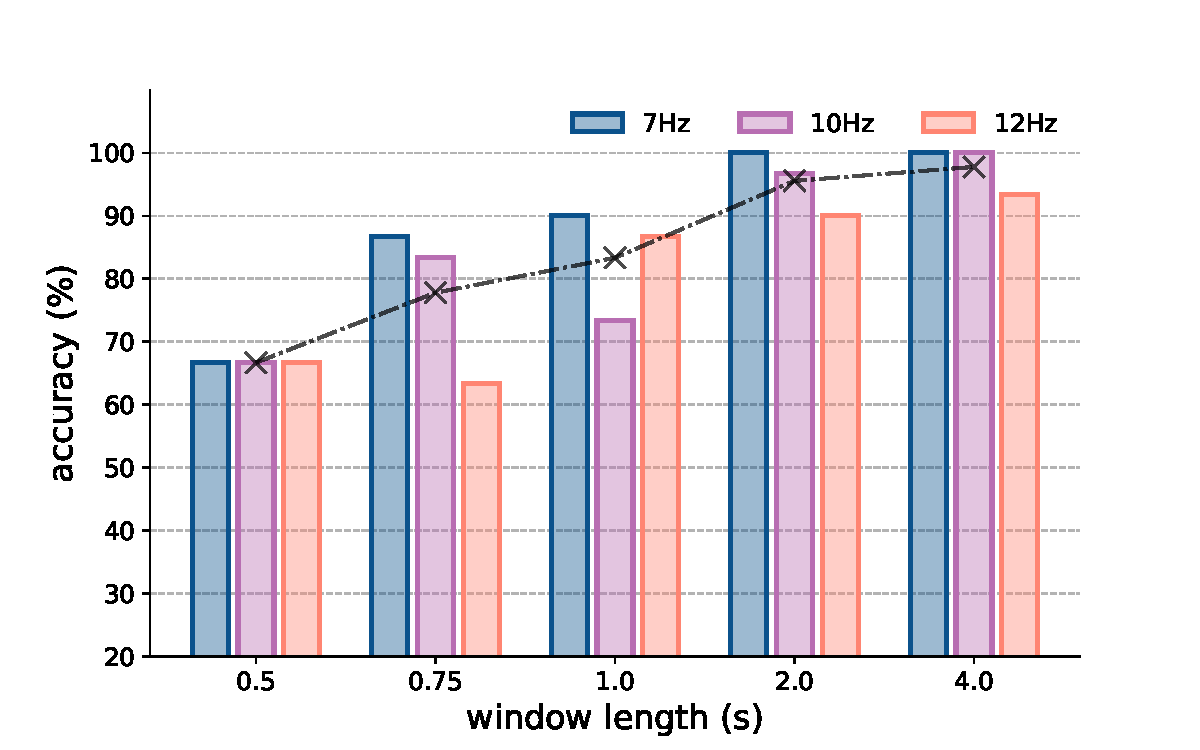
\includegraphics[clip,width=0.49\columnwidth]{report/C6 Results/assets/acc_Ns_gcca_Nt4.pdf}%
    \label{subfig:gcca-ns-nt4}
}

\caption[GCCA decoding accuracy: effect of varying recording window length $T$ on validation accuracy for different numbers of calibration trails $N_t$]{\textbf{GCCA decoding accuracy}: effect of varying recording window length $T$ on validation accuracy for different numbers of calibration trails $N_t$. In each subfigure, all results were computed using $N_t=n, \, n\in\{1, \dots, 4\}$ calibration trials. Crosses connected with dashed traces denote average decoding accuracy across stimulus frequencies for a given a given window length $T$.}
\label{fig:gcca-acc-ns}
\end{figure}

%% [SAMPLING LENGTH] Experiments with varying Ns: MsetCCA
\begin{figure}[htp]
\subfloat[$N_t=1$]{%
    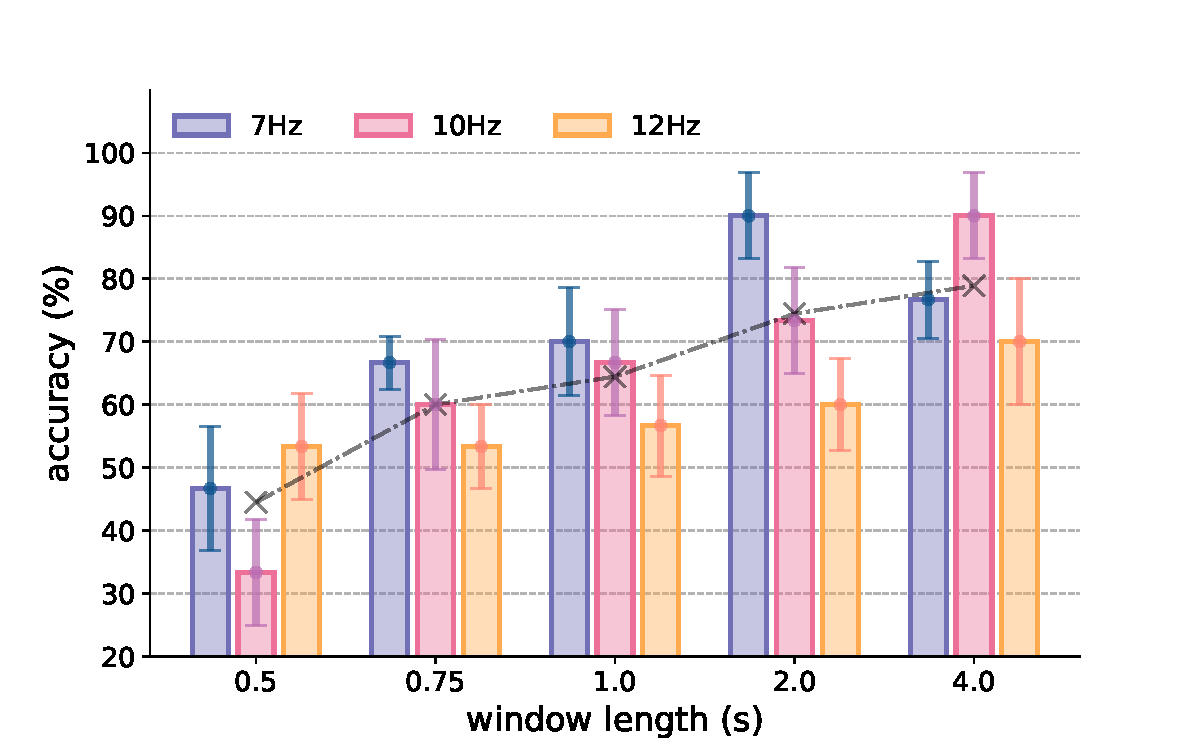
\includegraphics[clip,width=0.49\columnwidth]{report/C6 Results/assets/acc_Ns_mcca_Nt1.pdf}%
    \label{subfig:mcca-ns-nt1}
}
\hfill
\subfloat[$N_t=2$]{%
    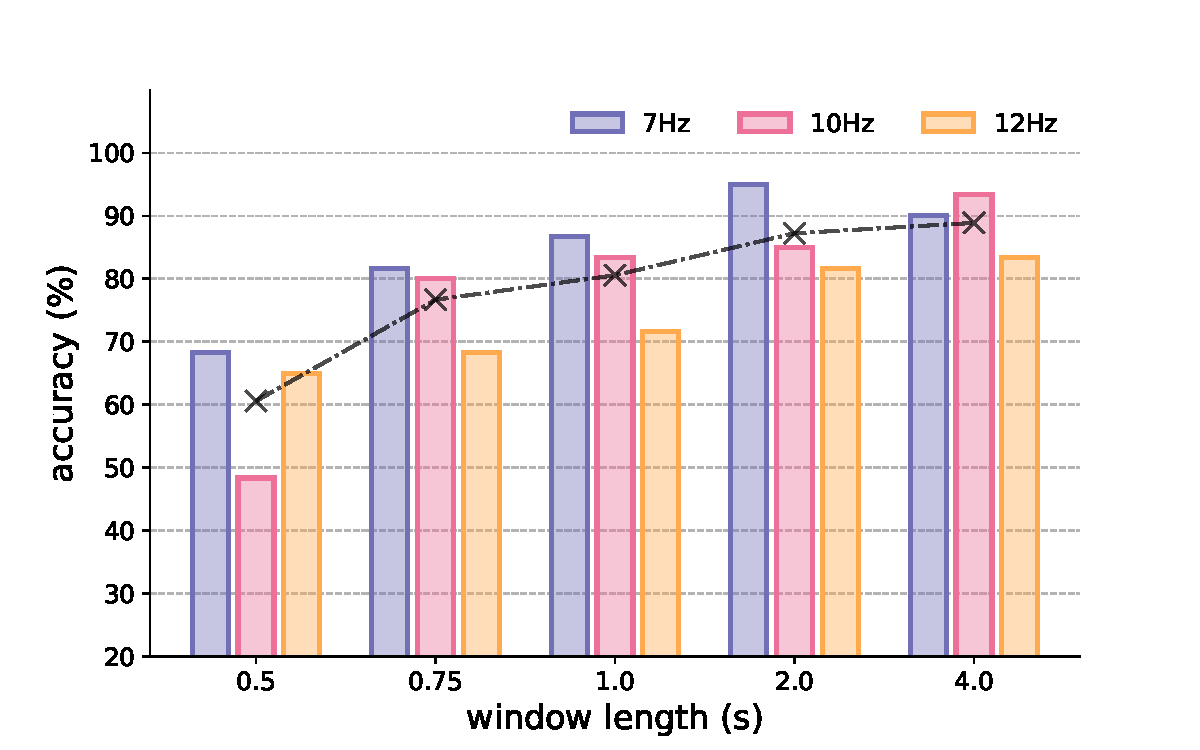
\includegraphics[clip,width=0.49\columnwidth]{report/C6 Results/assets/acc_Ns_mcca_Nt2.pdf}%
    \label{subfig:mcca-ns-nt2}
}
% ensure there is a space below here!

\subfloat[$N_t=3$)]{%
    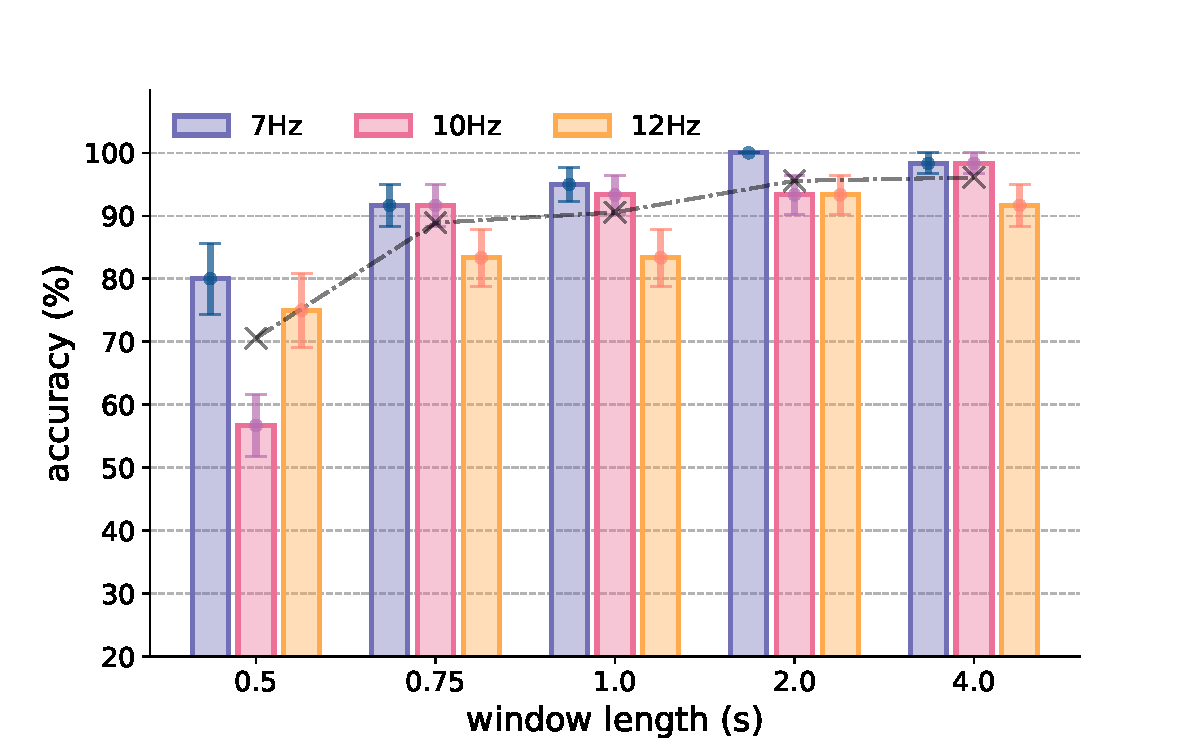
\includegraphics[clip,width=0.49\columnwidth]{report/C6 Results/assets/acc_Ns_mcca_Nt3.pdf}%
    \label{subfig:mcca-ns-nt3}
}
\hfill
\subfloat[$N_t=4$]{%
    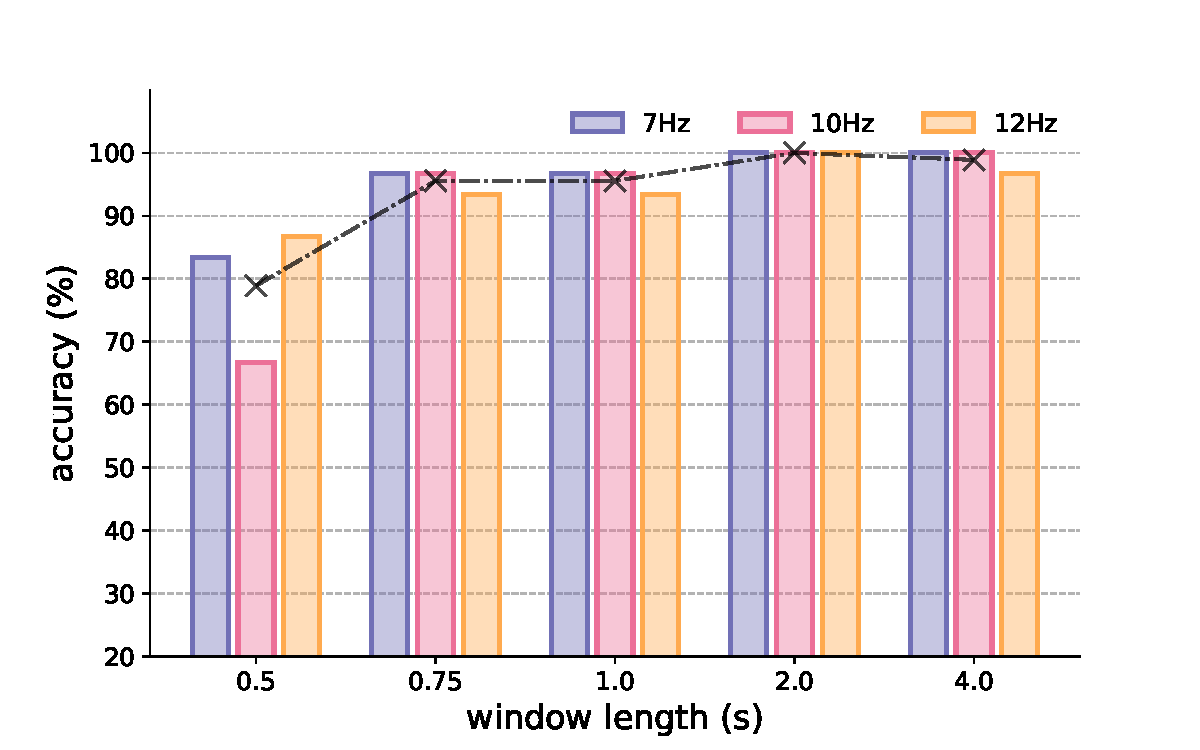
\includegraphics[clip,width=0.49\columnwidth]{report/C6 Results/assets/acc_Ns_mcca_Nt4.pdf}%
    \label{subfig:mcca-ns-nt4}
}

\caption[MsetCCA decoding accuracy: effect of varying recording window length $T$ on validation accuracy for different numbers of calibration trails $N_t$]{\textbf{MsetCCA decoding accuracy}: effect of varying recording window length $T$ on validation accuracy for different numbers of calibration trails $N_t$. In each subfigure, all results were computed using $N_t=n, \, n\in\{1, \dots, 4\}$ calibration trials. Crosses connected with dashed traces denote average decoding accuracy across stimulus frequencies for a given a given window length $T$.}
\label{fig:mcca-acc-ns}
\end{figure}

% \begin{figure}
%      \centering
%      \begin{subfigure}[b]{0.3\textwidth}
%          \centering
%          \includegraphics[width=\textwidth]{acc}
%          \caption{$y=x$}
%          \label{fig:y equals x}
%      \end{subfigure}
%      \hfill
%      \begin{subfigure}[b]{0.3\textwidth}
%          \centering
%          \includegraphics[width=\textwidth]{graph2}
%          \caption{$y=3sinx$}
%          \label{fig:three sin x}
%      \end{subfigure}
%      \hfill
%      \begin{subfigure}[b]{0.3\textwidth}
%          \centering
%          \includegraphics[width=\textwidth]{graph3}
%          \caption{$y=5/x$}
%          \label{fig:five over x}
%      \end{subfigure}
%         \caption{Three simple graphs}
%         \label{fig:three graphs}
% \end{figure}

% \section{Experiments using Benchmark Data}


%% Chapter 7: Discussion and Conclusion
%% Chapter 7: Discussion and Conclusion
\chapter{Discussion and Conclusion}
\label{chapter:discussion-conclusion}

\graphicspath{ {report/Chapter7/assets/} } 

\section{Discussion}
Lessons learnt

\subsection{Challenges encountered}
Discuss numerical challenges, precision issues, memory constraints
Discuss some of the auxiliary computational approaches used such as eigenvalue solvers etc

Mention how most other reports like MsetCCA and GCCA compare effect of following on acc:
- number of harmonics 
- number of channels
obv not possible in this project.

Mention somewhere that the networking aspect with MQTT can stream data up to 5Hz but was only required to do so at around 1Hz (2s sampling window with 50\% overlap)



\section{Conclusion and Future Work}
Evaluate if objectives initially laid out were achieved
- if not, why not
- if they had been stated differently/more realistically, would the outcome have been different?
- what would need to be done differently next time


% Chapter 4: Experimental Procedure 
\chapter{Appendices}
\label{chapter:appendices}

\graphicspath{ {report/Appendices/assets/} } 

% \setlength{\voffset}{0cm}
% \setlength{\hoffset}{0cm}

\section{Firmware Implementations}
\label{app:firmware}

\begin{listing}[!htb]
\footnotesize
\begin{minted}{python}
from ulab import numpy as np

def power_iteration(A, iterations):
    """
    Iterative algo. to find the eigenvector of a matrix A corresponding to the largest
    eigenvalue.
    """
    # choose random initial vector to reduce risk of choosing one orthogonal to 
    # target eigen vector
    b_k = np.array([urandom.random() for i in range(len(A))])

    for _ in range(iterations):
        b_k1 = np.dot(A, b_k)
        b_k1_norm = np.linalg.norm(b_k1)
        # re normalize the vector
        b_k = b_k1 / b_k1_norm

    return b_k1_norm, b_k

\end{minted}
\caption{MicroPython implementation of the Power Iteration algorithm presented in Algorithm \ref{alg:power-iteration} for finding the maximum real eigenvalue of a symmetric, real-valued matrix}
\label{app-listing:power-iteration-mpy}
\end{listing}

\begin{listing}[!htb]
\footnotesize
\begin{minted}{python}
from ulab import numpy as np

def qr_iteration(A, iterations=30):
    
    """
    Use the QR iteration algorithm to iteratively solve for the eigenvectors and eigenvalues
    of a matrix A. Note: only guaranteed to recover exactly for symmetric matrices
    with real eigenvalues. May work partially for asymmetric matrices (no complex support yet).
    
    Number of iterations is specified by `iterations` and should be tuned empirically. Typically,
    30 is more than enough.
    Returns:
        `lam`: vector of eigenvalues
        `Q_bar`: matrix of eigenvectors (columns)
    """

    Ak = A
    Q_bar = np.eye(len(Ak))

    for _ in range(iterations):
        Qk, Rk = np.linalg.qr(Ak)
        Ak = np.dot(Rk, Qk)
        Q_bar = np.dot(Q_bar, Qk)

    lam = np.diag(Ak)
    return lam, Q_bar

\end{minted}
\caption{MicroPython implementation of the QR Iteration algorithm presented in Algorithm \ref{alg:qr-iteration}}
\label{app-listing:qr-iteration-mpy}
\end{listing}

\begin{listing}[h]
\footnotesize
\begin{minted}{python}
from ulab import numpy as np

def solve_gen_eig_prob(A, B, eps=1e-6):
    """
    Solves the generalised eigenvalue problem of the form:
    Aw = lambda*Bw
    
    Note: can be validated against `scipy.linalg.eig(A, b=B)`
    
    Ref: 
    'Eigenvalue and Generalized Eigenvalue Problems: Tutorial (2019)'
    Benyamin Ghojogh and Fakhri Karray and Mark Crowley
    arXiv 1903.11240

    """
    Lam_b, Phi_b = np.linalg.eig(B) # eig decomp of B alone
    Lam_b = np.eye(len(Lam_b))*Lam_b # convert to diagonal matrix of eig vals
    
    Lam_b_sq = replace_nan(Lam_b**0.5)+np.eye(len(Lam_b))*eps
    Phi_b_hat = np.dot(Phi_b, np.linalg.inv(Lam_b_sq))
    A_hat = np.dot(np.dot(Phi_b_hat.transpose(), A), Phi_b_hat)
    Lam_a, Phi_a = np.linalg.eig(A_hat)
    Lam_a = np.eye(len(Lam_a))*Lam_a
    
    Lam = Lam_a
    Phi = np.dot(Phi_b_hat, Phi_a)
    
    return np.diag(Lam), Phi

\end{minted}
\caption{MicroPython implementation of the generalised eigenvalue algorithm in Algorithm \ref{alg:gen-eig-algo}}
\label{app-listing:gen-eig-prob-mpy}
\end{listing}

\begin{listing}[h]
\footnotesize
\begin{minted}{python}
from ulab import numpy as np

class CCA():
    """
    Canonical Correlation Analysis algorithm for SSVEP decoding. Reference 
    signal `Y` is a harmonic reference set with `Nh` harmonics.
    
    Expects a list of `stim_freqs` corresponding to SSVEP stimulus frequencies.
    Requires sampling frequncy `fs` for the harmonic ref.
    """
    
    def __init__(self, stim_freqs, fs, Nh=2):
        self.Nh = Nh
        self.stim_freqs = stim_freqs
        self.fs = fs
        
    def compute_corr(self, X_test):            
        result = {}
        Cxx = np.dot(X_test, X_test.transpose()) # precompute data auto correlation matrix
        for f in self.stim_freqs:
            Y = harmonic_reference(f, self.fs, np.max(X_test.shape), Nh=self.Nh, standardise_out=False)
            rho = self.cca_eig(X_test, Y, Cxx=Cxx) # canonical variable matrices. Xc = X^T.W_x
            result[f] = rho
        return result
    
    @staticmethod # define as static to allow non-CCA instances to use this func
    def cca_eig(X, Y, Cxx=None, eps=1e-6):
        if Cxx is None:
            Cxx = np.dot(X, X.transpose()) # signal covariance matrix
        Cyy = np.dot(Y, Y.transpose())  # reference covariance matrix
        Cxy = np.dot(X, Y.transpose()) # cross covariance matrix
        Cyx = np.dot(Y, X.transpose()) # same as Cxy.T

        M1 = np.dot(np.linalg.inv(Cxx+eps), Cxy) # intermediate result
        M2 = np.dot(np.linalg.inv(Cyy+eps), Cyx)

        lam, _ = solve_eig_qr(np.dot(M1, M2), 20) # solve eig. vals using QR iteration
        return np.sqrt(lam)

\end{minted}
\caption{MicroPython implementation of the CCA algorithm from Algorithm \ref{alg:cca}}
\label{app-listing:cca-algo}
\end{listing}

\begin{listing}[h]
\footnotesize
\begin{minted}{python}
from ulab import numpy as np

class UnivariateMsetCCA():
    """
    Multiset CCA algorithm for SSVEP decoding.
    
    Computes optimised reference signal set based on historical observations
    and uses ordinary CCA for final correlation computation given a new test
    signal.
    
    Note: this is a 1 channel implementation (Nc=1)
    """
    
    def __init__(self):
        self.Ns, self.Nt = None, None
        
    def fit(self, X, compress_ref=True):
        """
        Expects a training matrix X of shape Nt x Ns. If `compress_ref=True`, the `Nt` components
        in optimised reference signal Y will be averaged to form a single reference vector. This
        can be used for memory optimisation but will likely degrade performance slightly.         
        """
        if X.shape[0] > X.shape[1]:
            print("Warning: received more trials than samples. This is unusual behaviour: check X")
        R = np.dot(X, X.transpose()) # inter trial covariance matrix
        S = np.eye(len(R))*np.diag(R) # intra-trial diag covariance matrix

        lam, V = solve_gen_eig_prob((R-S), S) # solve generalised eig problem
        w = V[:, np.argmax(lam)] # find eigenvector corresp to largest eigenvalue
        Y = np.array([x*w[i] for i, x in enumerate(X)]) # store optimised reference vector Nt x Ns
        self.Y  = Y
        if compress_ref:
            self.Y = np.mean(Y, axis=0).reshape((1, max(Y.shape))) # this will average Nt components in Y: Nc x Nt -> 1 x Nt
        
    def compute(self, X_test):
        if self.Y is None:
            raise ValueError("Reference matrix Y must be computed using `fit` before computing corr")
        if len(X_test.shape) == 1:
            X_test = X_test.reshape((1, len(X_test)))
        return CCA.cca_eig(X_test, self.Y)[0] # use ordinary CCA with optimised ref. Y

\end{minted}
\caption{MicroPython implementation of the MsetCCA algorithm from Algorithm \ref{alg:mset-cca}}
\label{app-listing:mcca-algo}
\end{listing}

\begin{listing}[h]
\footnotesize
\begin{minted}{python}
from ulab import numpy as np

class GCCA():
    """
    Generalised canonical component analysis.
    
    Expects the target frequency at `f_ssvep`. `fs` is the sampling rate used and `Nh` the number of harmonics for the harmonic reference signal. 
    
    Ref: 'Improving SSVEP Identification Accuracy via Generalized Canonical Correlation Analysis'
    Sun, Chen et al
    """
    
    def __init__(self, f_ssvep, fs, Nh=3, name=None):
        self.Nc, self.Ns, self.Nt = None, None, None
        self.Nh = Nh
        self.w_chi_bar_n = None
        self.w_Y_n = None
        self.w_Chi_n = None
        self.fs = fs
        self.f_ssvep = f_ssvep
        
        self.name = name or "gcca_{0}hz".format(f_ssvep)
            
        
    def fit(self, X):
        """
        Fit against training tensor X.
        
        X should be a 3rd order tensor of dim (Nc x Ns x Nt)
        """
        assert len(X.shape) == 3, "Expected 4th order input data tensor: Nc x Ns x Nt"
        self.Nc, self.Ns, self.Nt = X.shape
        
        Chi_n = X
        Chi_n_c = Chi_n.reshape((self.Nc, self.Ns*self.Nt))

        Chi_bar_n = np.mean(Chi_n, axis=-1) # mean over trials for each channel with all samples: output shape is Nc x Ns x 1
        Chi_bar_n_c = np.concatenate([Chi_bar_n for i in range(self.Nt)], axis=1) # concat along columns

        Y_n = cca_reference([self.f_ssvep], self.fs, self.Ns, Nh=self.Nh).reshape(-1, self.Ns)
        Y_n_c = np.concatenate([Y_n for i in range(self.Nt)], axis=1)

        # form X and D and find eigenvals
        X = np.c_[Chi_n_c.T, Chi_bar_n_c.T, Y_n_c.T].T

        d1 = Chi_n_c.dot(Chi_n_c.T)
        d2 = Chi_bar_n_c.dot(Chi_bar_n_c.T)
        d3 = Y_n_c.dot(Y_n_c.T)
        D = block_diag(d1, d2, d3)

        lam, W_eig = solve_gen_eig_prob(X.dot(X.T), D) # solve generalised eigenvalue problem

        i = np.argmax(np.real(lam))
        w = W_eig[:, i] # optimal spatial filter vector with dim (2*Nc + 2*Nh)
        
        w_Chi_n = w[:self.Nc] # first Nc weight values correspond to data channels
        w_Chi_bar_n = w[self.Nc:2*self.Nc] # second Nc weights correspond to Nc template channels
        w_Y_n = w[2*self.Nc:] # final 2*Nh weights correspond to ref sinusoids with harmonics
        
        self.w_chi_bar_n =  w_Chi_bar_n.T.dot(Chi_bar_n)
        self.w_Y_n = w_Y_n.T.dot(Y_n)
        self.w_Chi_n = w_Chi_n
            
    def compute(self, X_test):
        if self.w_chi_bar_n is None:
            raise ValueError("call `.fit(X_train)` before performing classification.")

        rho1 = correlation(self.w_Chi_n.T.dot(X_test), self.w_chi_bar_n)[0]
        rho2 = correlation(self.w_Chi_n.T.dot(X_test), self.w_Y_n)[0]

        return np.sum([np.sign(rho_i)*rho_i**2 for rho_i in [rho1, rho2]])

\end{minted}
\caption{Python implementation of the GCCA algorithm from Algorithm \ref{alg:gcca}}
\label{app-listing:gcca-algo}
\end{listing}

% \setlength{\voffset}{-2.54cm}
% \setlength{\hoffset}{-2.54cm}

\section{EEG Hardware Schematics}

\label{appendix:schematics}
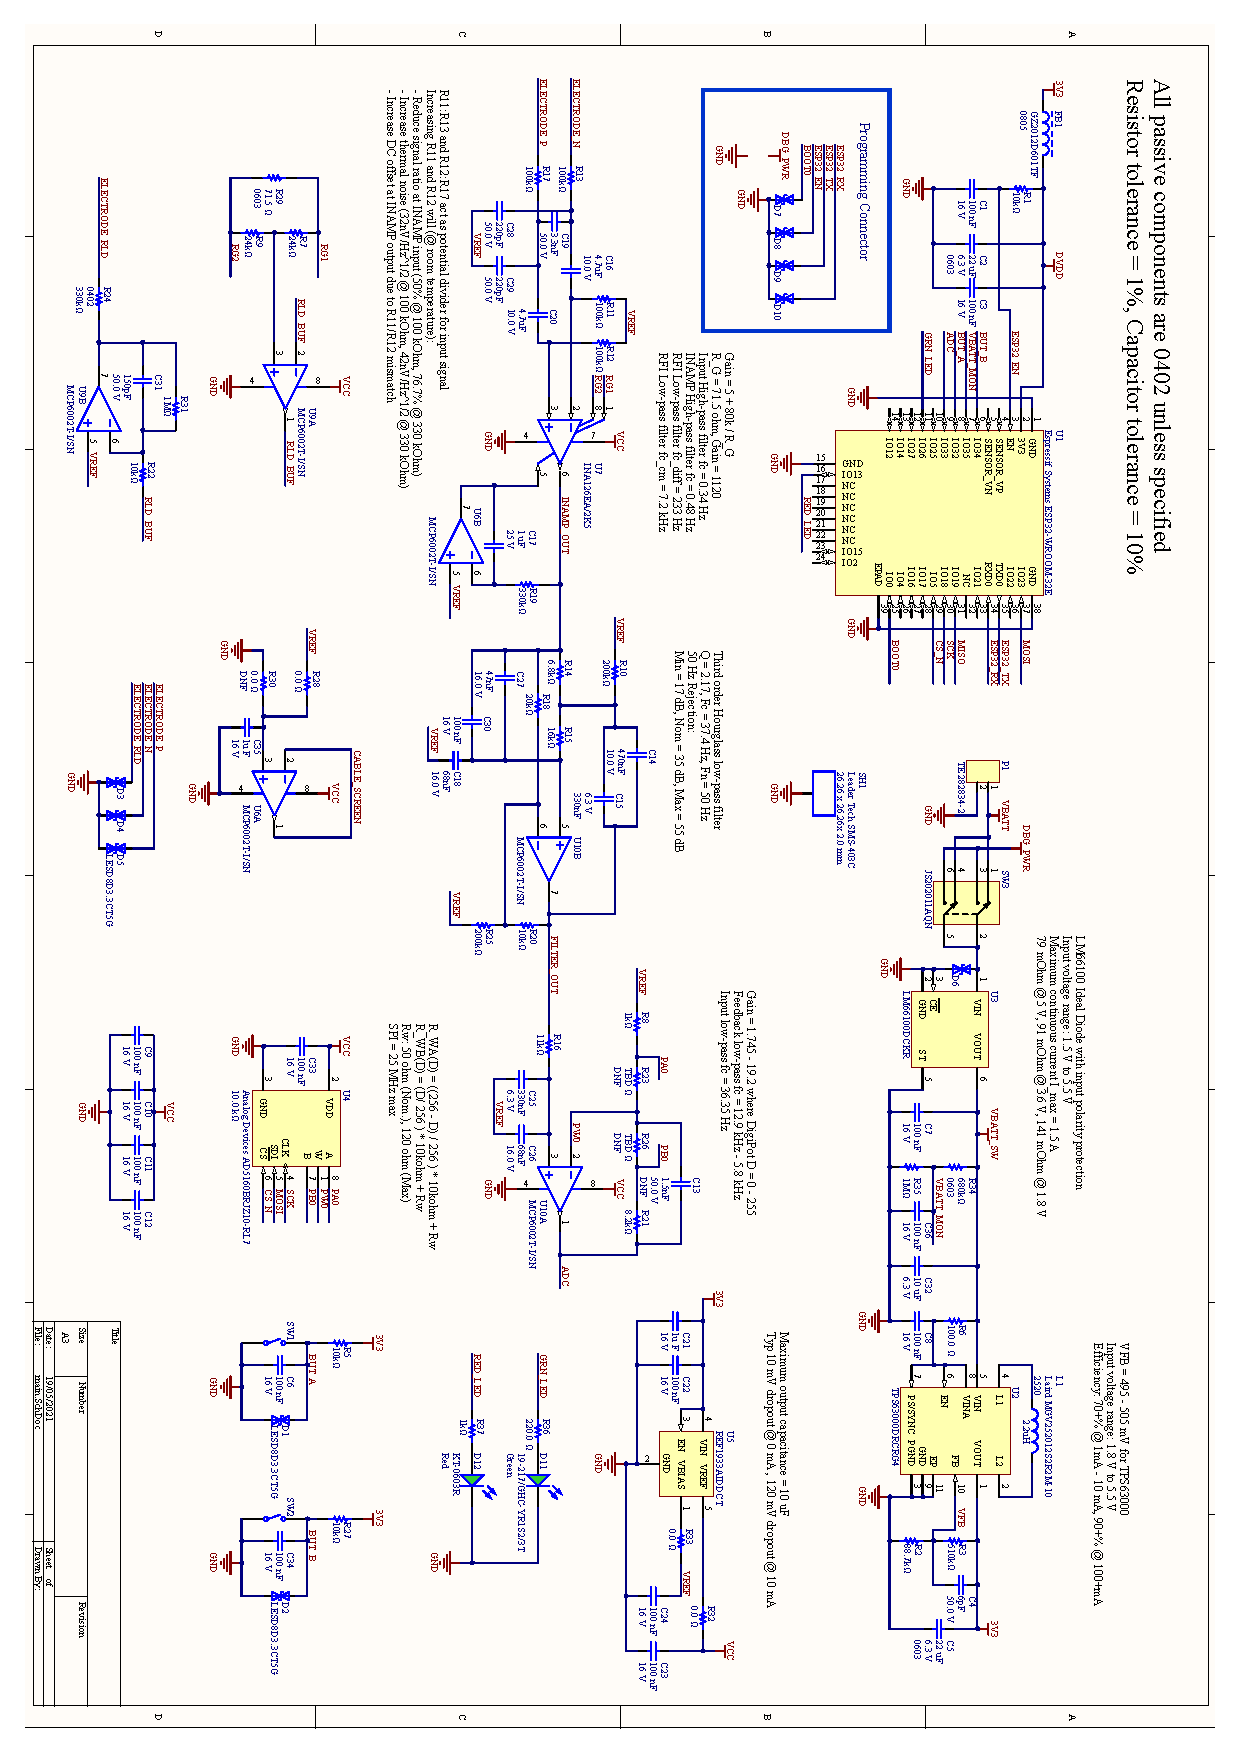
\includepdf[pages=-]{schematic.PDF}
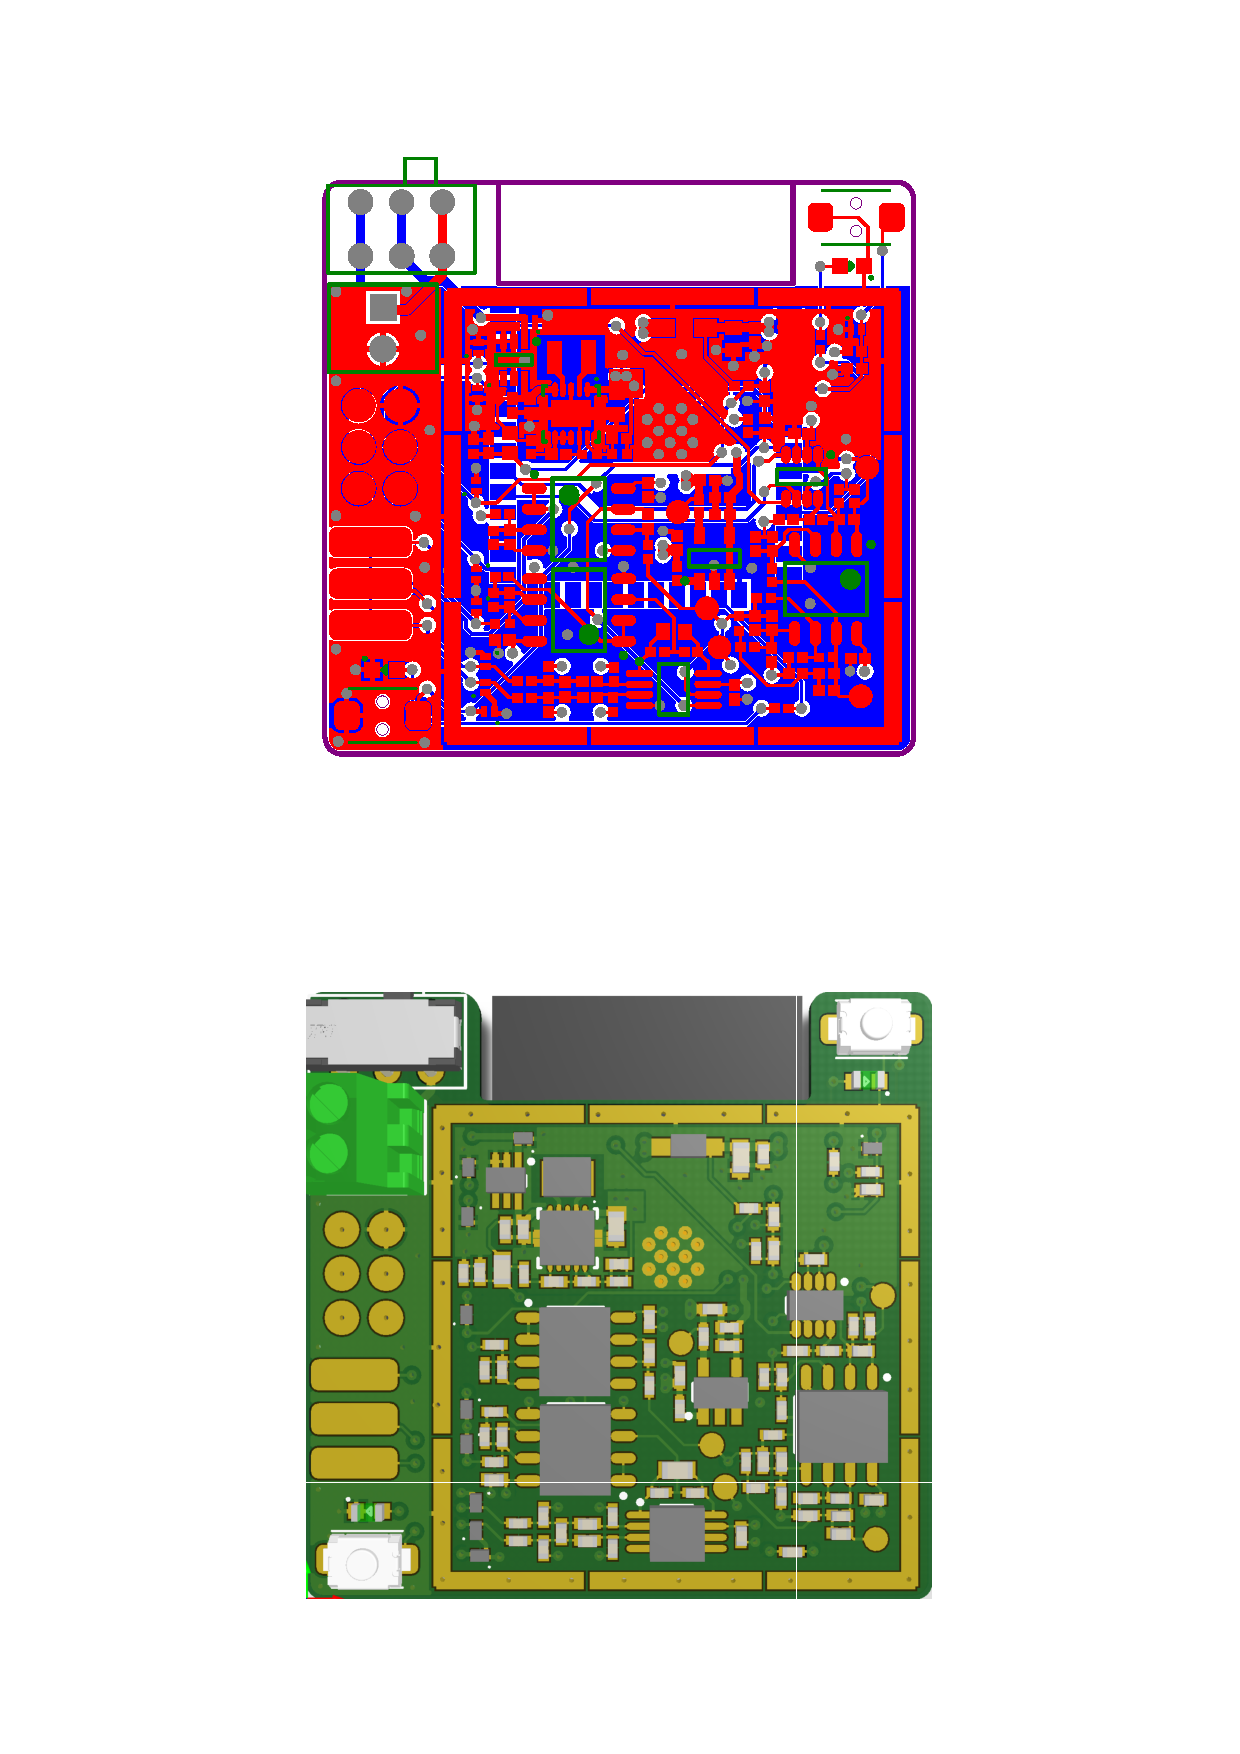
\includepdf[pages=-]{board-layouts.PDF}

\backmatter
\printbibliography

\end{document}
